\documentclass{article}

\usepackage{cancel}
\usepackage{tikz}
\usepackage{amsmath}
\usepackage{geometry}
\usepackage{graphicx}
\usepackage{amsfonts} 
\usepackage{verbatim}
\usepackage{mathrsfs}  
\usepackage{lmodern}
\usepackage{braket}
\usepackage{circuitikz}
\usepackage{steinmetz}
%\usepackage{movie15}


\usetikzlibrary{quotes,angles,decorations.pathmorphing,shapes.geometric,patterns}
\tikzset{snake it/.style={decorate, decoration=snake},
         block/.style = {draw, fill=white, very thick, rectangle, minimum height=1cm, minimum width=2cm},
         sum/.style= {draw, fill=white, very thick, circle, node distance=1cm},
         triangle/.style= {draw, fill=white, very thick, isosceles triangle, minimum height=2cm, minimum width=1cm},
         lblock/.style={draw,fill=white,very thick, rectangle, minimum height=3cm, minimum width=1cm},
         nblock/.style = {draw, very thick, rectangle, minimum height=1cm, minimum width=2cm}}
\numberwithin{equation}{subsection}
\graphicspath{ {./Immagini/} }

\renewcommand{\contentsname}{Indice}

%   To Do List:
%
%
% V Introduzione;
% V Modellistica;
% V Ingressi di Tipo Sinusoidale;
%   Controllori Digitali;
% V Esonero, potenzialmente;
%   Finire Con Equazioni Differenziali e Laplace;
% V Sostituire Immagini Screenate da Simulink con Blocchi Fatti in Tikz(https://latexdraw.com/block-diagram-in-latex-step-by-step-tikz-tutorial)e
%                                                                       (https://tex.stackexchange.com/questions/175969/block-diagrams-using-tikz);
%   Rotore DC grafico in CiruiTikz;
% X Figures Description;
%   Linearization;
%   Rumori Aleatori;
% V Figura Operazionale in Frequenza;
%   Reti Correttrici Grafico Circuito;
% V Schema \muC;
% V Grafico Quantizzazione;
% V Grafico Temporale Tc elaborazione controllore;
% V Grafico Impulso Discreto x(t);
% V Grafico Piano di Gauss x_c(s);
% V Grafico Shannon \omega_c;
% V Grafico Filtro Passa-Basso s->t;
%   Vera Forma Bode Segnale Campionato (trapezoide);
%   Parentesi Quadre funzioni Tempo Discreto;
%   \ref{eq://} anche su fisica;

\title{Fondamenti di Automatica}
\author{}
\date{}

\begin{document}

\maketitle

\clearpage

\tableofcontents

\clearpage

\section{Introduzione}

L'atumotica è la scienza che si occupa dell'analisi del controllo di sistemi dinamici in quattro passaggi:
\begin{itemize}
    \item Modellazione: Rappresentazione matematica basata sulla fisica del sistema;
    \item Studio delle Soluzioni: Le solusioni possono essere ottenute analiticamente, in forma chiusa, o tramite simulazioni del dato sistema;
    \item Esplorazione: Ricerca di relazioni tra struttura e comportamento del sistema ed approfondimento di quest'ultimo;
    \item Modifica e Controllo: RIcerca dei metodi per cambiare il comportamento del sistema.
\end{itemize}
Un sistema (dal greco s\'{y}n + hist\'{a}nai) viene definito come un insieme di oggetti connessi, indipendenti, che operano insieme.
La decomposizione funzionale di un sistema, è un tipo di scomposizione che esprime le relazioni causa-effetto necessarie per comprendere il 
funzionamento del sistema e per poter intervenire su di esso. 
Questa scomposizione è formata da vari blocchi funzionali, vengono rappresentati come degli oggetti aventi due ingressi e due uscite, e dei parametri 
interni che ne descrivono il legame, un singolo blocco funzionale può quindi essere analizzato come un sistema a sé. In un blocco funzionale possono 
entrare degli ingressi scelti arbitrariamente $u(t)$, di cui è possibile 
controllare li comportamento, e disturbi $z(t)$, ovvero errori che agiscono indipendentemente sul blocco, non controllabili. Da un blocco funzionale 
escono l'uscita $y(t)$, funzione rispetto alle entrate scelte, ed una catena di misura, usata per anlizzare uno o tutti i parametri di $y(t)$. 
Il comportamento di un singolo blocco viene rappresentato come dei parametri $\sum$ costanti, che rappresentano il comportamento fisico del blocco, 
e ne descrivono le sue uscite rispetto all'entrate date. 

\begin{center}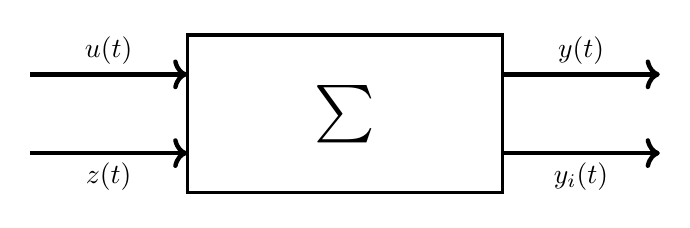
\begin{tikzpicture}[scale=2]

    \node[rectangle, draw, very thick, 
    minimum width = 4cm, 
    minimum height = 2cm] (r) at (0,0){\huge $\sum$};

    \draw[->,ultra thick](-2,0.25)--(-1,0.25);
    \node[above]at(-1.5,0.25){$u(t)$};

    \draw[->,ultra thick](-2,-0.25)--(-1,-0.25);
    \node[below]at(-1.5,-0.25){$z(t)$};

    \draw[->,ultra thick](1,0.25)--(2,0.25);
    \node[above]at(1.5,0.25){$y(t)$};

    \draw[->,ultra thick](1,-0.25)--(2,-0.25);
    \node[below]at(1.5,-0.25){$y_i(t)$};

\end{tikzpicture}\end{center}

Viene definito sistema isolato, un sistema in cui le uscite dipendono solo dagli ingressi attuali $\sum:y=f(u)$.

\begin{center}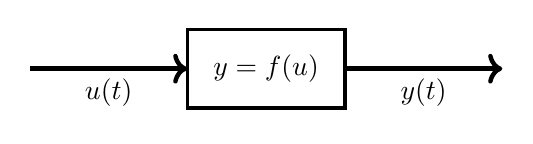
\begin{tikzpicture}[scale=2]
    \node[rectangle, draw, very thick, minimum width=2cm, minimum height=1cm](r)at(0,0){$y=f(u)$};

    \draw[->,ultra thick](-1.5,0)--(-0.5,0);
    \node[below]at(-1,0){$u(t)$};

    \draw[<-,ultra thick](1.5,0)--(0.5,0);
    \node[below]at(1,0){$y(t)$};

\end{tikzpicture}\end{center}

Viene definito sistema dinamico, un sistema le cui uscite dipendono dagli ingressi attuali e dagli ingressi passati del sistema 
$\sum:g(y^{(0)},...,y^{(n)},u^{(0)},...,u^{(m)})=0$.

\begin{center}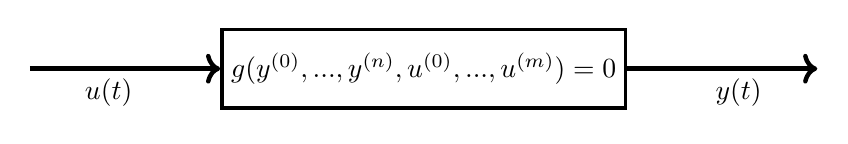
\begin{tikzpicture}[scale=2]
    \node[rectangle, draw, very thick, minimum width=2cm, minimum height=1cm](r)at(0,0){$g(y^{(0)},...,y^{(n)},u^{(0)},...,u^{(m)})=0$};

    \draw[->,ultra thick](-2.5,0)--(r.west);
    \node[below]at(-2,0){$u(t)$};

    \draw[<-,ultra thick](2.5,0)--(r.east);
    \node[below]at(2,0){$y(t)$};

\end{tikzpicture}\end{center}

Viene definito stato del sistema $\vec{x}(t)$, un vettore di $n$ variabili dipendenti dal tempo, tale che la conoscenza del suo valore 
allo stato $\vec{x}(t=0)$, e l'andamento dell'ingresso da $t=0$ in poi è sufficiente a determinare univocamente da $t=0$ in poi l'andamento di tutte le 
variabili dipendenti. 
In generale dato lo stato completo di un sistma in un istante di tempo $\vec{x}(t_0)$, è possible determinarne l'evoluzione futura, ovvero 
$\vec{x}(t>t_0)$. 

\clearpage

\section{Equazioni Differenziali}

\subsection{Introduzione alle Equazioni Differenziali}

\subsection{Equazioni Differenziali Ordinarie}

\subsection{Problema di Cauchy}

\subsection{Equazione Lineare di Primo Ordine}

\subsection{Equazione di Grado Superiore al Primo}

\subsubsection{Metodo Geometrico}

\subsubsection{Metodo Algebrico}

\clearpage

\section{Trasformata di Laplace}

\subsection{Trasformate Notevoli}

\subsection{Trasformata di un'Equazione Differenziale di Ordine Superiore al Primo}

\subsection{Stabilità di un Sistema}

\subsection{Funzioni di Trasferimento}
Una funzione di trasferimento del tipo ingresso-uscita, per cui perde ogni informazione sullo stato del sistema.
Se due funzioni di trasferimento si trovano in serie, allora si possono sostituire da un'altra funzione di trasferimento data dal prodotto dalle due, 
in generale per un numero $n$ di funzioni di trasferimento in serie si può descrivere una funzione equivalente $G(s)=\prod_{i=1}^nG_i(s)$. 

\begin{center}
    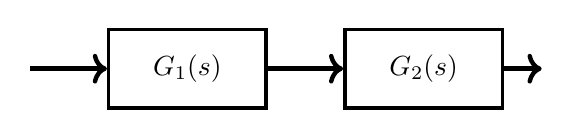
\begin{tikzpicture}[scale=2]
        \node[block, node distance=0cm](g1){$G_1(s)$};
        \node[block, right of=g1, node distance=3cm](g2){$G_2(s)$};
        \draw[->,ultra thick](g1.0)--(g2.180);
        \draw[->,ultra thick](-1,0)--(g1.180);
        \draw[->,ultra thick](g2.0)--(2.25,0);
    \end{tikzpicture}
\end{center}
\vspace{0.25cm}
\begin{center}
    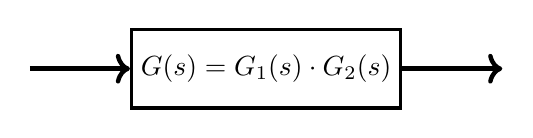
\begin{tikzpicture}[scale=2]
        \node[block, node distance=0cm](g){$G(s)=G_1(s)\cdot G_2(s)$};
        \draw[->,ultra thick](-1.5,0)--(g.180);
        \draw[->,ultra thick](g.0)--(1.5,0);
    \end{tikzpicture}
\end{center}

Date due funzioni di trasferimento in parallelo, potranno essere sostituite da un'altra funzinoe equivalente alla somma tra le due, in generale 
per $k$ funzioni di trasferimento in parallelo, potranno essere sostituite da un'altra funzione equivalente $G(s)=\sum_{i=1}^kG_i(s)$. 

\begin{center}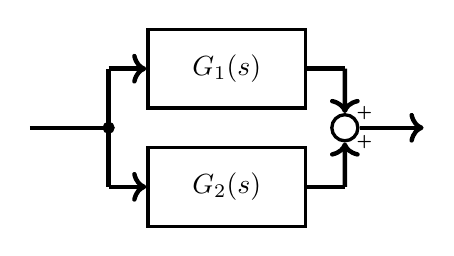
\begin{tikzpicture}[scale=2]
    \node[block, node distance=0cm](g1){$G_1(s)$};
    \node[block, below of=g1, node distance=1.5cm](g2){$G_2(s)$};
    \filldraw[black](-0.75,-0.375)circle(1pt)coordinate(split);
    \node[sum, right of=split, node distance=3cm](sum){};
    \draw[-,ultra thick](-1.25,-0.375)--(-0.75,-0.375);
    \draw[-,ultra thick](split)--(-0.75,0);
    \draw[-,ultra thick](split)--(-0.75,-0.75);
    \draw[->,ultra thick](-0.75,0)--(g1.180);
    \draw[->,ultra thick](-0.75,-0.75)--(g2.180);
    \draw[-,ultra thick](g1.0)--(0.75,0);
    \draw[-,ultra thick](g2.0)--(0.75,-0.75);
    \draw[->,ultra thick](0.75,0)--(sum.90)node[right]{$\scriptscriptstyle\boldsymbol{+}$};
    \draw[->,ultra thick](0.75,-0.75)--(sum.270)node[right]{$\scriptscriptstyle\boldsymbol{+}$};
    \draw[->,ultra thick](sum.0)--(1.25,-0.375);
\end{tikzpicture}\end{center}
\vspace{0.25cm}
\begin{center}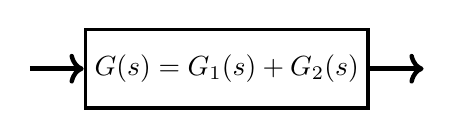
\begin{tikzpicture}[scale=2]
    \node[block](g){$G(s)=G_1(s)+G_2(s)$};
    \draw[->,ultra thick](-1.25,0)--(g.180);
    \draw[<-,ultra thick](1.25,0)--(g.0);
\end{tikzpicture}\end{center}

La funzione di trasferimento complessiva di un sistema presenta tutte le dinamiche di quel sistema, ovvero non viene persa l'informazione sulle 
dinamiche manipolando le funzioni di trasferimento. 
Per spostare una funzione di trasferimendo sulla catena bisogna opportunamente dividere e moltiplicare per tale funzione su tutte le altre 
ramificazioni per mantenere invariata l'entrata $U(s)$ su quella catena. 

\begin{center}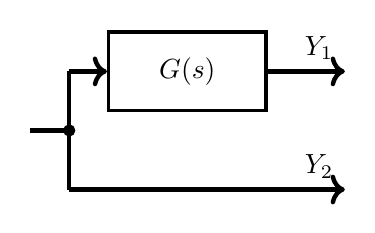
\begin{tikzpicture}[scale=2]
    \node[block](g){$G(s)$};
    \draw[-,ultra thick](-1,-0.375)--(-0.75,-0.375);
    \filldraw[black](-0.75,-0.375)circle(1pt);
    \draw[-,ultra thick](-0.75,-0.375)--(-0.75,0);
    \draw[->,ultra thick](-0.75,0)--(g.180);
    \draw[->,ultra thick](g.0)--(1,0)node[above left]{$Y_1$};
    \draw[-,ultra thick](-0.75,-0.375)--(-0.75,-0.75);
    \draw[->,ultra thick](-0.75,-0.75)--(1,-0.75)node[above left]{$Y_2$};
\end{tikzpicture}\end{center}
\vspace{0.25cm}
\begin{center}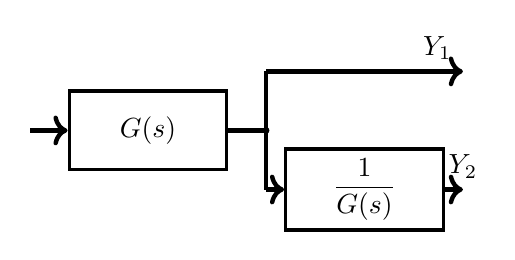
\begin{tikzpicture}
    \node[block](g){$\displaystyle\frac{1}{G(s)}$};
    \draw[-,ultra thick](-1.5,0.75)--(-1.25,0.75);
    \filldraw[black](-1.25,0.75)circle(1pt);
    \coordinate(o)at(-1.25,0.75);
    \draw[-,ultra thick](-1.25,0.75)--(-1.25,0);
    \draw[->,ultra thick](-1.25,0)--(g.180);
    \draw[->,ultra thick](g.0)--(1.25,0)node[above]{$Y_2$};
    \draw[-,ultra thick](-1.25,0.75)--(-1.25,1.5);
    \draw[->,ultra thick](-1.25,1.5)--(1.25,1.5)node[above left]{$Y_1$}; 
    \node[block, left of=o,node distance=1.5cm](g2){$G(s)$};
    \draw[-,ultra thick](g2.0)--(o);
    \draw[<-,ultra thick](g2.180)--(-4.25,0.75);
\end{tikzpicture}\end{center}

Viene definito processo di un sistema l'insieme coordinato di trasformazioni, trasmissione di energia, materiali e informazioni finalizzato ad un 
obiettivo, viene indicato con la funzione $P(s)$. 

Viene definito sistema a controreazione o retroreazione o feedback un sistema in cui l'uscita passata agisce sull'entrata futura. Si vuole calcolare 
una funzione di trasferimento equivalente:
\begin{equation}
    Y(s)=U(s)\cdot W(s)\Rightarrow W(s)=\displaystyle\frac{Y(s)}{U(s)}
\end{equation}    
Per trovarla si analizzano le varie entrate ed uscite del sistema. Quando si analizza una certa 
entrate o uscita, tutte le altre vengono consdierate nulle:
\begin{gather}
    \begin{cases}
        Y=eG\\
        e=U-HY
    \end{cases}\\
    \displaystyle\frac{Y}{G}=U-HY\\
    Y(1+GH)=UG\\
    \displaystyle\frac{Y}{U}=\frac{G}{1+GH}=W
\end{gather}
Viene definita la funzione del ciclo aperto, uguale al prodotto di ugni funzione di trasferimento lungo l'anello:
\begin{equation}
    F(s)=\prod_{i=1}^nG_i(s)
\end{equation}
Per cui la funzione di trasferimento del sistema a controreazione o funzione a ciclo chiuso può essere esrpessa come il rapporto tra la funzione di 
trasferimento a catena diretta, 
ovvere la funzione di trasferimento equivalente a tutte le funzioni di trasferimento tra l'ingresso $U$ all'uscita $Y$ senza passare per l'anello, e la 
somma tra $1$ e la funzione a ciclo aperto, con segno negativo se è presente un numero pari di cambi di segno, altrimenti positivo. 
\begin{equation}
    W(s)=\displaystyle\frac{G(s)}{1\pm F(s)}
\end{equation}

\begin{center}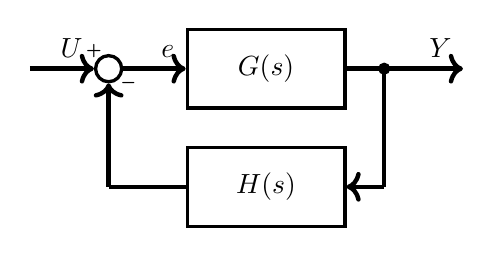
\begin{tikzpicture}[scale=2]
    \node[sum](sum)at(-1,0){};
    \draw[->,ultra thick](-1.5,0)--(sum.180)node[above left]{$U$}node[above]{$\scriptscriptstyle\boldsymbol{+}$};
    \node[block, right of=sum, node distance=2cm](g){$G(s)$};
    \draw[->,ultra thick](sum.0)--(g.180)node[above left]{$e$};
    \draw[-,ultra thick](g.0)--(0.75,0);
    \filldraw[black](0.75,0)circle(1pt);
    \draw[->,ultra thick](0.75,0)--(1.25,0)node[above left]{$Y$};
    \draw[-,ultra thick](0.75,-0.75)--(0.75,0);
    \node[block, below of=g, node distance=1.5cm](h){$H(s)$};
    \draw[->,ultra thick](0.75,-0.75)--(h.0);
    \draw[-,ultra thick](h.180)--(-1,-0.75);
    \draw[->,ultra thick](-1,-0.75)--(sum.270)node[right]{$\scriptscriptstyle\boldsymbol{-}$};
\end{tikzpicture}\end{center}

Se invece fosse presente un errore sulla catena diretta, allora per trovare la funzione a ciclo chiuso del disturbo, si considera:

\begin{gather}
    \begin{cases}
        e=-HY\\
        Y=eG+z
    \end{cases}\\
    Y=-GHY+z\\
    W_z=\displaystyle\frac{1}{1+GH}=\frac{1}{1+F}
\end{gather}

\begin{center}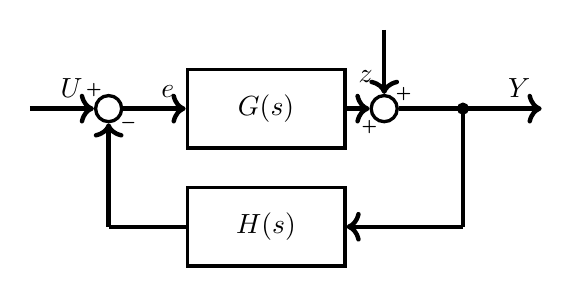
\begin{tikzpicture}[scale=2]
    \node[sum](sum)at(-1,0){};
    \node[sum](sum2)at(0.75,0){};
    \draw[->,ultra thick](-1.5,0)--(sum.180)node[above left]{$U$}node[above]{$\scriptscriptstyle\boldsymbol{+}$};
    \node[block, right of=sum, node distance=2cm](g){$G(s)$};
    \draw[->,ultra thick](sum.0)--(g.180)node[above left]{$e$};
    \draw[->,ultra thick](g.0)--(sum2.180)node[below]{$\scriptscriptstyle\boldsymbol{+}$};
    \draw[-,ultra thick](sum2.0)--(1.25,0);
    \filldraw[black](1.25,0)circle(1pt);
    \draw[->,ultra thick](0.75,0.5)--(sum2.90)node[above left]{$z$}node[right]{$\scriptscriptstyle\boldsymbol{+}$};
    \draw[->,ultra thick](1.25,0)--(1.75,0)node[above left]{$Y$};
    \draw[-,ultra thick](1.25,-0.75)--(1.25,0);
    \node[block, below of=g, node distance=1.5cm](h){$H(s)$};
    \draw[->,ultra thick](1.25,-0.75)--(h.0);
    \draw[-,ultra thick](h.180)--(-1,-0.75);
    \draw[->,ultra thick](-1,-0.75)--(sum.270)node[right]{$\scriptscriptstyle\boldsymbol{-}$};
\end{tikzpicture}\end{center}

Ogni errore sulla catena di misura genererà un'errore in uscita.\\

In generale la funzione a ciclo chiuso di una qualsiasi entrata di un qualsiasi sistema a controreazione avrà un denominatore $Dem(s)=1\pm F(s)$, dove $F(s)$ è la funzione a 
ciclo aperto del sistema considerato. Avendo tutte le stesso denominatore, 
se una funzione a ciclo chiuso per due generiche entrate e uscite del sistema è stabile, allora tutte le funzioni a ciclo chiuso del sistema sono 
stabili, e tutti gli oggetti in entrata saranno stabili.  

\clearpage

\section{Modellistica}

Per controllare il comportamento di un sistema, dopo aver analizzato l'entrata necessaria per ottenere l'effetto desiderato, si può 
implementare un controllore $C(s)$, che dato un ingresso lo manipola per poi restituirlo al processo $P(s)$ che agirà in base all'entrata modificata. 


Si può ottenere tramite un ciclo a feeedback:

\begin{center}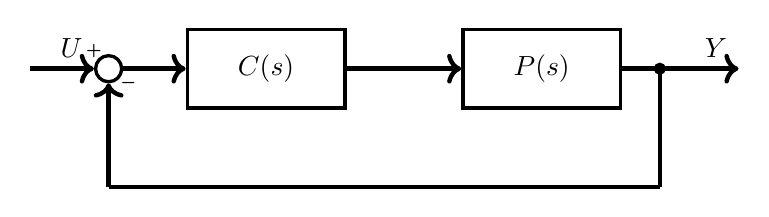
\begin{tikzpicture}[scale=2]
    \node[sum](sum)at(-1,0){};
    \draw[->,ultra thick](-1.5,0)--(sum.180)node[above left]{$U$}node[above]{$\scriptscriptstyle\boldsymbol{+}$};
    \node[block, right of=sum, node distance=2cm](c){$C(s)$};

    \draw[->,ultra thick](sum.0)--(c.180);
    \filldraw[black](2.5,0)circle(1pt);

    \draw[->,ultra thick](2.5,0)--(3,0)node[above left]{$Y$};
    \draw[-,ultra thick](2.5,-0.75)--(2.5,0);

    %\node[block]at(0.75,-0.75)(h){$H(s)$};
    \node[block]at(1.75,0)(p){$P(s)$};

    \draw[-,ultra thick](p.0)--(2.5,0);
    \draw[->,ultra thick](c.0)--(p.180);

    %\draw[->,ultra thick](2.5,-0.75)--(h.0);
    %\draw[-,ultra thick](h.180)--(-1,-0.75);
    \draw[-,ultra thick](2.5,-0.75)--(-1,-0.75);
    \draw[->,ultra thick](-1,-0.75)--(sum.270)node[right]{$\scriptscriptstyle\boldsymbol{-}$};
\end{tikzpicture}\end{center}

Oppure tramite un ciclo a feedforward, che userà un'altra funzione per manipolare l'ingresso non dipendente dalle uscite passate:


\begin{center}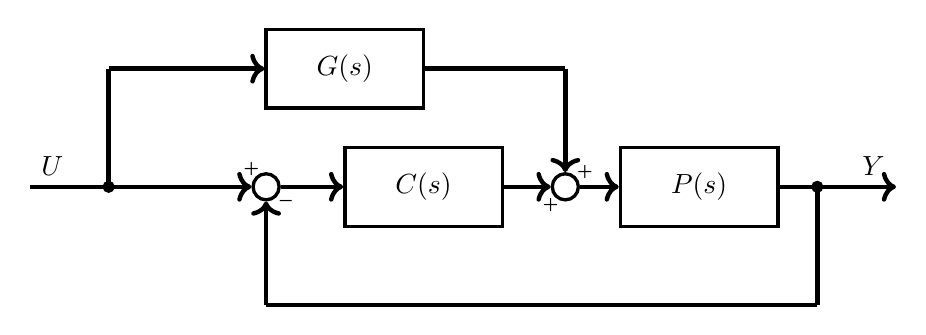
\begin{tikzpicture}[scale=2]
    \node[sum](sum)at(-1,0){};
    \draw[->,ultra thick](-1.5,0)--(sum.180)node[above]{$\scriptscriptstyle\boldsymbol{+}$};
    \filldraw[black](-2,0)circle(1pt);
    \draw[-,ultra thick](-2.5,0)node[above right]{$U$}--(-1.5,0);
    \node[block, right of=sum, node distance=2cm](c){$C(s)$};
    \node[sum]at(0.9,0)(sum2){};

    
    \draw[-,ultra thick](-2,0)--(-2,0.75);
    \node[block]at(-0.5,0.75)(g){$G(s)$};
    \draw[->,ultra thick](-2,0.75)--(g.180);
    \draw[-,ultra thick](g.0)--(0.9,0.75);
    \draw[->,ultra thick](0.9,0.75)--(sum2.90)node[right]{$\scriptscriptstyle\boldsymbol{+}$};



    \draw[->,ultra thick](sum.0)--(c.180);
    \filldraw[black](2.5,0)circle(1pt);

    \draw[->,ultra thick](2.5,0)--(3,0)node[above left]{$Y$};
    \draw[-,ultra thick](2.5,-0.75)--(2.5,0);

    %\node[block]at(0.75,-0.75)(h){$H(s)$};
    \node[block]at(1.75,0)(p){$P(s)$};

    \draw[-,ultra thick](p.0)--(2.5,0);
    \draw[->,ultra thick](c.0)--(sum2.180)node[below]{$\scriptscriptstyle\boldsymbol{+}$};
    \draw[->,ultra thick](sum2.0)--(p.180);

    %\draw[->,ultra thick](2.5,-0.75)--(h.0);
    %\draw[-,ultra thick](h.180)--(-1,-0.75);
    \draw[-,ultra thick](2.5,-0.75)--(-1,-0.75);
    \draw[->,ultra thick](-1,-0.75)--(sum.270)node[right]{$\scriptscriptstyle\boldsymbol{-}$};
\end{tikzpicture}\end{center}

\subsection{Motore a Corrente Continua}
Si vuole creare un modello per un motere elettrico, quindi si analizza il suo funzionamento. \\
Se una corrente attraversa una spira, crearà un campo magnetico, se sono 
presenti dei magneti permanenti ai lati della spira, verrà generata una forza magnetica che spinge sulla spira. Se la spira è in grado di ruotare su sé stessa, allora genererà 
un momento torcente. Per ottenere una rotazione continua bisogna invertire la corrente passante per la spira ogni mezzo giro, usando una corrente continua per ottenere ciò 
vengono usati dei contatti struscianti. In questo modo è possibile generare 
da una corrente continua e dei magneti peramnenti un momento torcente continuo. Per aumentare l'efficienza si fa ruotare il magnete all'interno di un cilindro contenete varie 
spire. Ogni volta che il magnete interno ruota di un certo angolo, si cambierà la coppia di spire che crea il campo magnetico, nonostante questo crei delle oscillazioni per 
il cambiamento di spire, la sua efficienza è notevolemente superiore ad un motore che usa contatti struscianti. \\
Si può rappresentare il circuito del rotore semplificato, formato da un'unica spira. In questo circuito semplificato sarà presente un generatore di tensione $V_a$, 
un resistore $R_a$, un induttore $L_a$, rappresentazione della spira, ed una forza contro elettro-motrice $f.c.em$, che rappresenta il magnete che ruota. 

%Ciruito in here, prova a immaginartelo eheheh. 

Per la seconda legge di Kirchoff si ottiene la seguente equazione della tensione di armatura:
\begin{equation}
    V_a=R_ai_a+L_a\dot i_a+f.c.em 
\end{equation}
La forza contro elettro-motrice generata dal magnete in rotazione è data da:
\begin{equation}
    f.c.em=\Phi_eK_a\omega\:,\:\Phi_eK_a=cost.\Rightarrow K_m=\Phi_eK_a
\end{equation}
Si avrà quindi un'equazione differenziale per la corrente, e si potrà ottenere la sua funzione di trasferimento:
\begin{gather}
    V_a=R_ai_a+L_a\dot i_a+K_m\omega\\
    V_a(s)=R_aI_a(s)+sL_aI_a(s)+K_m\Omega(s)\\
    I_a(s)=\displaystyle\frac{V_a-K_m\Omega(s)}{sL_a+R_a}
\end{gather}
Avrà un tempo caratteristico $\tau=\displaystyle\frac{1}{\displaystyle\left|\frac{R_a}{L_a}\right|}=\left|\frac{L_a}{R_a}\right|$. Questa corrente genererà una coppia 
$\tau(s)_m=K_mI_a(s)$. 
Per ottenere la rotazione del rotore bisogna esprimerla rispetto al mommento torcente prodotto. Considerando $J$ il momento di inerzia del carico, e $D$ la costante 
di attrito viscoso del rotore, si avrà:
\begin{gather}
    \tau_m(t)=J\dot\omega(t)+D\omega(t)\\
    \tau_m(s)=sJ\Omega(s)+D\Omega(s)\\
    \Omega(s)=\displaystyle\frac{\tau_m(s)}{sJ+D}
\end{gather}
Si può allora esprimere come un ciclo a controreazione:

\begin{center}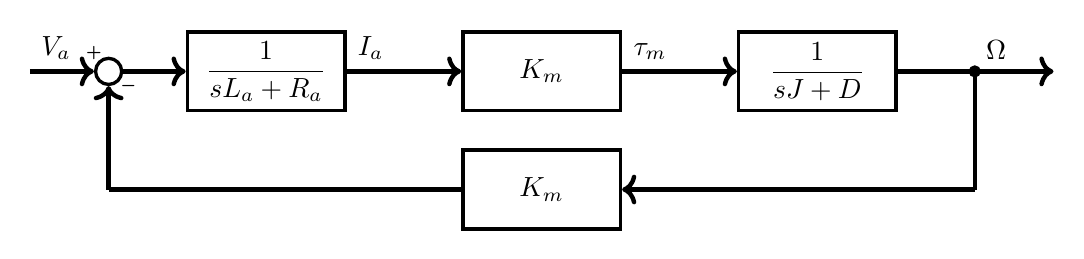
\begin{tikzpicture}[scale=2]
    \node[sum](sum)at(-1,0){};
    \draw[->,ultra thick](-1.5,0)node[above right]{$V_a$}--(sum.180)node[above]{$\scriptscriptstyle\boldsymbol{+}$};
    \node[block, right of=sum, node distance=2cm](c){$\displaystyle\frac{1}{sL_a+R_a}$};

    \draw[->,ultra thick](sum.0)--(c.180);
    \filldraw[black](4.5,0)circle(1pt);

    \draw[->,ultra thick](4.5,0)node[above right]{$\Omega$}--(5,0);
    \draw[-,ultra thick](4.5,-0.75)--(4.5,0);

    \node[block]at(1.75,-0.75)(h){$K_m$};
    \node[block]at(1.75,0)(p){$K_m$};
    \node[block]at(3.5,0)(j){$\displaystyle\frac{1}{sJ+D}$};

    \draw[->,ultra thick](p.0)node[above right]{$\tau_m$}--(j.180);
    \draw[-,ultra thick](j.0)--(4.5,0);
    \draw[->,ultra thick](c.0)node[above right]{$I_a$}--(p.180);

    \draw[->,ultra thick](4.5,-0.75)--(h.0);
    \draw[-,ultra thick](h.180)--(-1,-0.75);
    %\draw[-,ultra thick](2.5,-0.75)--(-1,-0.75);
    \draw[->,ultra thick](-1,-0.75)--(sum.270)node[right]{$\scriptscriptstyle\boldsymbol{-}$};
\end{tikzpicture}\end{center}
Per ottenere l'angolo al posto della velocità angolare del rotore, si può inserire un integratore $\displaystyle\frac{1}{s}$ sull'uscita $\Omega$. Per ottenere una velocità 
maggiore bisognerà allora aumentare il guadagno della funzione di trasferimento a ciclo chiuso $W(s)$. 

\subsection{Controllori}

Un controllore è un oggetto fisico usato per manipolare la stabilità di un sistema, il suo comportamento nel transitorio e a pieno regime. 
Esistono vari tipi di controllori, il più semplice è un controllore proporzionale che consiste di una costante $K_c$ che moltiplica l'ingresso, in modo 
che il processo lavori su un'entrata $Kc\cdot U$, se il controllore proporzionale vale $1$, avrà guadagno unitario. Per ottenere della catena 
diretta si moltiplica il guadagno del controllore, per il guadagno del processo: $K=K_c\cdot K_P$. Considerando un processo 
$P(s)=\displaystyle\frac{N(s)}{D(s)}$, si avrà una funzione a ciclo chiuso, per un controllore proporzionale: 

\begin{equation}
    W(s)=\displaystyle\frac{Kc\displaystyle\frac{N(s)}{D(s)}}{1+Kc\displaystyle\frac{N(s)}{D(s)}}=\frac{K_cN(s)}{D(s)+K_cN(s)}
\end{equation}

\begin{center}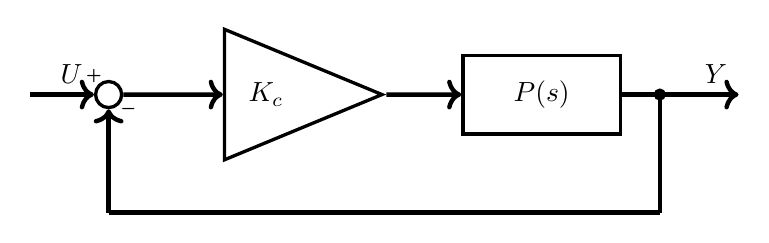
\begin{tikzpicture}[scale=2]
    \node[sum](sum)at(-1,0){};
    \draw[->,ultra thick](-1.5,0)--(sum.180)node[above left]{$U$}node[above]{$\scriptscriptstyle\boldsymbol{+}$};
    \node[triangle, right of=sum, node distance=2cm](c){$K_c$};

    \draw[->,ultra thick](sum.0)--(c.180);
    \filldraw[black](2.5,0)circle(1pt);

    \draw[->,ultra thick](2.5,0)--(3,0)node[above left]{$Y$};
    \draw[-,ultra thick](2.5,-0.75)--(2.5,0);

    %\node[block]at(0.75,-0.75)(h){$H(s)$};
    \node[block]at(1.75,0)(p){$P(s)$};

    \draw[-,ultra thick](p.0)--(2.5,0);
    \draw[->,ultra thick](c.0)--(p.180);

    %\draw[->,ultra thick](2.5,-0.75)--(h.0);
    %\draw[-,ultra thick](h.180)--(-1,-0.75);
    \draw[-,ultra thick](2.5,-0.75)--(-1,-0.75);
    \draw[->,ultra thick](-1,-0.75)--(sum.270)node[right]{$\scriptscriptstyle\boldsymbol{-}$};
\end{tikzpicture}\end{center}

\subsubsection{Luogo delle Radici}

Il teorema sulla continuità delle radici di un polinomio descrive il comportamento delle soluzioni di un polinomio, alterando leggermente i 
valori dei coefficienti del polinomio:
\begin{quotation}
    Considerando un polinomio $P^n(x)=a_nx^n+...a_1x=0$, sarà sempre possibile trovare una soluzione $x_0'$ nell'intorno $I_{\varepsilon}(x_0)$, dove $x_0$ 
    è una soluzione di $P(x)$, al polinomio $P'(x)=(a_n+\varepsilon)x^n+...(a_1+\varepsilon)x=0$, per ogni $\varepsilon>0$ scelto arbitrariammente. 
\end{quotation} 
Per cui se esiste almeno una soluzione di $D(s)+K_cN(s)$, allora sarà sempre possibile trovare una sua soluzione per ogni valore di $K_c$ scelto. 
Per valori di $K_c\approx0$, si potrà approssimare il denominatore a: $D(s)+K_cN(s)\approx D(s)$, quindi il valore dei poli sarà dato dalla sola 
funzione $D(s)$, al contrario per valori del guadagno del controllore molto elevati  $K_c>>0$, si avrà $D(s)+K_cN(s)\approx N(s)$, quindi il valore 
dei poli sarà dato dalla sola funzione $N(s)$. 
Per controllare l'andamento dei poli della funzione a ciclo chiuso rispetto ai valori del guadagno del controllore, si usa il luogo delle radici, un 
grafico che che mostra lo spostamento dei poli rispetto all'aumento del guadadno, i poli partiranno dai valori dei poli del processo, fino a tendere 
al valore degli zeri del processo. Se il processo presenta un numero minore di zeri, allora alcuni dei poli tenderanno all'infinito. 
Il luogo della radici viene rappresentato su un piano di Gauss. Se due poli sono complessi e coinugati, allora il loro comportamento rispetto all'
aumentare del guadagno sarà simmetrico. Questi poli possono essere espressi come: 
\begin{equation}
    (s+p_1)(s+p_1^*)=\displaystyle\frac{s^2}{\omega_0^2}+\frac{2\xi}{\omega_0}s+1
\end{equation}
Dove $\xi$ rappresenta lo smorzamento del polo, quantifica quanto persiste l'oscillazione del sistema in seguito ad un dato ingresso, è dato da 
$\xi=cos\varphi$, dove $\varphi$ rappresenta l'angolo con l'orizzontale rispetto a $\omega_0$, la distanza tra l'origne $O$ ed il polo, che esprime 
l'ampiezza dell'oscillazione. 
Per cui il polo espresso in coordinate polari sarà $(\omega_0,\:\varphi)$. 
Un polo con uno smorzamento maggiore tenderà a convergere più velocemente, e avrà un tempo caratteristico minore. \\
In matalab si può ottenere il grafico del luogo delle radici per qualsiasi funzione di trasferimento tramite il comando 
La funzione di trasferimento sarà stabile se il luogo delle radici è intermaente nel semipiano di parte reale negativa, altrimenti sarà stabile solo 
in un certo intervallo di $K_c$. La funzione "rlocus(F)" analizza solo valori positivi del guadagno, per controllare se l'intervallo si estenda anche per 
valori negativi bisogna controllare "rlocus(-F)". Le linee radiali uscenti dall'origine rappresentano le linee di smorzamento. 
I punti segnati con una croce rappresetano i poli, mentre i punti indiviuati da un cerchio rappresentano gli zeri della funzione.\\
Aumentando il guadagno, aumenta l'ampiezza di un'oscillazione e diminuisce l'errore che ne deriva. La robustezza di un sistema è una misura che 
quantifica quanto un sistema mantiene nel sue dinamiche nel tempo, rispetto ad errori. 

\begin{center}
    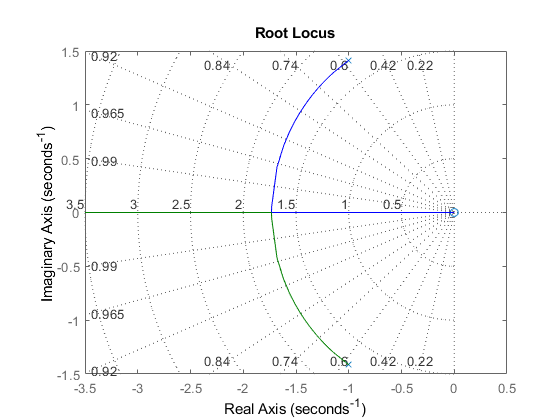
\includegraphics[scale=0.55]{rlocus}
    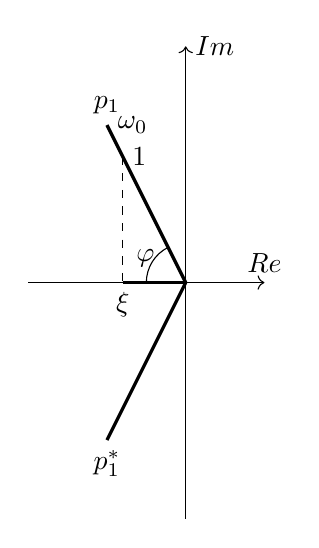
\begin{tikzpicture}[scale=2]
    \coordinate(O)at(0,0);
    \draw[->](-1,0)coordinate(Re)--(0.5,0)node[above]{$Re$};
    \draw[->](0,-1.5)--(0,1.5)coordinate(Im)node[right]{$Im$};

    \draw[-,very thick](O)--(-0.5,1)coordinate(w)node[right]{$\omega_0$}node[above]{$p_1$};
    \draw[-,very thick](O)--(-0.5,-1)node[below]{$p_1^*$};
    \draw[dashed](-0.4,0.8)node[right]{$1$}--(-0.4,0)node[below]{$\xi$};
    \draw[-,thick](-0.4,0)--(0,0);
    \pic["$\varphi$",draw, angle eccentricity=1.2, angle radius=0.5cm]{angle=w--O--Re};

    \end{tikzpicture}
\end{center}

\subsubsection{Controllore Proporzionale con un integratore}
Per controllare l'effetto di un controllore proporzionale sul guadadno di un sistema, si considera un'entrata a gradino $U(s)=\displaystyle\frac{1}{s}$, e si calcola con 
il teorma del valore finale il valore dell'uscita a regime permanente:
\begin{gather}
    W(s)=\displaystyle\frac{Y(s)}{U(s)}=\frac{K_cN(s)}{D(s)+K_cN(s)}\\
    Y(s)=\displaystyle\frac{K_c N(s)}{D(s)+K_c N(s)}\frac{1}{s}\\
    K_Y=\lim_{s\to0}s\cdot Y(s)=\lim_{s\to0}s\displaystyle\frac{K_c N(s)}{D(s)+K_c N(s)}\frac{1}{s}\\
    K_Y=\displaystyle\frac{K_c}{\displaystyle\frac{1}{K_P}+K_c}<1
\end{gather}
Dove $K_P$ è il guadagno del proceso $P(s)$. Per valori piccoli di $K_c$, si avrà un errore $e_Y=1-K_Y$ elevato, solo all'umentare di $K_c$ l'errore diminuirà fino a tendere 
a $1$ per $K_c\to\infty$: 
\begin{equation}
    e_Y=1-\lim_{K_c\to\infty}\displaystyle\frac{K_c}{\displaystyle\frac{1}{K_P}+K_c}=1-1=0
\end{equation}
Si vuole ottenere un'errore nullo senza aumentare il guadagno $K_c$, poiché cambierebbe l'andamento del processo nel transitorio. Inserendo un integratore insieme ad 
un controllore proporzionale $\displaystyle\frac{K_c}{s}$ si avrà una funzione a ciclo chiuso:
\begin{equation}
    W(s)=\displaystyle\frac{K_cN(s)}{sD(s)+K_cN(s)}
\end{equation}
Il guadagno dell'uscita per un'entrata a gradino sarà in questo caso:
\begin{equation}
    K_Y=\lim_{s\to0}s\displaystyle\frac{K_c N(s)}{sD(s)+K_c N(s)}\frac{1}{s}=\frac{K_c}{0\cdot\displaystyle\frac{1}{K_P}+K_c}=1
\end{equation}
Si può quindi ottenere un'errore nullo a regime permanente, indipendentemente dal valore del controllore prooprzionale. Da notare come per ottenere un errore nullo è stato 
necessario inserire un integratore, per un'entrata a gradino. Per il principio del modello interno per ottenere un'uscita di un certo tipo sarà necessaria una dinamica 
simile all'initerno del sistema. Segue che per un sistema asintoticamente stabile, l'uscita seguirà l'entrata, ovvero entrambe saranno dello stesso tipo. 

\begin{center}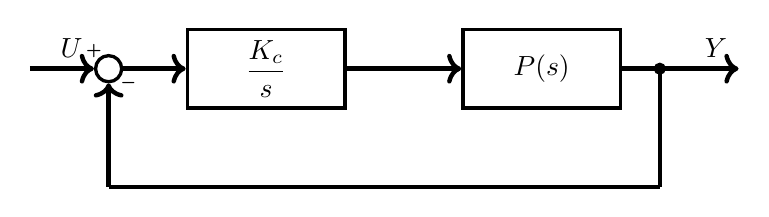
\begin{tikzpicture}[scale=2]
    \node[sum](sum)at(-1,0){};
    \draw[->,ultra thick](-1.5,0)--(sum.180)node[above left]{$U$}node[above]{$\scriptscriptstyle\boldsymbol{+}$};
    \node[block, right of=sum, node distance=2cm](c){$\displaystyle\frac{K_c}{s}$};

    \draw[->,ultra thick](sum.0)--(c.180);
    \filldraw[black](2.5,0)circle(1pt);

    \draw[->,ultra thick](2.5,0)--(3,0)node[above left]{$Y$};
    \draw[-,ultra thick](2.5,-0.75)--(2.5,0);

    %\node[block]at(0.75,-0.75)(h){$H(s)$};
    \node[block]at(1.75,0)(p){$P(s)$};

    \draw[-,ultra thick](p.0)--(2.5,0);
    \draw[->,ultra thick](c.0)--(p.180);

    %\draw[->,ultra thick](2.5,-0.75)--(h.0);
    %\draw[-,ultra thick](h.180)--(-1,-0.75);
    \draw[-,ultra thick](2.5,-0.75)--(-1,-0.75);
    \draw[->,ultra thick](-1,-0.75)--(sum.270)node[right]{$\scriptscriptstyle\boldsymbol{-}$};
\end{tikzpicture}\end{center}

\subsubsection{Entrata di Tipo $k$}

Poiché l'uscita tenderà a seguire l'entrata, si considera un modello di riferimento ideale, dove l'uscita $Y_d$ è proporzionale all'entrata di un fattore $K_d$:
\begin{equation}
    Y_d=K_d\cdot U\Rightarrow W_d(s)=K_d
\end{equation}
Ma non potrà esistere un sistema fisico tale da avere una funzione a ciclo chiuso uguale ad una costante. Per cui si vuole calcolare l'errore di un sistema rispetto a 
questo riferimento ideale, per ottenerlo si considera: 

\begin{center}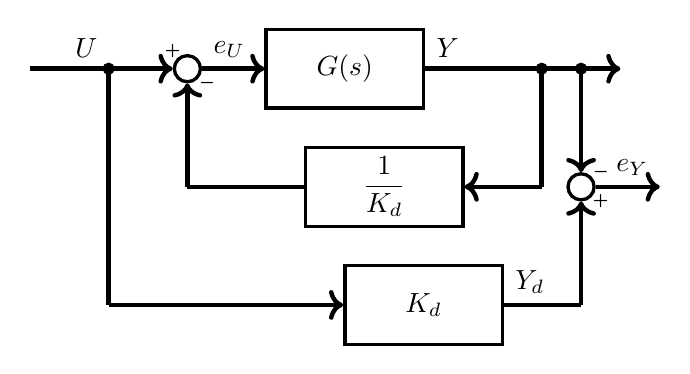
\begin{tikzpicture}[scale=2]
    \node[sum](sum)at(-1,0){};
    \draw[->,ultra thick](-1.5,0)--(sum.180)node[above]{$\scriptscriptstyle\boldsymbol{+}$};
    \draw[-,ultra thick](-2,0)--(-1.5,0)node[above left]{$U$};
    \filldraw[black](-1.5,0)circle(1pt);
    %\node[triangle, right of=sum, node distance=2cm](c){$K_c$};

    %\draw[->,ultra thick](sum.0)--(c.180);
    \filldraw[black](1.25,0)circle(1pt);
    \filldraw[black](1.5,0)circle(1pt);
    \draw[-,ultra thick](1.25,0)--(1.5,0);
    \draw[->,ultra thick](1.5,0)--(1.75,0);

    %\draw[->,ultra thick](2.5,0)--(3,0)node[above left]{$Y$};
    %\draw[-,ultra thick](2.5,-0.75)--(2.5,0);

    \node[block]at(0.25,-0.75)(h){$\displaystyle\frac{1}{K_d}$};
    \node[block, right of=sum, node distance=2cm](p){$G(s)$};
    \draw[->,ultra thick](sum.0)node[above right]{$e_U$}--(p.180);
    \draw[-,ultra thick](p.0)node[above right]{$Y$}--(1.25,0);
    %\draw[->,ultra thick](c.0)--(p.180);

    \draw[-,ultra thick](1.25,0)--(1.25,-0.75);
    \draw[->,ultra thick](1.25,-0.75)--(h.0);
    \draw[-,ultra thick](h.180)--(-1,-0.75);
    %\draw[-,ultra thick](2.5,-0.75)--(-1,-0.75);
    \draw[->,ultra thick](-1,-0.75)--(sum.270)node[right]{$\scriptscriptstyle\boldsymbol{-}$};

    \node[sum](sum2)at(1.5,-0.75){};
    \draw[->,ultra thick](1.5,0)--(sum2.90)node[right]{$\scriptscriptstyle\boldsymbol{-}$};
    \node[block](k)at(0.5,-1.5){$K_d$};
    \draw[-,ultra thick](k.0)node[above right]{$Y_d$}--(1.5,-1.5);
    \draw[->,ultra thick](1.5,-1.5)--(sum2.270)node[right]{$\scriptscriptstyle\boldsymbol{+}$};

    \draw[-,ultra thick](-1.5,0)--(-1.5,-1.5);
    \draw[->,ultra thick](-1.5,-1.5)--(k.180);

    \draw[->,ultra thick](sum2.0)--(2,-0.75)node[above left]{$e_Y$};

\end{tikzpicture}\end{center}

Si avrà quindi un errore in entrata $e_U$ dovuto alla differenza tra la funzione a ciclo chiuso ed il modello ideale: 
\begin{equation}
    e_U=U-\displaystyle\frac{Y}{K_d}
\end{equation}
questo errore sarà nullo per valori di uscita uguali al riferimento ideale: $Y=Y_d=K_dU$.\\
Si avrà un errore in uscita:
\begin{gather}
    e_Y:E(s)=Y_d-Y=K_dU(s)-W(s)U(s)\\
    K_dU(s)-\displaystyle\frac{K_dG(s)}{K_d+G(s)}U(s)\\
    \left(\displaystyle\frac{K_d^2+K_dG(s)-K_dG(s)}{K_d+G(s)}\right)U(s)\\
    E(s)=\displaystyle\frac{K_d^2}{K_d+G(s)}U(s)
\end{gather}
Per cui è necessario conoscere l'ingresso del sistema per poter determinare l'errore in uscita. Si analizza il caso di entrate del tipo $k$ polinomiale: 
\begin{equation}
    u(t)=\displaystyle\frac{t^k}{k!}=\delta_{-(k+1)}(t)\Rightarrow U(s)=\displaystyle\frac{1}{s^{k+1}}
\end{equation}
Si considera il processo $G(s)$ contente un numero $h$ di integratori:
\begin{equation}
    G(s)=\displaystyle\frac{G'(s)}{s^h}
\end{equation}

Allora si avrà un errore in uscita:
\begin{equation}
    E(s)=\displaystyle\frac{K_d^2}{K_d+\displaystyle\frac{G'(s)}{s^h}}\frac{1}{s^{(k+1)}}
\end{equation}
Si vuole determinare per quali valore di $h$ si ha un errore nullo a regime permanetne, per cui si analizza: 
\begin{equation}
    \lim_{s\to0}s\cdot E(s)=\lim_{s\to0}s\cdot\displaystyle\frac{K_d^2}{K_d+\displaystyle\frac{G'(s)}{s^h}}\frac{1}{s^{(k+1)}}=\frac{K_d^2}{G'(0)}\lim_{s\to0}\frac{1}{s^{k-h}}
\end{equation}
Si definisce guadagno generalizzato $K_G$ di una funzione $G(s)=\displaystyle\frac{G'(s)}{s^h}$, il suo valore per $s=0$, senza considerare gli integratori, per cui: $K_G=G'(0)$. 
Per cui l'errore in uscita e pieno regime dipenderà dal numero di integratori nel processo $G$:
\begin{equation}
    \displaystyle\frac{K_d^2}{K_G}\lim_{s\to0}\frac{1}{s^{k-h}}=
    \begin{cases}
        +\infty,\:k>h\\
        \displaystyle\frac{K_d^2}{K_G},\:k=h\\
        0,\:k<h
    \end{cases}
\end{equation}
Segue che per rigettare un errore di tipo $k$, serviranno $k$ integratori nella catena diretta. Anche se inserire un numero maggiore di integratori annulla l'errore, non è 
consigliato inserire un numero maggiore dell'indispensabile di integratori nella catena diretta, poiché più aumenta il numero di poli nell'origine più il sistema tende all'
instabilità. Viene definito sistema di controllo di tipo $k$, un controllore tale da rendere l'errore a regime permanente costante per un'entrta di tipo $k$. Da notare che 
per un entrata di tipo $0$, non serviranno integratori e l'errore a regime permanente sarà dato da: $E_Y=\displaystyle\frac{K_d^2}{K_d+K_G}$. \'{E} possibile quindi 
creare una tabella che mostri l'andamento dell'errore rispetto ad entrate di tipo $k$ e un numero $h$ di integratori in catena diretta:

\begin{center}
    \begin{tabular}{|c|c|c|c|c}
        \hline
        $h,\:k$ & $0$ & $1$ & $2$ & $\ldots$\\[0.5ex]
        \hline
        $0$ & $\displaystyle\frac{K_d^2}{K_d+K_G}$ & $\infty$ &$\infty$\\[0.5ex]
        \hline
        $1$ & $0$ & $\displaystyle\frac{K_d^2}{K_G}$ & $\infty$\\[0.5ex]
        \hline
        $2$ & $0$ & $0$ & $\displaystyle\frac{K_d^2}{K_G}$\\[0.5ex]
        \hline
        $\vdots$ & & & & $\ddots$\\
    \end{tabular}
\end{center}

\begin{center}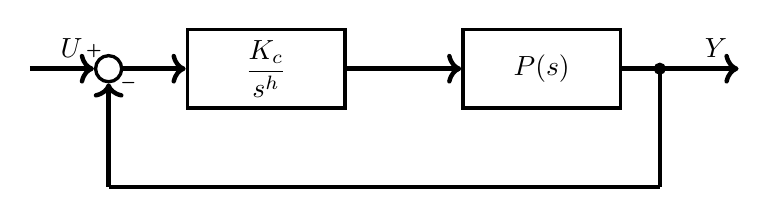
\begin{tikzpicture}[scale=2]
    \node[sum](sum)at(-1,0){};
    \draw[->,ultra thick](-1.5,0)--(sum.180)node[above left]{$U$}node[above]{$\scriptscriptstyle\boldsymbol{+}$};
    \node[block, right of=sum, node distance=2cm](c){$\displaystyle\frac{K_c}{s^h}$};

    \draw[->,ultra thick](sum.0)--(c.180);
    \filldraw[black](2.5,0)circle(1pt);

    \draw[->,ultra thick](2.5,0)--(3,0)node[above left]{$Y$};
    \draw[-,ultra thick](2.5,-0.75)--(2.5,0);

    %\node[block]at(0.75,-0.75)(h){$H(s)$};
    \node[block]at(1.75,0)(p){$P(s)$};

    \draw[-,ultra thick](p.0)--(2.5,0);
    \draw[->,ultra thick](c.0)--(p.180);

    %\draw[->,ultra thick](2.5,-0.75)--(h.0);
    %\draw[-,ultra thick](h.180)--(-1,-0.75);
    \draw[-,ultra thick](2.5,-0.75)--(-1,-0.75);
    \draw[->,ultra thick](-1,-0.75)--(sum.270)node[right]{$\scriptscriptstyle\boldsymbol{-}$};
\end{tikzpicture}\end{center}

\subsubsection{Disturbo di Tipo $k$}

Nel caso sia presente un disturbo di tipo $k$ sulla catena diretta $z(t)=\delta_{-(k+1)}(t)$, per rigettarlo a regime permanente bisogna ottenere un'errore nullo in uscita 
considerando il disturbo come unica entrata del sistema. 

\begin{center}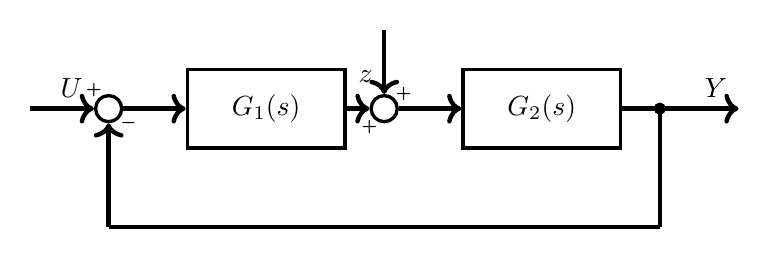
\begin{tikzpicture}[scale=2]
    \node[sum](sum)at(-1,0){};
    \node[sum](sum2)at(0.75,0){};
    \draw[->,ultra thick](-1.5,0)--(sum.180)node[above left]{$U$}node[above]{$\scriptscriptstyle\boldsymbol{+}$};


    \node[block, right of=sum, node distance=2cm](g){$G_1(s)$};
    \draw[->,ultra thick](sum.0)--(g.180);
    \draw[->,ultra thick](g.0)--(sum2.180)node[below]{$\scriptscriptstyle\boldsymbol{+}$};
    

    \filldraw[black](2.5,0)circle(1pt);


    \draw[->,ultra thick](0.75,0.5)--(sum2.90)node[above left]{$z$}node[right]{$\scriptscriptstyle\boldsymbol{+}$};

    \node[block]at(1.75,0)(k){$G_2(s)$};
    \draw[->,ultra thick](sum2.0)--(k.180);
    \draw[-,ultra thick](k.0)--(2.5,0);

    \draw[->,ultra thick](2.5,0)--(3,0)node[above left]{$Y$};
    \draw[-,ultra thick](2.5,-0.75)--(2.5,0);


    %\node[block, below of=g, node distance=1.5cm](h){$H(s)$};
    %\draw[->,ultra thick](1.25,-0.75)--(h.0);
    %\draw[-,ultra thick](h.180)--(-1,-0.75);
    \draw[-,ultra thick](2.5,-0.75)--(-1,-0.75);
    \draw[->,ultra thick](-1,-0.75)--(sum.270)node[right]{$\scriptscriptstyle\boldsymbol{-}$};
\end{tikzpicture}\end{center}

Allora si avrà una funzione a ciclo chiuso del disturbo:
\begin{equation}
    W_z(s)=\displaystyle\frac{G_2(s)}{1+G_1(s)G_2(s)}
\end{equation}
Ed un'uscita a regime permanente $Y_z$:
\begin{equation}
    Y_z=\lim_{s\to0}s\cdot\displaystyle\frac{G_2(s)}{1+G_1(s)G_2(s)}\frac{1}{s^{k+1}}
\end{equation}
Per poter rigettare il disturbo bisogna inserire $k$ integratori a monte di esso, ovvero nella funzione $G_1(s)$, l'errore causato a regime permanente allora sarà:
\begin{gather}
    Y_z=\lim_{s\to0}s\cdot\displaystyle\frac{G_2(s)}{1+\displaystyle\frac{G_1'(s)}{s^k}G_2(s)}\frac{1}{s^{k+1}}=\frac{K_{G_2}}{K_{G_1}K_{G_2}}
\end{gather}

Per cui per inseguire o rigettare un polinomio di tipo $k$ in entrata, servono $k$ integratori in catena diretta, a monte del disturbo. Gli integratori nella funzinoe $G_1$ 
annulano l'errore per un entrata di tipo $k$ e rigettano un disturbo di tipo $k$. Ma l'inserimento di poli nell'orgine 
destabilizza il sistema, quindi è necessario inserire un altro elemento per recuperare la stabilità. \\ 

Considerando il motore a corrente diretta, un possible disturbo potrebbe essere il peso del carico che sta spostando che produrra un momento torcente costante nel tempo, 
per cui sarà un disturbo di tipo $0$ e necessiterà di un controllore di tipo $0$ a monte del disturbo. Nel caso di un motore, si considera un riferimento ideale legato da 
una cosante unitaria: $Y_d=U$, ovvero per una qualsiasi entrata, l'uscita la deve seguire esattamente. Per cui l'errore risultarà: $e=\displaystyle\frac{1}{1+K_cK_{DC}}$, 
dove $K_c$ è il guadagno del controllore di tipo $0$. Se il motore opera dei sistemi precisi, richiederanno un'errore nullo 
indipendentemente dal valore del guadagno del controllore quindi si userà un controllore di tpo $1$, ma ciò renderà il transitorio molto lungo, poiché un integratore 
prima di diventare utile dovrà caricarsi per un certo intervallo di tempo, prima di agire come richiesto. Ciò altererà i punti di equilibrio del rotore, ma inserire un 
altro integratore per rigettare l'errore renderebbe il sistema instabile, per cui si può alterare manualmente il riferimento iniziale su cui opera il sistema. 

\begin{center}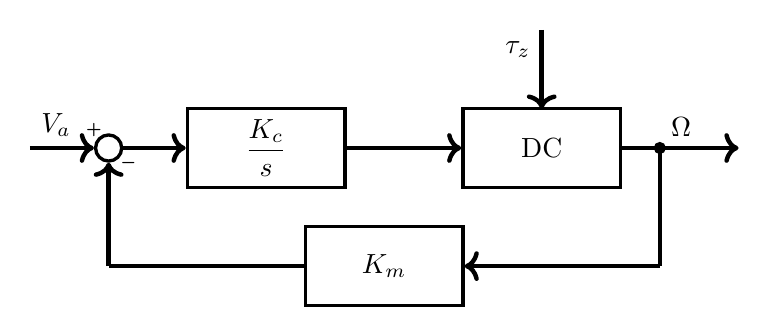
\begin{tikzpicture}[scale=2]
    \node[sum](sum)at(-1,0){};
    \draw[->,ultra thick](-1.5,0)node[above right]{$V_a$}--(sum.180)node[above]{$\scriptscriptstyle\boldsymbol{+}$};
    \node[block, right of=sum, node distance=2cm](c){$\displaystyle\frac{K_c}{s}$};

    \draw[->,ultra thick](sum.0)--(c.180);
    \filldraw[black](2.5,0)circle(1pt);

    \draw[->,ultra thick](2.5,0)node[above right]{$\Omega$}--(3,0);
    \draw[-,ultra thick](2.5,-0.75)--(2.5,0);

    \node[block]at(0.75,-0.75)(h){$K_m$};
    \draw[->,ultra thick](1.75,0.75)node[below left]{$\tau_z$}--(1.75,0.25);
    \node[block]at(1.75,0)(p){DC};

    \draw[-,ultra thick](p.0)--(2.5,0);
    \draw[->,ultra thick](c.0)--(p.180);

    \draw[->,ultra thick](2.5,-0.75)--(h.0);
    \draw[-,ultra thick](h.180)--(-1,-0.75);
    %\draw[-,ultra thick](2.5,-0.75)--(-1,-0.75);
    \draw[->,ultra thick](-1,-0.75)--(sum.270)node[right]{$\scriptscriptstyle\boldsymbol{-}$};
\end{tikzpicture}\end{center}

\subsubsection{Controllore Proporzionale, Integrativo e Derivativo (PID)}

Considerando l'errore in uscita nel dominio del tempo $e(t)=u(t)-y(t)$, assumendo un ingresso costante si avrà: $\dot e(t)=-\dot y(t)\Rightarrow sE(s)=-sK_dY(s)$, 
un derivatore agirà su questa componente dell'errore agendo come un riduttore, ovvero come una forma di attrito, annullandolo. Questo procedimento 
però non funzionerà per ogni sistema, è possible che un sistema abbia troppo attrito, quindi un riduttore non porterebbe effetti desiderati, agendo su quel sistema. 
Per cui per alcuni sistema inserire un derivatore può aiutare nel loro controllo. \\
Un controllore che contiene un parametro proporzionale 
integrativo e derivativo viene chiamato controllore PID. L'oggetto fisico può escludere il cavo di riferimento, poiché può essere computato. 

\begin{center}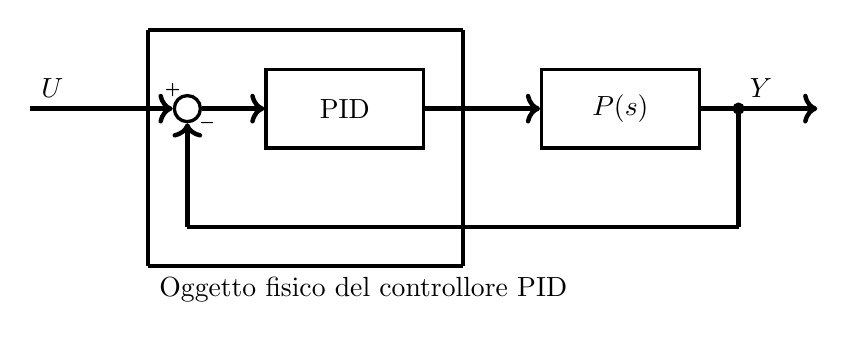
\begin{tikzpicture}[scale=2]
    \node[sum](sum)at(-1,0){};
    \draw[->,ultra thick](-2,0)node[above right]{$U$}--(sum.180)node[above]{$\scriptscriptstyle\boldsymbol{+}$};
    \node[block, right of=sum, node distance=2cm](c){PID};

    \draw[-,ultra thick](0.75,0.5)--(0.75,-1);
    \draw[-,ultra thick](0.75,0.5)--(-1.25,0.5);
    \draw[-,ultra thick](0.75,-1)--(-1.25,-1);
    \draw[-,ultra thick](-1.25,0.5)--(-1.25,-1)node[below right]{Oggetto fisico del controllore PID};

    \draw[->,ultra thick](sum.0)--(c.180);
    \filldraw[black](2.5,0)circle(1pt);

    \draw[->,ultra thick](2.5,0)node[above right]{$Y$}--(3,0);
    \draw[-,ultra thick](2.5,-0.75)--(2.5,0);

    %\node[block]at(0.75,-0.75)(h){$H(s)$};
    \node[block]at(1.75,0)(p){$P(s)$};

    \draw[-,ultra thick](p.0)--(2.5,0);
    \draw[->,ultra thick](c.0)--(p.180);

    %\draw[->,ultra thick](2.5,-0.75)--(h.0);
    %\draw[-,ultra thick](h.180)--(-1,-0.75);
    \draw[-,ultra thick](2.5,-0.75)--(-1,-0.75);
    \draw[->,ultra thick](-1,-0.75)--(sum.270)node[right]{$\scriptscriptstyle\boldsymbol{-}$};
\end{tikzpicture}\end{center}


Un controllore PID sarà quindi un 
oggetto avente funzione di trasferimento: $K_c+K_i\displaystyle\frac{1}{s}+K_ds$. Poiché un derivatore è un oggetto non causale, dipendendo da entrate future, si 
inserisce un polo lontano in un valore 
$\displaystyle\frac{1}{\varepsilon}$, per $\varepsilon$ arbitrariamente piccolo, in modo che risenta del polo solo per valori molto alti. Per cui la parte derivativa sarà: 
$\displaystyle\frac{K_ds}{s\varepsilon+1}$, si può esprimere come: 
$\displaystyle\frac{K_ds}{s\varepsilon+1}\frac{\displaystyle\frac{1}{s\varepsilon}}{\displaystyle\frac{1}{s\varepsilon}}=\frac{K_dN}{1+\displaystyle\frac{N}{s}}$, dove 
$N$ rappresenta un valore arbitrariamente grande. Un controllore PID può essere espresso, esplicitando il suo guadano come: 
\begin{equation}
    PID(s)=K_p\left(1+K_i\displaystyle\frac{1}{s}+K_d\frac{N}{1+\displaystyle\frac{N}{s}}\right)
\end{equation}
Per costruire un derivatore si considera: 

\begin{center}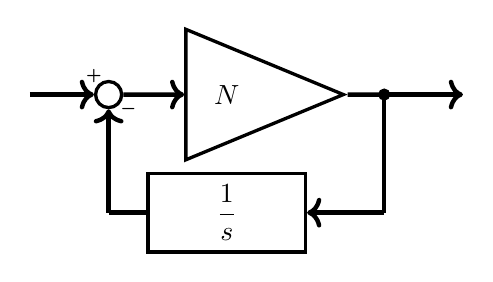
\begin{tikzpicture}[scale=2]
    \node[sum](sum)at(-1,0){};
    \draw[->,ultra thick](-1.5,0)--(sum.180)node[above]{$\scriptscriptstyle\boldsymbol{+}$};
    \node[triangle, right of=sum, node distance=1.5cm](g){$N$};
    \draw[->,ultra thick](sum.0)--(g.180);
    \draw[-,ultra thick](g.0)--(0.75,0);
    \filldraw[black](0.75,0)circle(1pt);
    \draw[->,ultra thick](0.75,0)--(1.25,0);
    \draw[-,ultra thick](0.75,-0.75)--(0.75,0);
    \node[block, below of=g, node distance=1.5cm](h){$\displaystyle\frac{1}{s}$};
    \draw[->,ultra thick](0.75,-0.75)--(h.0);
    \draw[-,ultra thick](h.180)--(-1,-0.75);
    \draw[->,ultra thick](-1,-0.75)--(sum.270)node[right]{$\scriptscriptstyle\boldsymbol{-}$};
\end{tikzpicture}\end{center}

Quest'oggetto fisicamente realizzabile avrà una funzione a ciclo chiuso $W(s)=\displaystyle\frac{N}{1+\displaystyle\frac{N}{s}}$, per un guadadno sulla catena diretta 
tendente all'infinito $N\to\infty$, si avrà un derivatore puro. 


\clearpage 

\section{Ingressi di Tipo Sinusoidale}

Per degli ingressi del tipo $u(t)=sin(\omega t)$, si ipotizza che un processo $G(s)$ sia asintoticamente stabile, e quindi abbia un'uscita a regime permanente della stessa 
classe dell'ingresso, ovvero $y_p(t)=Asin(\Omega t)$. La risposta del sistema nel dominio di Laplace sarà data da: 
$Y_p(s)=G(s)\cdot\displaystyle\frac{\omega}{s^2+\omega^2}$, si potrà scomporre in poli residui come: $Y_p(s)=\displaystyle\frac{R}{s-j\omega}+\frac{R^*}{s+j\omega}$, i valori 
di $R$ potranno essere calcolati usando la formula dei poli residui: 
\begin{gather}
    R=\lim_{s\to j\omega}(s-j\omega)Y_p(s)=\lim_{s\to j\omega}(s-j\omega)G(s)\cdot\displaystyle\frac{\omega}{s^2+\omega^2}\\
    \lim_{s\to j\omega}\cancelto{1}{(s-j\omega)}G(s)\displaystyle\frac{\omega}{\cancelto{1}{(s-j\omega)}(s+j\omega)}\\
    R=\displaystyle\frac{G(j\omega)\omega}{2j\omega}=\frac{G(j\omega)}{2j}\\
    R^*=-\frac{G^*(j\omega)}{2j}
\end{gather}
La funzione $G(j\omega)$, può essere espressa in termini polari come:
\begin{gather}
    G(j\omega)=|G(j\omega)|e^{j\phase{G(j\omega)}}\\
    G^*(j\omega)=|G(j\omega)|e^{-j\phase{G(j\omega)}}
\end{gather}

Allora si potrà esprimere la risposta a regime permanente come:
\begin{gather}
    Y_p(s)=\displaystyle\frac{1}{2j}\left(\frac{G(j\omega)}{s-j\omega}-\frac{G^*(j\omega)}{s+j\omega}\right)\\
    y_p(y)=\displaystyle\frac{1}{2j}(G(j\omega)e^{j\omega t}-G^*(j\omega)e^{-j\omega t})\\
    \displaystyle\frac{1}{2j}\left(|G(j\omega)|e^{j\phase{G(j\omega)}}e^{j\omega t}-|G(j\omega)|e^{-j\phase{G(j\omega)}}e^{-j\omega t}\right)\\
    |G(j\omega)|\left(\displaystyle\frac{e^{j\left(\omega t+\phase{G(j\omega)}\right)}-e^{-j\left(\omega t+\phase{G(j\omega)}\right)}}{2j}\right)\\
    y_p(t)=|G(j\omega)|sin\left(\omega t+\phase{G(j\omega)}\right)
\end{gather}

La risposta è proporzionale al modulo $|G(j\omega)|$. Data una certa pulsazione si ha che la risposta si annulla, per poi diventare negativa, per cui non si può 
amplificare una frequenza all'infinito. 

\begin{center}
    \begin{tikzpicture}[scale=2]
        \draw[->](0,-0.5)--(0,2)node[right]{$y_p(t)$};
        \draw[->](-0.5,0)--(2,0)node[above]{$\omega$};

        \draw[-, very thick]plot[smooth, domain=0:1.5](\x,{(1.5-\x)^0.5});
        \node[below]at(1.5,0){$\omega_t$};
    \end{tikzpicture}
\end{center}

Quest'analisi coincide con una trasformata di Fuorier, poiché una trasformata di Fuorier non è altro che una trasformata di Laplace solamente sull'asse 
immaginario: \\$\displaystyle\mathscr{F}_-(g(t))=\int_{0}^{\infty}g(t)e^{-j\omega t}dt=\mathscr{L}_-(y_p(t))\bigg|_{s=j\omega}$, corrisponde ad un'analisi dei soli segnali periodici. 
Per analizzare il comportamento della risposta del sistema, si dovranno analizzare gli andamenti del modulo e della fase del processo rispetto ad una pulsazione $\omega$. 

\subsection{Diagrammi di Bode}

Per analizzare il modulo di una funzione $G(s)$, con un guadagno normalizzato:
\begin{equation}
    G(s)=K_g\displaystyle\frac{(s\tau_i+1)\ldots(s\tau_n+1)}{(s\tau_k+1)\ldots(s\tau_m+1)}
\end{equation}
Per facilitare l'analisi rispetto ad ogni polo della funzione si considera una scala logaritimica in Decbibel:
\begin{equation}
    \big|x\big|_{dB}=20\log_{10}|x|
\end{equation}
Il modulo in Decibel del guadagno della funzione $K_g$, risulterà una costante addittiva:
\begin{equation}
    \big|K_g\big|_{dB}=20\log_{10}|K_g|
\end{equation}
Per un valore di modulo $0dB$, corrisponderà un guadagno unitario. \\
Essendo il guadagno $K_g$, un numero reale, la sua fase dipenderà solamente dal suo segno per cui: 
\begin{equation}
    \phase{K_g}=
    \begin{cases}
        0^\circ,\: K_g>0\\
        -180^\circ,\:K_g<0
    \end{cases}
\end{equation}
Per i diagrammi di Bode vengono usati i gradi.\\

Si analizza un termine generico $(s\tau_i+1)$. Il suo modulo sarà:
\begin{gather}
    |j\omega\tau+1|=\sqrt{\omega^2\tau^2+1}
\end{gather}
Viene espresso in Decibel:
\begin{equation}
    20\log_{10}\left(\sqrt{\omega^2\tau^2+1}\right)=10\log_{10}(\omega^2\tau^2+1)
\end{equation}
Si traccie un andamento asintotico per $\omega>>p$, allora si avrà: $\omega^2\tau^2>>1$, il modulo potrà quindi essere approssimato come:
\begin{gather}
    10\log_{10}(\omega^2\tau^2+1)\approx20\log_{10}(\omega\tau)\\
    20(\log_{10}\omega+\log_{10}\tau),\:\log_{10}\omega>>\log_{10}\tau\\
    20(\log_{10}\omega+\log_{10}\tau)\approx20\log_{10}\omega
\end{gather}
Per $\omega<<p$, si avrà invece che $\omega^2\tau^2<<1$, per cui il modulo potrà essere approssimato come:
\begin{gather}
    20\log_{10}(\omega^2\tau^2+1)\approx20\log_{10}1=0
\end{gather}

Viene definto $\lambda=\log_{10}\omega$, per cui $|j\omega\tau+1|_{dB}\approx20\lambda$.

\begin{center}
    \begin{tikzpicture}[scale=2]
        \draw[->,thick](-1,0)--(2,0)node[above]{$\lambda$};
        \draw[->,thick](0,-0.5)--(0,2)node[right]{$|\:\cdot\:|_{dB}$};

        \filldraw[black](-0.3,0)circle(1pt);
        \draw[dashed](0.3,0.2)--(0.3,0)node[below]{$\displaystyle\frac{1}{\tau}+\varepsilon$};
        \filldraw[black](0.3,0.2)circle(1pt);

        \draw[-,ultra thick](-1,0)--(-0.3,0)node[below]{$\displaystyle\frac{1}{\tau}-\varepsilon$};
        \draw[-,ultra thick](0.3,0.2)--(2,0.85);
    \end{tikzpicture}
\end{center}

Questa approssimazione non è definita nell'intorno del polo 
$\displaystyle\frac{1}{\tau}$, per cui si considera l'andamento del modulo nell'intervallo $\left(\displaystyle\frac{1}{\tau}+\varepsilon,\frac{1}{\tau}\right)$ come 
$20\lambda$, mentre si considera nell'intervallo $\left(\displaystyle\frac{1}{\tau},\frac{1}{\tau}-\varepsilon\right)$ come $0$. Questa approssimazione ha un errore 
di circa $\pm6dB$, nell'intorno dello zero o del polo, chiamato punto di rottura, non rilevamente per quest'analisi.  

\begin{center}
    \begin{tikzpicture}[scale=2]
        \draw[->,thick](-1,0)--(2,0)node[above]{$\lambda$};
        \draw[->,thick](0,-0.5)--(0,2)node[right]{$|\:\cdot\:|_{dB}$};



        \draw[-,ultra thick](-1,0)--(-0.05,0)node[below]{$\displaystyle\frac{1}{\tau}$};
        \draw[-,ultra thick](-0.05,0)--(2,0.85);
    \end{tikzpicture}
\end{center}

Il modulo viene espresso rispetto a $\lambda$, ed aumenta linearmente all'aumentare di $\lambda$. Si vuole rappresentare rispetto alla pulsazione per cui si considera 
$\omega=10^{\lambda}$, il modulo quindi aumenta lineramente rispetto a incrementi esponenziali della pulsazione $\omega$. I diagrammi di Bode sarnno quindi rappresentati 
su una carta semi logaritimica, divisa in decadi, ed il modulo crescerà di $20dB$ ogni decade in caso di uno zero, mentre scenderà di $20dB$ in caso di un polo. \\

La fase di un termine generico aumenterà da un valore iniziale di $0^{\circ}$, per $\omega=0$, ed aumenterà fino a raggiungere asintoticamente un valore massimo di 
$90^{\circ}$. 

\begin{gather}
    \omega=0,\: j\omega\tau+1=1\Rightarrow\phase{1}=0^{\circ}\\
    \omega\to\infty,\:j\omega\tau+1\approx j\omega\Rightarrow\phase{j\omega}=90^{\circ}
\end{gather}

Per cui $\phase{(j\omega\tau+1)}\in[0^{\circ},90^{\circ})$, in caso si tratti di uno zero, mentre se si considera un polo si avrà: 

\begin{equation}
    \phase{\displaystyle\frac{1}{j\omega\tau+1}}=\left(\phase{1}-\phase{(j\omega\tau+1)}\right)\in(-90^{\circ},0^{\circ}]
\end{equation}

Si approsima il cambiamento di fase come se fosse lineare nell'intervallo $\left(\displaystyle\frac{0.1}{\tau},\frac{10}{\tau}\right)$. 
Quest'approssimazione presenta un'errore di $\pm6^{\circ}$. 

\begin{center}
    \begin{tikzpicture}[scale=2]
        \draw[->](-1,0)--(2,0)node[above right]{$\omega$};
        \draw[->](-1,-1.5)--(-1,1.5)node[right]{$\phase{\:\cdot}$};

        \draw[-,ultra thick](-1,0)--(0.5,0)node[below]{$\displaystyle\frac{0.1}{\tau}$};
        \draw[-,ultra thick](0.5,0)--(1.5,1);
        \draw[-,ultra thick](1.5,1)--(2,1);
        \draw[dashed](1.5,1)--(1.5,0)node[below]{$\displaystyle\frac{10}{\tau}$};
        \draw[dashed](-1,1)node[left]{$90^{\circ}$}--(1.5,1);
        \node[left]at(-1,-1){$-90^{\circ}$};
        \draw[dashed](1,0.5)--(1,0)node[below]{$\displaystyle\frac{1}{\tau}$};

    \end{tikzpicture}
\end{center}

Per uno zero in $0$, il modulo aumenterà di $20dB$ su tutto l'intervallo di $\omega$, partendo da $-\infty dB$, tagliando il diagramma di Bode per $\omega=1$. 
Avrà una fase costante pari a $90^{\circ}$. \\
Per un polo in $0$, il modulo diminuirà di $20dB$ ogni decade partendo da $+\infty dB$, ed avrà una fase costante di $-90^{\circ}$. Si tratterà di un oggetto 
al limite di stabilità. 

\begin{center}
    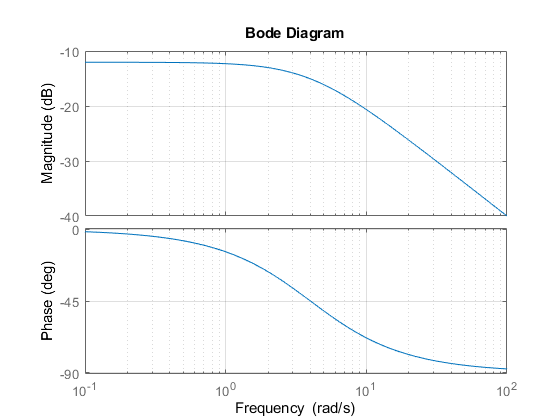
\includegraphics[width=10cm]{Bode1Polo}
\end{center}

Si considera un trinomio $\displaystyle\frac{s^2}{\omega_n^2}+\frac{2\xi s}{\omega_n}+1\to_{s=j\omega}-\frac{\omega^2}{\omega_n^2}+\frac{2\xi\omega}{\omega_n}j+1$. 
Per $\omega>>\omega_n$ il modulo sarà: 
\begin{gather}
    \left|-\frac{\omega^2}{\omega_n^2}+\frac{2\xi\omega}{\omega_n}j+1\right|=20\log{10}\left(\sqrt{\left(1-\displaystyle\frac{\omega^2}{\omega_n}^2\right)^2+\frac{4\xi^2\omega^2}{\omega_n^2}}\right)\\
    10\log_{10}=\left(4\xi^2\displaystyle\frac{\omega^2}{\omega_n^2}+\frac{\omega^4}{\omega_n^4}\right)\approx40\log_{10}\left(\displaystyle\frac{\omega}{\omega_n}\right)
\end{gather}
Per $\omega<<\omega_n$ il modulo sarà nullo, poiché: 
\begin{equation}
    20\log{10}\left(\sqrt{\left(1-\displaystyle\frac{\omega^2}{\omega_n}^2\right)^2+\frac{4\xi^2\omega^2}{\omega_n^2}}\right)\approx201log_{10}(1)=0
\end{equation}
Per $\omega=\omega_n$, il modulo dipenderà dallo smorzamento dei poli:
\begin{gather}
    20\log{10}\left(\sqrt{\left(1-\displaystyle\frac{\omega^2}{\omega_n}^2\right)^2+\frac{4\xi^2\omega^2}{\omega_n^2}}\right)=20\log_{10}(2\xi),\:\xi\in[0,1]\\
    20\log_{10}(2\xi)\in(-\infty,20\log_{10}(2)]
\end{gather}
Per uno smorzamento nullo sarà presenta un asintoto verticale per un valore di $\omega=\omega_n$, se non fosse uguale, allora il diagramma di Bode del modulo presenterebbe 
un affossamento nell'intorno di $\omega_n$, la cui profondità aumenta all'aumentare dello smorzamento. Questo affossamento è ciò che causa per i poli il fenomeno della 
risonanza, dove per una certa pulsazione si avrà un guadagno maggiore del guadagno statico del sistema. Per gli zeri si verifica il fenomeno dell'antirisonanza, dove 
per una certa pulsazione risulta estremamente attenuata. La sovraelongazione è un effetto dello smorzamento e sarà massima per smorzamento massimo. \\
Viene definito modulo alla risonanza $M_r$ la distanza tra il picco di risonanza ed il guadadno statico del sistema. 

\begin{center}
    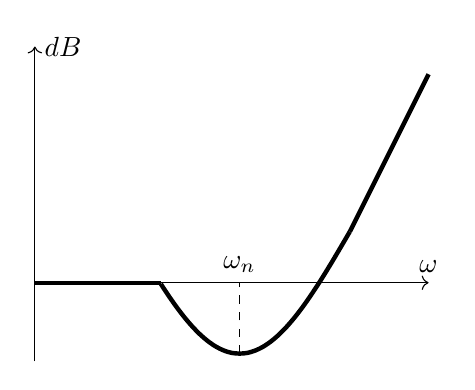
\begin{tikzpicture}[scale=2]
        \draw[->](-1,0)--(1.5,0)node[above]{$\omega$};
        \draw[->](-1,-0.5)--(-1,1.5)node[right]{$dB$};
        \draw[-,ultra thick](-1,0)--(-0.2,0);
        \draw[-, ultra thick]plot[smooth, domain=-0.2:1](\x,{1.55-2*e^-(\x-0.3)^2});
        \draw[dashed](0.3,-0.45)--(0.3,0)node[above]{$\omega_n$};
        \draw[-,ultra thick](1,0.324)--(1.5,1.324);
    \end{tikzpicture}
\end{center}

Per $\omega=0$, a fase del trinomio sarà: $\phase{(1)}=0^{\circ}$, mentre per $\omega\to\infty$, si avrà una fase tendente asintoticamente a: 

\begin{equation}
    \phase{\left(-\displaystyle\frac{\omega^2}{\omega_n^2}+2\xi\frac{\omega}{\omega_n}j+1\right)}\to\phase{-\displaystyle\frac{\omega^2}{\omega_n^2}}=-180^{\circ}
\end{equation}
Mentre per $\omega=\omega_n$, la fase sarà: 
\begin{equation}
    \phase{2\xi j}=90^{\circ}
\end{equation}
Quindi avverrà un cambiamento di fase nell'intorno di $\omega_n$, il cambiamento sarà sempre più rapido per smorzamenti sempre più piccoli, fino a presentare una 
discontinuità per smorzamenti nulli. Per smorzamenti sempre più piccoli la curva nel diagramma di Bode apparirà sempre più schiacciata. 
Nei sistemi causali ci saranno sempre più poli che zeri, per cui i loro diagrammi di Bode tenderanno sempre a scendere. \\

\begin{center}
    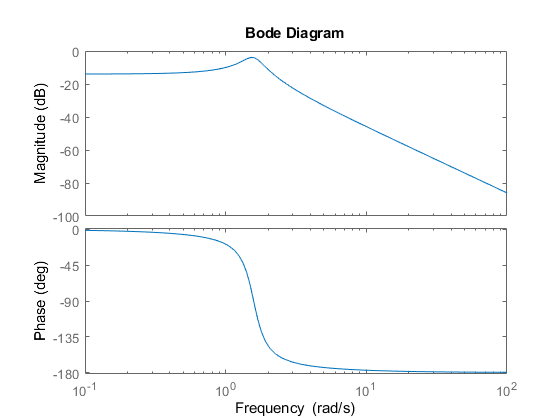
\includegraphics[width=10cm]{BodeRisonanza}
\end{center}

\subsection{Diagramma di Nyquist}
Data una funzione di trasferimento $M(s)=\displaystyle\frac{s-a}{s-b}$. Si definisce una qualsiasi curva chiusa $\mathbf{G}$ sul piano, e un punto $s$ che percorre la curva in senso 
orario. Allora per uno spostamento di $s$, comporterà uno spostamento di $M(s)$ nel piano di Gauss. 

\begin{center}
    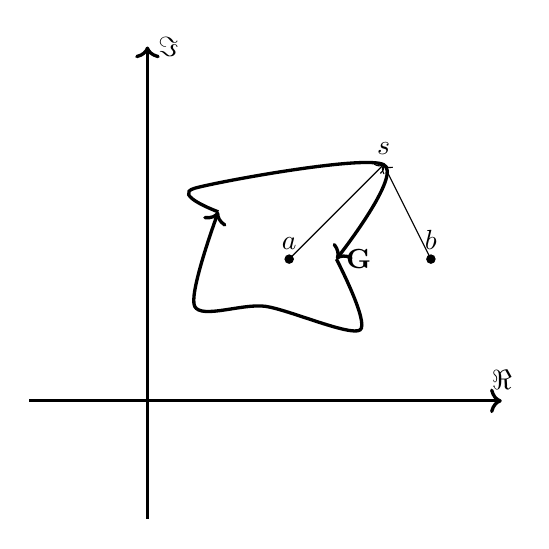
\begin{tikzpicture}[scale=3]
        \draw[->,very thick](0,-0.5)--(0,1.5)node[right]{$\Im$};
        \draw[->,very thick](-0.5,0)--(1.5,0)node[above]{$\Re$};

        \draw[->,very thick]plot[smooth]coordinates{(0.3,0.8) (0.2,0.9) (1,1) (0.8,0.6)};
        \draw[->,very thick]plot[smooth]coordinates{(0.8,0.6) (0.9,0.3) (0.5,0.4) (0.2,0.4)(0.3,0.8)};

        \node[right]at(0.8,0.6){$\mathbf{G}$};

        \node[above]at(1,1){$s$};
        \node[above]at(0.6,0.6){$a$};
        \filldraw[black](0.6,0.6)circle(0.5pt);
        \node[above]at(1.2,0.6){$b$};
        \filldraw[black](1.2,0.6)circle(0.5pt);
        
        \draw[->](0.6,0.6)--(1,1);
        \draw[->](1.2,0.6)--(1,1);
    \end{tikzpicture}
\end{center}

Per determinare se lo spostamento effettuato da $M(s)$ nel piano di Gauss a seguito di una variazione di $s$ formi una curva chiusa, si analizza il cambiamento di 
fase $\phase{M(s)}$. Se il cambiamento di fase della funzione rispetto ad $s$ è nullo allora la curva non ruota attorno all'origine, è un multiplo di $2\pi$: $2k\pi$ 
allora la curva ha ruotato $k$ volte attorno all'origine. Per determinare il cambiamento di fase: 

\begin{equation}
    \phase({M(s)})=\phase{s-a}-\phase{s-b}\\
\end{equation}

Poiché $s$ ruota attorno allo zero $a$, mentre non ruota attorno al polo $b$, il cambiamento di fase $\phase{s-a}$ risulta essere uguale ad una rotazione completa, ovvero 
$2\pi$, mentre $\phase{s-b}=0$ poiché la curva non ruota attorno a $b$. In base alla fase di $\vec{as}$ e $\vec{bs}$ si può ottenere il cambiamento di fase della funzione 
di trasfermento iniziale. Se un punto $s$ ruota intorno ad uno zero od un polo, la fase del vettore distanza $\vec{\alpha s}$ aumenterà fino a $k$-volte le rotazioni 
attorno a quello zero o polo. Si avrà quindi in questo caso:

\begin{equation}
    \phase{M(s)}=2\pi+0
\end{equation}

Quindi la funzione $M(s)$ ruoterà attorno all'origine. 

\begin{center}
    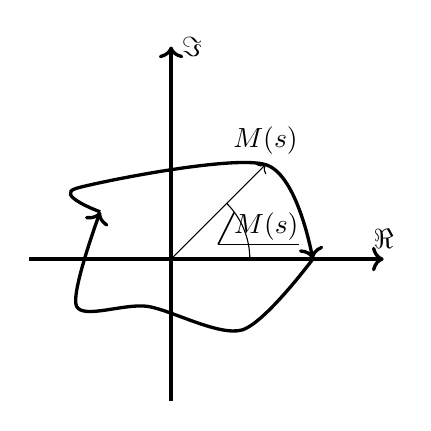
\begin{tikzpicture}[scale=3]
        \draw[->, very thick](0,0.6)--(1.5,0.6)coordinate(x)node[above]{$\Re$};
        \draw[->, very thick](0.6,0)--(0.6,1.5)node[right]{$\Im$};

        \draw[->,very thick]plot[smooth]coordinates{(0.3,0.8) (0.2,0.9) (1,1) (1.2,0.6)};
        \draw[->,very thick]plot[smooth]coordinates{(1.2,0.6) (0.9,0.3) (0.5,0.4) (0.2,0.4)(0.3,0.8)};

        \draw[->](0.6,0.6)coordinate(O)--(1,1)coordinate(M)node[above]{$M(s)$};
        \pic["$\phase{M(s)}$",draw, angle eccentricity=1.2, angle radius=1cm]{angle=x--O--M};
    \end{tikzpicture}
\end{center}

Gli unici termini che contribuiscono al cambiamneto di fase di $M(s)$ sono gli elementi interni alla curva. Poiché il cambiamneto di fase sarà sempre un numero intero di 
rotazioni complete intorno all'origine del piano di Gauss. Si definisce l'indicatore logaritimico $R_{M,0}$, che rappresenta il numero di queste rotazioni. Risulterà 
essere dato da:

\begin{equation}
    R_{M,0}=\#zeri_{\in \mathbf{G}}[M(s)]-\#poli_{\in \mathbf{G}}[M(s)]
\end{equation}

Tramite questo indicatore è possibile determinare graficamente la differenza poli-zeri di una qualsiasi funzione di trasfermineto in $s$. 

Dato un sistema controreazionato, avente una funzione a ciclo aperto $F(s)$, ed una funzione a ciclo chiuso 
$W(s)=\displaystyle\frac{F(s)}{1+F(s)}=1+\frac{N(s)}{D(s)}=\frac{D(s)+N(s)}{D(s)}$. 

\begin{center}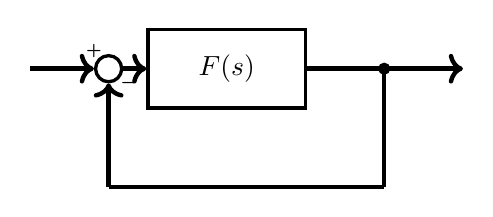
\begin{tikzpicture}[scale=2]
    \node[sum](sum)at(-1,0){};
    \draw[->,ultra thick](-1.5,0)--(sum.180)node[above]{$\scriptscriptstyle\boldsymbol{+}$};

    \node[block, right of=sum, node distance=1.5cm](g){$F(s)$};

    \draw[->,ultra thick](sum.0)--(g.180);
    \draw[-,ultra thick](g.0)--(0.75,0);
    \filldraw[black](0.75,0)circle(1pt);

    \draw[->,ultra thick](0.75,0)--(1.25,0);
    \draw[-,ultra thick](0.75,-0.75)--(0.75,0);
    \draw[-,ultra thick](0.75,-0.75)--(-1,-0.75);

    \draw[->,ultra thick](-1,-0.75)--(sum.270)node[right]{$\scriptscriptstyle\boldsymbol{-}$};
\end{tikzpicture}\end{center}

I poli della funzione a ciclo chiuso corrispodono ai poli di $F$. \\
Applicando il teoroma dell'indicatore logaritimico su $1+F(s)$, si traccia il percorso di Nyquist, una curva chiusa che contiene tutti gli oggetti aventi parte reale 
positiva. La curva si trova interamente sull'asse immaginario, la chiusura avviene all'infinito, per cui la risposta armonica corrisponde al percorso di Nyquist. 

\begin{center}
    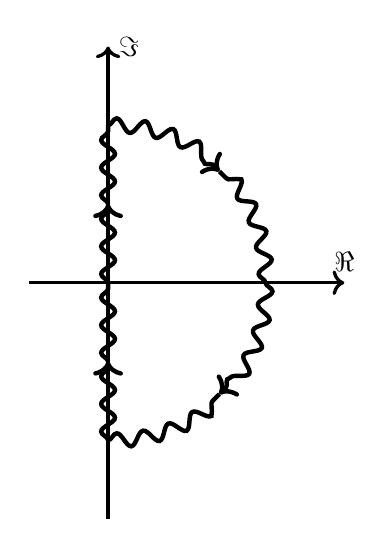
\begin{tikzpicture}[scale=2]
        \draw[->,very thick](-0.5,0)--(1.5,0)node[above]{$\Re$};
        \draw[->,very thick](0,-1.5)--(0,1.5)node[right]{$\Im$};

        \draw[->,snake it, ultra thick](0,-1)--(0,-0.5);
        \draw[-,snake it, ultra thick](0,-0.5)--(0,-0);
        \draw[->,snake it, ultra thick](0,0)--(0,0.5);
        \draw[-,snake it, ultra thick](0,0.5)--(0,1);
        
        \draw[->, snake it, ultra thick](0,1)arc(90:45:1cm);
        \draw[-, snake it, ultra thick](1,0)arc(0:45:1cm);       
        \draw[->, snake it, ultra thick](1,0)arc(0:-45:1cm);
        \draw[-, snake it, ultra thick](0,-1)arc(-90:-45:1cm);

    \end{tikzpicture}
\end{center}

Per cui si ha: 

\begin{equation}
    R_{1+F,0}=\#zeri_{Nyq}[1+F(s)]-\#poli_{Nyq}[1+F(s)]
\end{equation}

Dato che $1+F(s)=\displaystyle\frac{N(s)+D(s)}{D(s)}$, e la funione a ciclo chiuso $W(s)=\displaystyle\frac{N(s)}{D(s)+N(s)}$, gli zeri della funzione $1+F(s)$ equivalgono ai 
poli della funzione a ciclo chiuso, e i poli della funzione $1+F(s)$ equivalgono agli zeri della funzione a ciclo aperto $F(s)$, per cui la differenza poli zeri è data da: 

\begin{equation}
    R_{1+F,0}=\#poli_{Nyq}[W(s)]-\#poli_{Nyq}[F(s)]
\end{equation}

Un sistema è stabile se tutti i poli della sua funzione di trasferimento hanno parte reale positiva, per se il sistema è stabile il numero di poli a parte reale positiva 
sarà nullo: $\#poli_{Nyq}[W(s)]=0$, allora il numero di rotazioni attorno al punto zero di $W(s)$ sarà dato dal solo numero dei poli di $1+F(s)$. Questa relazione è 
reciproca per cui si ha che:

\begin{equation}
    \#poli_{Nyq}[W(s)]=0:\mbox{ sistema stabile}\iff R_{1+F(s),0}=-\#poli_{Nyq}[1+F(s)]
\end{equation}

Traslando la curva di Nyquist di $-1$, si ottiene la risposta armonica della funzione a ciclo aperto $F(s)$. L'indicatore logaritmico di $1+F(s)$ attorno a $0$, quindi 
corrisponde all'indicatore logaritimico di $F(s)$ attorno a $-1$:

\begin{equation}
    R_{F(s),-1}=R_{1+F(s),0}=-\#poli_{Nyq}[F(s)]
\end{equation}

Tramite questa relazione è possibile analizzare il sistema molto più facilmente, poiché la funzione a ciclo aperto è più facilmente alterabile. Se la funzione a ciclo aperto 
è asintoticamente stabile, allora la funzione affinché la funzione a ciclo chiuso stia anch'essa stabile, è necessario e sufficiente che il grafico di $F(s)$ non ruoti 
intorno a $-1$. Questo grafico corrisponde alla risposta armonica della funzione $F(s)$, e viene definito diagramma di Nyquist. A partire dai dati sulla risposta armonica 
forniti dal diagramma di Bode è possibile realizzare il diagramma polare di Nyquist di $F(s)$.  \\

Poiché su un diagramma di Bode vengono rappresentati solo incrementi positivi di $\omega$, si ottiene solo una metà del diagramma di Nyquist. Considerando frequenze negative 
il modulo rimarrà invariato, mentre la fase sarà opposta. Per cui per il diagramma di Nyquist è simmetrico rispetto all'asse delle ascisse.\\

Se la fase di una funzione di trasferimento non scende al di sotto dei $-180^{\circ}$ allora non potrà mai girare intorno al punto $-1$, poiché il modulo tende sempre 
a $0$ per ogni funzione di trasferimento stabile, per $\omega\to\infty$ il diagramma tende asintoticamente verso l'origine. Il sistema sarà quindi stabile per ogni 
controllore proporzionale maggiore di zero, se invece si sceglie un $Kc$ minore di zero, il sistema sarà stabile fino a quando il diagramma di Nyquist non include il 
punto $-1$. Aumentando il guadagno il diagramma si espande o si comprime, mentre la fase rimane costante, per cui esiste un intervallo di guadagni negativi dove il 
diagramma non contenga il punto $-1$, di conseguenza il sistema è stabile in quell'intervallo. 

\begin{center}
    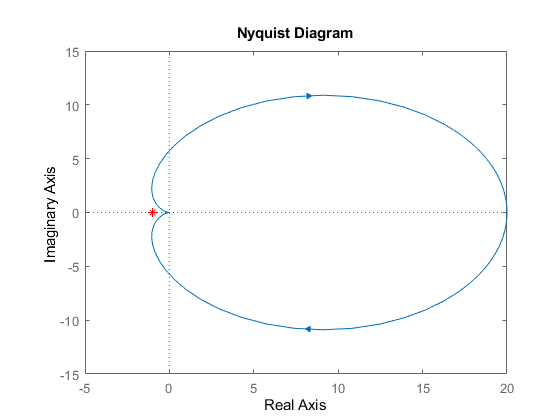
\includegraphics[width=6cm]{Nyquist2.png}
    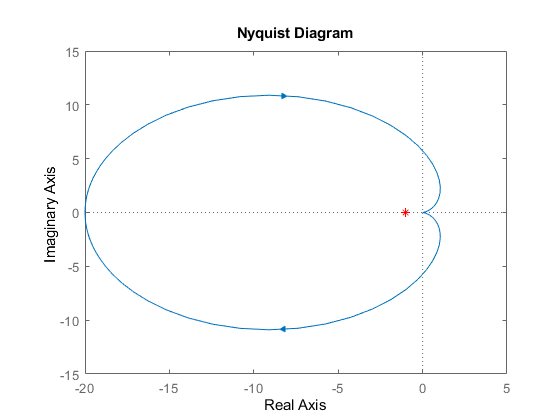
\includegraphics[width=6cm]{Nyquist1.png}
\end{center}

In caso la curva di Nyquist passi sopra un ad un polo, allora si considera un percorso uncinato in modo che $s$ gira intorno al polo $p$, questa rotazione attorno al polo 
causa una variazione di fase aggiuntiva di $+180^{\circ}$, il raggio di questa semicirconferenza è arbitrariamente piccolo, poiché deve escludere solo il punto coincidente 
con il polo. Può succedere per ogni polo immaginario puro, o per un polo nell'origine. 

\begin{center}
    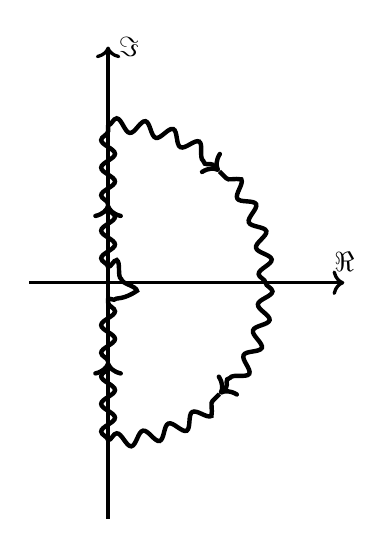
\begin{tikzpicture}[scale=2]
        \draw[->,very thick](-0.5,0)--(1.5,0)node[above]{$\Re$};
        \draw[->,very thick](0,-1.5)--(0,1.5)node[right]{$\Im$};

        \draw[->,snake it, ultra thick](0,-1)--(0,-0.5);
        \draw[-,snake it, ultra thick](0,-0.5)--(0,-0.1);
        \draw[->,snake it, ultra thick](0,0.1)--(0,0.5);
        \draw[-,snake it, ultra thick](0,0.5)--(0,1);

        \draw[-,snake it,ultra thick](0,0.1)arc(90:-90:0.1cm);
        
        \draw[->, snake it, ultra thick](0,1)arc(90:45:1cm);
        \draw[-, snake it, ultra thick](1,0)arc(0:45:1cm);       
        \draw[->, snake it, ultra thick](1,0)arc(0:-45:1cm);
        \draw[-, snake it, ultra thick](0,-1)arc(-90:-45:1cm);

    \end{tikzpicture}
\end{center}

In caso la fase cominci da $-90^{\circ}$ e raggiunga $-180^{\circ}$, il diagramma di Nyquist non completerà una curva chiusa, poiché tenderà ad essere parallelo all'asse 
immaginario per $\omega\to\pm\infty$. Si considera quindi una chiusura all'infinito in senso orario da $+90^{\circ}$ a $-90^{\circ}$, aggiungendo una variazione 
di fase di $-180^{\circ}$. Per cui sarà sempre stabile per controllori proporzionali maggiori di zero, mentre sarà instabile per valori di $K_c$ minori di zero, poiché 
la chiusura all'infinito considera tutti gli elementi con parte reale maggiore di zero, per valori negativi di $K_c$ comprenderà sicuramente il punto $-1$. 

\begin{center}
    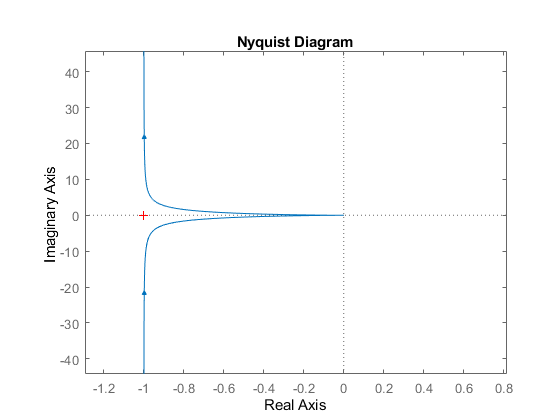
\includegraphics[width=8cm]{Nyquist3.png}
\end{center}

Se la fase parte da $-90^{\circ}$ e finisce a $-270^{\circ}$, il diagramma intersecerà l'asse delle ascisse in un punto negativo $\alpha$, potrebbe essere necessario comprimere 
il grafico con $K_c\in(0,K_{max})$, per allontanare il punto di intersezione da $-1$. 

\begin{center}
    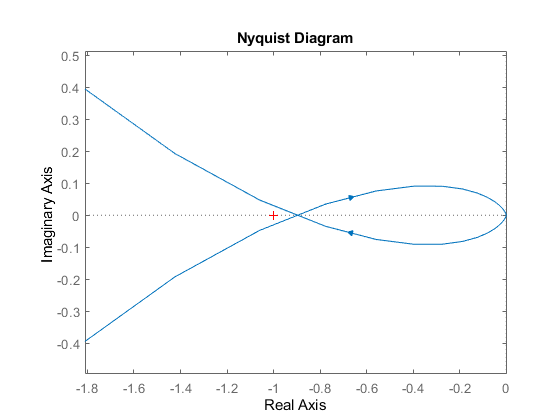
\includegraphics[width=8cm]{Nyquist4.png}
\end{center}

\subsection{Margini di Stabilità}

Viene definito questo guadagno massimo margine di guadagno $m_g$, il valore massimo per cui il modulo valga $-1$. 

\begin{equation}
    m_g\cdot\alpha\geq|-1|\Rightarrow m_g=\displaystyle\frac{1}{\alpha}
\end{equation}

dove $\alpha$ è il punto di intersezione del grafico con l'asse dei reali. Per un guadagno uguale al margine di guadagno, il sistema oscilla sul limite di stabilità, 
per valori di guadagno maggiore del maringe di guadagno il sistema ha dinamiche oscillatorie marcate. \\

Viene definito margine di fase $m_{\varphi}$, il massimo angolo di cui si può ruotare il diagramma di Nyquist prima di intersecare il punto $-1$. Ovvero la distanza del diagramma di Bode 
della fase da $-180^{\circ}$, per $\omega=\omega_t$, dove $\omega_t$ viene definita pulsazione di taglio per cui il modulo in decibel per quella frequenza è nullo. Rappresenta 
di quando si può sfasare il ciclo aperto. 

\begin{equation}
    m_{\varphi}=180^{\circ}-|\phase{F(j\omega_t)}|
\end{equation}


In caso si considerasse una funzione con zeri a parte reale positiva, bisogna calcolare i margini per ruotare abbastanza volte intorno al punto $-1$, non si calcolano 
direttamente dal diagramma di Bode. \\

Aumentando il guadagno, si diminuiscono gli errori a regime permanente e il tempo di salita, ma si diminuiscono i margini di stabilità, ciò destabilizza il sistema poiché è 
più suscettibile ad errori. Viene defintia robustezza di un sistema la sua capacità di resistere ad errori. Viene definita resilienza la capacità di un sistema di ritornare 
autonomamente allo stato di funzionomante in seguito a destabilizzazioni, è necessaria una "coscienza" del sistema per determinare se si trova in uno stato di funzionamento. \\

\subsection{Sistemi con Ritardo}

Per alcuni sistemi fisici è presente un ritardo nella misurazione dello stato del sistema, indotto da fenomeni intrinsechi al sistema o per esterni ad esso. 
Nel dominio del tempo un ritardo di tempo $\tau$ su un sistema $f(t)$ viene implementato come: $f(t-\tau)$, nel dominio della frequenza: 
$\mathscr{L}_-(f(t-\tau))=F(s)e^{-s\tau}$, per cui la funzione di trasferimento di un ritardo viene rappresentata come un esponenziale sulla catena di misura, prima del'oggetto 
di misurazione. 

\begin{center}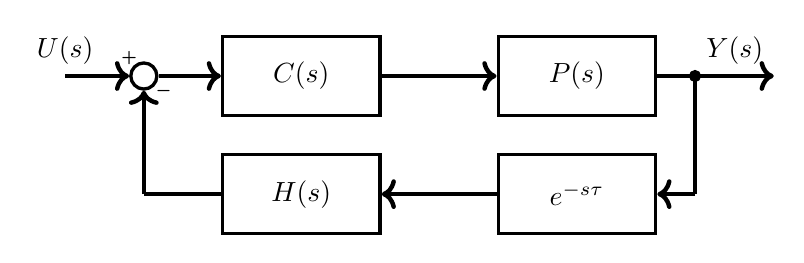
\begin{tikzpicture}[scale=2]

    \node[sum](sum)at(-1,0){};
    \draw[->,ultra thick](-1.5,0)node[above]{$U(s)$}--(sum.180)node[above]{$\scriptscriptstyle\boldsymbol{+}$};
    \node[block, right of=sum, node distance=2cm](c){$C(s)$};

    \draw[->,ultra thick](sum.0)--(c.180);
    \filldraw[black](2.5,0)circle(1pt);

    \draw[->,ultra thick](2.5,0)node[above right]{$Y(s)$}--(3,0);
    \draw[-,ultra thick](2.5,-0.75)--(2.5,0);

    \node[block]at(1.75,0)(p){$P(s)$};

    \draw[-,ultra thick](p.0)--(2.5,0);
    \draw[->,ultra thick](c.0)--(p.180);

    \node[block]at(0,-0.75)(h){$H(s)$};
    \node[block]at(1.75,-0.75)(e){$e^{-s\tau}$};
    
    \draw[->,ultra thick](2.5,-0.75)--(e.0);
    \draw[->,ultra thick](e.180)--(h.0);
    \draw[-,ultra thick](-1,-0.75)--(h.180);
    \draw[->,ultra thick](-1,-0.75)--(sum.270)node[right]{$\scriptscriptstyle\boldsymbol{-}$};

\end{tikzpicture}\end{center}

Il modulo del ritardo per una sinusoide in entrata sarà: $|e^{-\tau j\omega}|=1$, per cui avrà un modulo nullo in decibel, mentre la fase sarà: 
$\phase{e^{-\tau j\omega}}=-\tau\omega$. Per frequenze molto basse il ritardo non diminuisce la fase del sistema, per cui se il ritardo è troppo elevato o se il sistema 
opera su frequenze elevate può destabilizzare il sistema. 

\begin{center}
    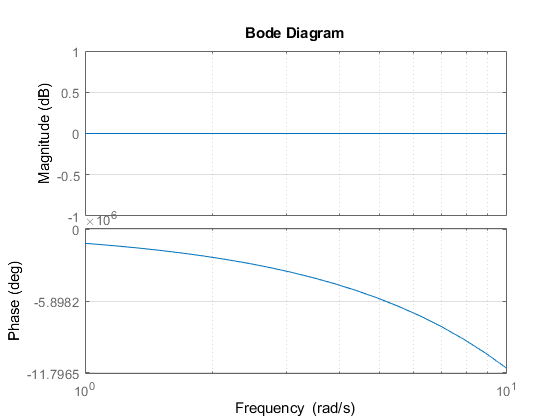
\includegraphics[width=12cm]{Bode2.png}
\end{center}

\subsection{Sistemi a Fase Non Minima}

Se il sistema presenta almeno uno zero a parte reale positiva, scomponendo l'uscita in fratti semplici rispetto ad un'enrata a gradino $\delta_{-1}(t)$, si avrà il residuo 
del gradino minore di zero, per un numero dispari di zeri a parte reale posisitiva. Il transitorio potrà avere una risposta nel transitorio opposto alla risposta a pieno regime. 

\begin{gather}
    Y(s)=\displaystyle\frac{R_0}{s}+\frac{R_1}{s\tau_1+1}+...+\frac{R_n}{s\tau_n+1},\:R_0<0\\
    y(t)=-|R_0|\delta_{-1}(t)+R_1e^{-\tau_1t}+...+R_ne^{-\tau_nt}
\end{gather}

\begin{center}
    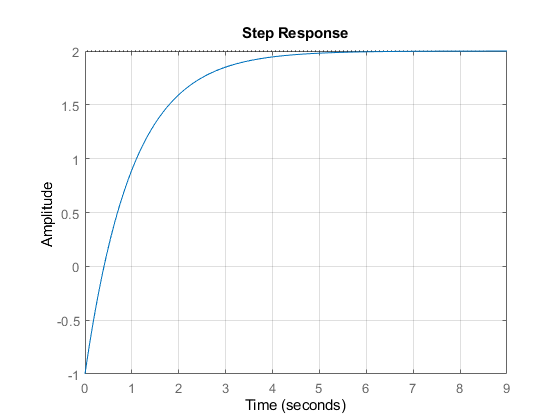
\includegraphics[width=10cm]{Step1.png}
\end{center}

\subsection{Sintesi Diretta}

Dato un sistema avente una funzione a ciclo chiuso $W(s)=\displaystyle\frac{C(s)P(s)}{1+C(s)P(s)}$, se si vuole ottenere una specifica funzione di trasferimento, si può 
calcolare direttamente un controllore $C(s)$ per ottenerla: 

\begin{gather}
    W(s)(1+C(sP(s)))=C(s)P(s)\\
    C(s)=\displaystyle\frac{1}{P(s)}\cdot\frac{W(s)}{1-W(s)}
\end{gather}

Se il processo $P(s)$ è causale, allora il suo inverso $\displaystyle\frac{1}{P(s)}$ non potrà essere causale, poiché presenterà più zeri che poli. Allora il controllore $C(s)$ 
potrà essere stabile solo se l'eccesso poli-zeri di $\displaystyle\frac{1}{P(s)}$ viene bilanciato da $1-W(s)=D(s)-N(s)$: 

\begin{equation}
    C(s)=\displaystyle\frac{1}{P(s)}\frac{N(s)}{D(s)-N(s)}
\end{equation}

Se si sceglie una funzione $W(s)$ asintoticamente stabile, allora il controllore cancella il processo, contenendo $\displaystyle\frac{1}{P(s)}$. Se il processo contiene zeri 
a parte reale positiva, allora il controllore contiene poli a parte reale positiva, analiticamente si cancellano, ma non si possono cancellare le dinamiche di un sistema.  
Per cui un sistema con un controllore ottenuto tramite sintesi diretta presenta delle dinamiche instabili, non è stabile internamente. 

\subsection{Guadagno}

Il guadagno ad anello oltre a diminuire l'errore di riproduzione di segnali di tipo $k$ e rigettare disturbi di tipo $k$, diminuisce la sensibilità diretta del 
sistema, ottenendo presetazioni più costanti. \\

\subsubsection{Sensibilità}

Viene definita la funzione sensibilità di una funzione $Q(\alpha)$, il rapporto tra le variazioni percentuali della funzione e della variabila indipendente:

\begin{equation}
    S_{\alpha}^Q:=\displaystyle\frac{\displaystyle\frac{dQ}{Q}}{\displaystyle\frac{d\alpha}{\alpha}}=\frac{\alpha}{Q}\frac{dQ}{d\alpha}
\end{equation}

Per un sistema a controreazione avente una funzione $G(s)$ in catena diretta ed una funzione $H(s)$ in catena di misura, si può considerare la sensibilità del sistema 
sia rispetto a $G(s)$ che rispetto a $H(s)$:

\begin{gather}
    S_H^W(s)=\displaystyle\frac{H}{W}\frac{dW}{dH}=-\frac{G(s)H(s)}{1+G(s)H(s)}\\
    S_G^W(s)=\displaystyle\frac{G}{W}\frac{dW}{dG}=\frac{1}{1+G(s)H(s)}
\end{gather}

La sensibilità del sistema rispetto alla funzione a $H(s)$ è complementare alla sensibiltà diretta del sistema rispetto a $G(s)$:

\begin{equation}
    S^W_G(s)-S^W_H(s)=1
\end{equation}

Se si considera una funzione $G(s,p)$ la sensibiltà del sistema rispetto ad una delle variabili indipendenti di $G$ è data da:

\begin{gather}
    S^W_p(s)=\displaystyle\frac{p}{W}\frac{dW}{dp}=\frac{p}{W}\frac{dW}{dG}\frac{dG}{dp}\left(\frac{G}{G}\right)\\
    \left(\frac{p}{G}\frac{dG}{dp}\right)\left(\frac{W}{G}\frac{dW}{dG}\right)\\
    S^W_p(s)=S^G_p(s)S^W_G(s)
\end{gather}

Considerando un sistema con un errore in catena diretta, si può calcolare l'effetto dell'errore sul sistema tramite la sensibilità diretta. Si considera l'uscita 
di un errore $d$:

\begin{equation}
    Y_d(s)=\displaystyle\frac{G_2(s)}{1+G_1(s)G_2(s)H(s)}D(s)=S^W_{G_1}(s)G_2(s)D(s)
\end{equation}

L'effetto dell'errore è direttamente proporzionale alla sensibilità diretta, per cui all'aumentare del gaudagno ad anello l'effetto dell'errore diminuisce.  
Se si considera un errore $h$ in catena di misura, non potrà essere alterato facilmente dal guadagno ad anello, per cui risulta più problematico. 

\begin{center}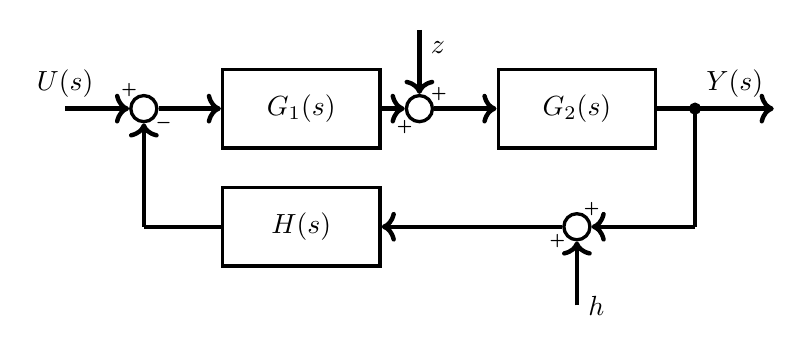
\begin{tikzpicture}[scale=2]
    \node[sum](sum)at(-1,0){};
    \node[sum](sum2)at(0.75,0){};
    \draw[->,ultra thick](-1.5,0)node[above]{$U(s)$}--(sum.180)node[above]{$\scriptscriptstyle\boldsymbol{+}$};


    \node[block, right of=sum, node distance=2cm](g){$G_1(s)$};
    \draw[->,ultra thick](sum.0)--(g.180);
    \draw[->,ultra thick](g.0)--(sum2.180)node[below]{$\scriptscriptstyle\boldsymbol{+}$};
    

    \filldraw[black](2.5,0)circle(1pt);


    \draw[->,ultra thick](0.75,0.5)node[below right]{$z$}--(sum2.90)node[right]{$\scriptscriptstyle\boldsymbol{+}$};

    \node[block]at(1.75,0)(k){$G_2(s)$};
    \draw[->,ultra thick](sum2.0)--(k.180);
    \draw[-,ultra thick](k.0)--(2.5,0);

    \draw[->,ultra thick](2.5,0)node[above right]{$Y(s)$}--(3,0);
    \draw[-,ultra thick](2.5,-0.75)--(2.5,0);

    \node[sum](sum3)at(1.75,-0.75){};
    \draw[->,ultra thick](2.5,-0.75)--(sum3.0)node[above]{$\scriptscriptstyle\boldsymbol{+}$};
    \draw[->,ultra thick](1.75,-1.25)node[right]{$h$}--(sum3.270)node[left]{$\scriptscriptstyle\boldsymbol{+}$};

    \node[block, below of=g, node distance=1.5cm](h){$H(s)$};
    \draw[->,ultra thick](sum3.180)--(h.0);
    \draw[-,ultra thick](h.180)--(-1,-0.75);

    \draw[->,ultra thick](-1,-0.75)--(sum.270)node[right]{$\scriptscriptstyle\boldsymbol{-}$};
\end{tikzpicture}\end{center}

\subsubsection{Amplificatori Operazionali}

Data una funzione di trasferimento a ciclo chiuso $W(s)=\displaystyle\frac{G(s)}{1+G(s)H(s)}$, si considera $H(s)=h$. Per il modulo della funzione a catena diretta molto alto: 

\begin{equation}
    |G(j\omega)|>>0\Rightarrow|W(j\omega)|=\displaystyle\frac{|G(j\omega)|}{|1+G(j\omega)h|}=\frac{1}{h}
\end{equation}

Quindi per guadagno ad anello molto elevato e basse frequenze la funzione a ciclo chiuso sarà l'inverso della funzione sulla catena di misura. \\

Un integratore è un operazionale descritto dal seguente circuito, in configurazione invertente:

\begin{center}
    \begin{circuitikz}
        \draw
        (-1,0) node[ground]{} to[short] ++(1,0)node[above left]{$v_X$}
        node[op amp, noinv input up, anchor=+](OA){$A$}
        (OA.-) -- ++(0,-1) coordinate(FB)
        to[R=$R$,*-o] ++(0,-2)node[right]{$v_{in}$}
        (FB) to[C=$C$, *-] (FB -| OA.out) -- (OA.out)
        to [short, *-o] ++(1,0) node[above]{$v_{out}$}
        ;
    \end{circuitikz}
\end{center}

Si definisce impedenza di un circuito il rapporto tra la tensione applicata ai capi del circuito e la corrente che vi ci scorre, nel dominio di Laplace, misura la facilità 
con cui una corrente alternata attraversa un circuito. Le impedenze 
derivano dalle tensioni generate dai vari oggetti di un circuito come un resistore, un capacitore ed un induttore: 

\begin{gather}
    Z_R:R=\displaystyle\frac{v(t)}{i(t)}\Rightarrow Z_R=\frac{V(s)}{I(s)}=R\\
    Z_C:v_{in}=\displaystyle\frac{1}{C}\int i\:d\tau\\
    \dot v_{in}=\displaystyle\frac{1}{C}i\\
    sV(s)_{in}=\frac{1}{C}I(s)\Rightarrow Z_C=\frac{1}{Cs}\\
    Z_L: v(t)=L\dot i(t)\\
    V(s)=sLI(s)\Rightarrow Z_L=sL
\end{gather}

Si definisce amplificatore operazionale un oggetto avente un guadagno elevato $K_A\approx10^5$ ed un'impedenza elevatissima in entrata proporzionale al suo guadagno, perciò si 
considera il caso dove l'entrata sia nulla. Si può quindi rappresentare in un sistema a bloccchi il circuito di un integratore operazionale:

\begin{center}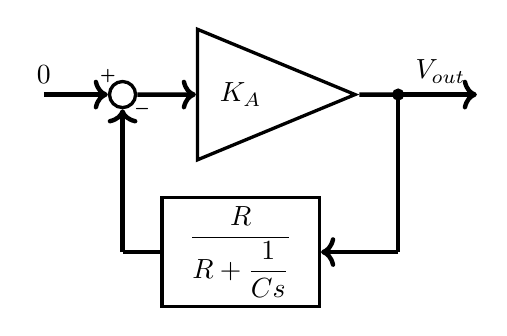
\begin{tikzpicture}[scale=2]
    \node[sum](sum)at(-1,0){};
    \draw[->,ultra thick](-1.5,0)node[above]{$0$}--(sum.180)node[above]{$\scriptscriptstyle\boldsymbol{+}$};
    \node[triangle, right of=sum, node distance=1.5cm](g){$K_A$};

    \draw[->,ultra thick](sum.0)--(g.180);
    \draw[-,ultra thick](g.0)--(0.75,0);
    \filldraw[black](0.75,0)circle(1pt);

    \draw[->,ultra thick](0.75,0)--(1.25,0)node[above left]{$V_{out}$};
    \draw[-,ultra thick](0.75,-1)--(0.75,0);
    \node[block, below of=g, node distance=2cm](h){$\displaystyle\frac{R}{R+\displaystyle\frac{1}{Cs}}$};

    \draw[->,ultra thick](0.75,-1)--(h.0);
    \draw[-,ultra thick](h.180)--(-1,-1);
    \draw[->,ultra thick](-1,-1)--(sum.270)node[right]{$\scriptscriptstyle\boldsymbol{-}$};
\end{tikzpicture}\end{center}

Poiché il guadagno $K_A$ è molto elevato, si può approssimare la funzione a ciclo chiuso come: 

\begin{equation}
    W(s)=\displaystyle\frac{R+\displaystyle\frac{1}{Cs}}{R}=\frac{RCs+1}{RCs}
\end{equation}

Rappresenta un integratore con uno zero in $-\displaystyle\frac{1}{RC}$, per un intervallo di frequenze può essere approssimato come un integratore puro. \\

Per ottenere un derivatore si considera invece un induttore al posto del resistore:

\begin{center}
    \begin{circuitikz}
        \draw
        (-1,0) node[ground]{} to[short] ++(1,0)node[above left]{$v_X$}
        node[op amp, noinv input up, anchor=+](OA){$A$}
        (OA.-) -- ++(0,-1) coordinate(FB)
        to[L=$L$,*-o] ++(0,-2)node[right]{$v_{in}$}
        (FB) to[C=$C$, *-] (FB -| OA.out) -- (OA.out)
        to [short, *-o] ++(1,0) node[above]{$v_{out}$}
        ;
    \end{circuitikz}
\end{center}

L'amplificatore presenta un comportamento non lineare, ma in controreazione ha un comportamento lineare; ha una risposta in frequenza che si può determinare 
sperimentalmente usando un generatore di funzioni in entrata ed un oscilloscopio in uscita. In ciclo aperto presenta una banda passante piccola, se si inserisce un 
fattore $\displaystyle\frac{1}{K_d}<1$ in controreazione aumenta la banda passante, ma diminuise il guadagno del sistema. Poiché un amplificatore è un oggetto a guadagno 
molto elevato, è possibile aumentare la banda passante considerevolmente senza disturbare di troppo le funzioni dell'amplificatore. 

\begin{center}
    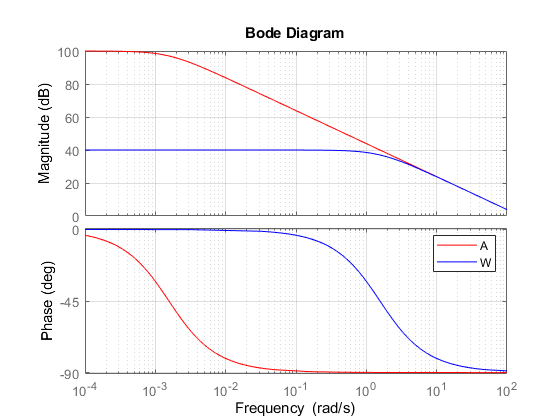
\includegraphics[width=10cm]{Amplificatore.png}
\end{center}

\subsubsection{Linearizzazione}

Un qualsiasi sistema non lineare definito da una funzione $f$, se messo in controreazione con un guadagno $K$, avrà una risposta: 

\begin{gather}
    \begin{cases}
        y=f(v)\\
        v=k(u-y)
    \end{cases}\\
    y=f(k(u-y))\\
\end{gather}

Dove $f(x)$ è una funzione non lineare, considerando un guadagno molto elevato $k>>0$, allora $y\propto u-y$, se il sistema non diventa stabile prima. \\
Un transistor è un oggetto non lineare, ma ha un guadagno molto elevato, per cui viene costruito in controreazione per avere comportamenti lineari. 

\subsection{Errore di Tipo Sinusoidale}

Si vuole determinare l'errore $\tilde{e}(t)=\tilde{y}_d-\tilde{y}(t)$ rispetto ad un riferimento ideale per un entrata sinusoidale $\tilde{u}(t)=sin(\tilde{\omega}t)$, di un'uscita 
$\tilde{y}(t)=Msin(\tilde{\omega}t+{\varphi}(\tilde{\omega}))$, dove $M(\tilde{\omega})=|W(j\omega)|_{\omega=\tilde{\omega}}$ e 
$\varphi(\tilde{\omega})=\phase{W(j\omega)}_{\omega=\tilde{\omega}}$. 
L'errore sarà dato da:

\begin{equation}
    W_e(s)=|Kd-W(j\omega)|=\left|\displaystyle\frac{Kd^2}{Kd+G(j\omega)}\right|=\left|\frac{Kd}{1+F(j\omega)}\right|
\end{equation}

Per un guadagno ad anello molto elevato si ha un errore piccolo: 
$|G(j\omega)|>>0\Rightarrow \tilde{e}(\omega)=\displaystyle\frac{Kd}{|F(j\omega)|}<<1$. Intorno alla pulsazione di taglio, si ha un guadagno ad anello basso, per cui si ha un errore 
$W_e(s)=Kd$. \\

\subsection{Carta di Nichols}

Tracciando il modulo della funzione a ciclo chiuso rispetto alla frequenza, si individuano il modulo alla risonanza $Mr$ definito come la distanza tra il guadagno statico 
ed il picco del modulo, se il modulo rispetto alla frequenza è strettamente decrescente, il modulo alla risonanza è nullo. Si definisce banda passante $\omega_{-3}$, la 
frequenza per cui il modulo della funzione a ciclo chiuso scende al di sotto di $-3\:dB$. Analogamente al tempo caratteristico, rappresenta la massima pulsazione trattata dal 
sistema prima che l'effetto dimnuisca considerevolmente. \\
La sovraelongazione $s$ è direttamente proporzionale al modulo alla risonanza $s\propto Mr$, il tempo di salita $t_s$ e la banda passante sono circa inversamente proporzionali 
$t_s\cdot\omega_{-3}\approx cost.$. Per un aumento del guadagno, aumentano sia la banda passante che la pulsazione di taglio, per cui le due frequenze sono direttamente proporzionali, 
mentre diminuisce il tempo di salita, per cui $\omega_t\propto\omega_{-3}\cdot t_s$.

\begin{center}
    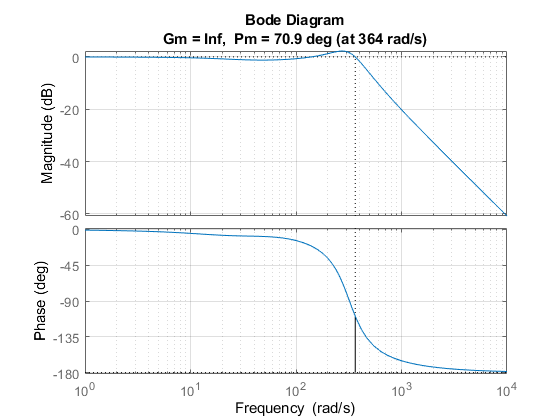
\includegraphics[width=10cm]{Bode3.png}
\end{center}

La carta di Nichols è un diagramma che rappresenta l'andamento della fase e del modulo di una funzione di trasferimento. Considera la fase nell'intervallo 
$[-360^{\circ},0^{\circ}]$, ed il modulo in $[-80\:dB, 40\:dB]$, viene usato un sistema di coordinate rettilineo usato per la funzione a ciclo aperto. Mentre per la funzione 
a ciclo chiusco si usa un sistema di coordinate curvilineo, formato da luogo delle curve a modulo costante, fino a $-3dB$, ed a fase costante. Ovvero si considera o la fase 
o il modulo costante e si traccia l'andamento della funzione a ciclo chiuso $W=|W|e^{\phase{W}}$ per la variazione della rimanente. Ha l'origine nel punto 
$(0\:db,-180^{\circ})$: $-1$. \\

Data $W=\displaystyle\frac{F}{1+F}$, ci si può ricavare la funzione a ciclo aperto: $F=\displaystyle\frac{W}{1-W}$. Si ricava il modulo della funzione a ciclo chiuso in 
una data fase dall'intersezione della curva a modulo costante con la funzione a ciclo aperto. Per $|W|_{dB}=-20\:dB$, le curve a modulo costante sono quasi rettilinere nella 
carta di Nichols, per cui il comportamento della funzione a ciclo chiuso è molto simile alla funzione a ciclo aperto: 
$W=\displaystyle\frac{F}{1+\cancelto{\approx0}{F}}\approx F$. \\

Dall'intersezione di $F$ con la curva di modulo $-3\:dB$ si può determinare il valore della banda passante $\omega_{-3}$, dalla fase corrispondente all'intersezione. La 
distanza sull'asse a $0:dB$ della curva $F$ dall'origine rappresenta il margine di fase $m_{\varphi}$, mentre la distanza sull'asse a $-180^{\circ}$ della curva dall'origine 
rappresenta il margine di guadagno $m_g$. Per questo curve che passano l'asse a $0\:dB$ da destra avranno una funzione a ciclo chiuso stabile. Il modulo alla risonanza è la 
curva a modulo costante maggiore che interseca la funzione a ciclo aperto, per $K_d=1$. Per un modulo alla risonanza maggiore, la funzione $F$ si avvicina all'origine della 
carta di Nichols, dimnuendo il margine di fase, per cui $Mr\propto\displaystyle\frac{1}{m_{\varphi}}$; il fenomeno della risonanza è presente per $m_{\varphi}<<1$. 

Dalle relazioni ottenute precedentemente: 
\begin{equation}
    \begin{cases}
        s\propto Mr\propto\displaystyle\frac{1}{m_{\varphi}}\\
        t_s\cdot\omega_{-3}\propto\omega_t
    \end{cases}
\end{equation}

\begin{center}
    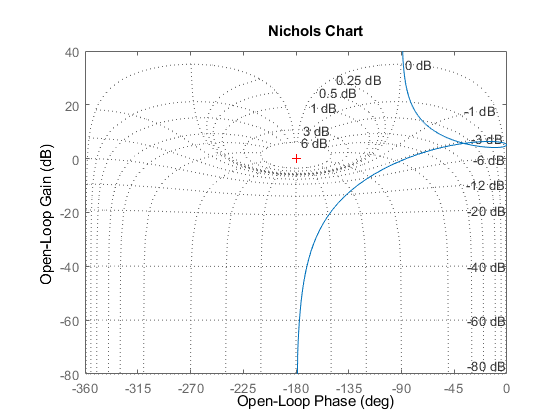
\includegraphics[width=10cm]{Nichols1.png}
\end{center}

\subsection{Reti Corretrici}

Per modificare in maniere selettiva l'andamento di un sistema si agisce direttamente sui poli e gli zeri del sistema. Un metodo per eliminare una dinamica sfavorevole per 
introdurne un'altra consiste nell'inserire una funzione in catena diretta contente una coppia polo-zero a guadagno unitario. In questo modo si mantiene il guadagno statico 
del sistema e si agisce direttamente sull'andamento di Bode del processo. Questo metodo non si può utilizzare per eliminare elementi instabili da un processo, poiché le 
dinamiche di un sistema anche se vengono cancellate analiticamente rimangono fisicamente in esso. Per questo motivo anche il controllore deve avere una coppia poli-zeri 
stabile. \\

Un controllore di questo tipo viene chiamato rete correttrice $R(s)$, può presentare il polo prima dello zero, in questo caso si chiama rete attenuatrice, oppure il polo 
dopo lo zero, rete anticipatrice. Le reti correttrici vengono definite da un parametro $m$, che rappresenta la distanza tra il polo e lo zero nel tempo, e di conseguenza 
l'intensità del cambiamento che provoca la rete, più i poli sono vicini, più l'effetto della rete viene diminuito poiché più sono vicini, meno tempo ha l'altra dinamica 
per bilanciare la prima. Queste reti vengono costruite fisicamente tramite una serie di resistenze ed un condensatore, più la coppia polo-zero è distante più precisione sarà richiesta per le 
resistenze, per cui si tende a scegliere tra reti a partià di effetto, quella con un parametro $m$ minore per diminuire il costo di produzione del componente fisico. \\

Le reti correttrici sono definite da un altro parametro $\tau$, utilizzato per traslare globalmente la coppia polo-zero, per un aumento o diminuzione dell'effetto 
causato della rete. Questo effetto viene indicato su un diagramma di Bode rispetto ad una frequenza $\omega$, pari alla frequenza dove si vuole applicare la rete tenendo 
conto della traslazione della coppia polo-zero $\tau$. Poiché si vuole agire sulla pulsazione di taglio si avrà una frequenza $\omega=\omega_t\cdot\tau$. 

Le reti hanno funzione di trasferimento: 

\begin{gather}
    R(s)_{antp.}=\displaystyle\frac{1+\tau s}{1+\displaystyle\frac{\tau}{m}s}\\
    R(s)_{att}=\displaystyle\frac{1+\displaystyle\frac{\tau}{m}s}{1+\tau s}
\end{gather}

In una rete anticipatrice, presentando uno zero prima del polo, i moduli saliranno per poi rimanere costanti dopo il polo, mentre le fasi saliranno e poi scenderanno. Essendo 
una attenuatrice l'esatto opposto, i moduli prima scenderanno prima di arrestarsi e le fasi prima scenderanno e poi saliranno. 
\'{E} possibile che una rete correttrice si trovi al limite di stabilità. \\

Il diagramma usato per calcolare una rete si chiama carta delle reti compensatrici: 

\begin{center}
    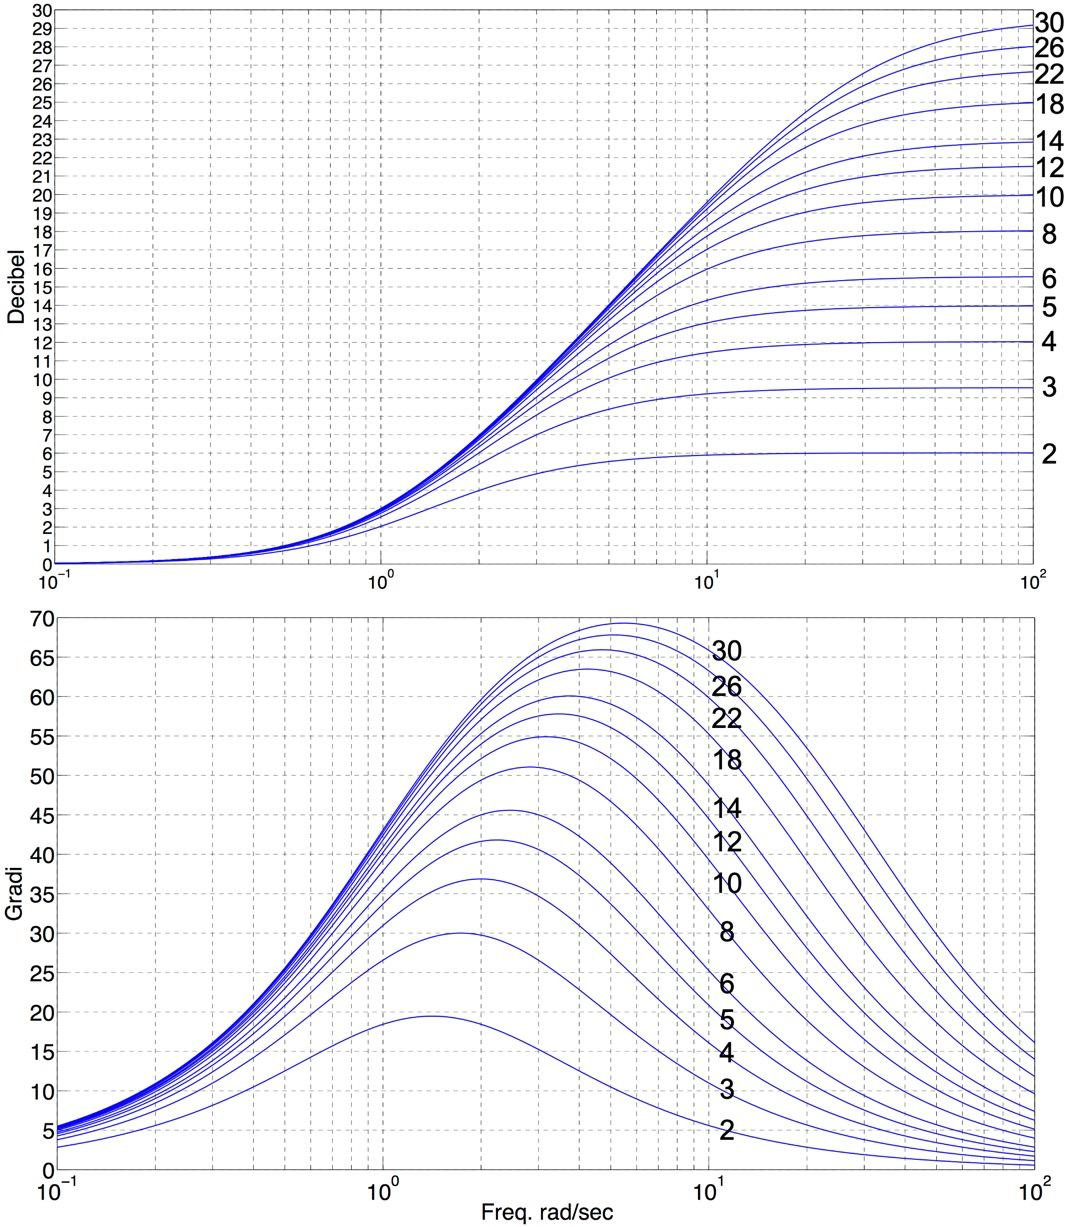
\includegraphics[width=10cm]{CartaReti.jpg}
\end{center}

Poiché per una rete attenuatricie, l'effetto causato è esattamente l'opposto di una anticipatrice, si usa sempre la stessa carta per entrambe le reti, solo si considera 
l'effetto negativo quando si tratta di una attenuatrice. \\

In un sistema generico, la rete correttrice viene aggiunta in catene diretta al controllore $C(s)$, che presenta un numero $h$ di integratori ed un guadagno $K_c$, per cui 
il controllore del sistema diventa: 

\begin{equation}
    C(s)=\displaystyle\frac{K_c}{s^h}\cdot R(s)
\end{equation}

Si può dividere l'effetto di una rete, per qualsiasi $m$, in due zone. In una prima zona, il modulo varia di poco, mentre cambia notevolmente la fase, questo può essere 
usato in sistemi al limite di stabilità per recuperare margine di fase, senza cambiare il modulo del sistema. In una seconda zona si può variare di molto il modulo del 
sistema senza intaccare di troppo la fase. Per stabilizzare un sistema è necessario un margine di fase abbastanza grande per resistere ad errori, per cui si scelgono sempre 
reti che a parità di modulo diminuiscano il meno possibile la fase. \\


Si possono combinare più reti per sistemi, dove ogni rete agisce in un punto diverso nel tempo, in questo caso si useranno parametri $\tau$ e $m$ diversi per ogni singola 
rete nel controllore. 

%Reti in circuiti: 




%circuitikz

\subsection{Rumori Aleatori}

Dei rumori aleatori sono dei tipi di errori che agiscono su un sistema il cui comportamento può essere descritto solo 
statisticamente. Per rigettare questo tipo di errori, si analizza l'intervallo di frequenze su cui agiscono. 

\begin{center}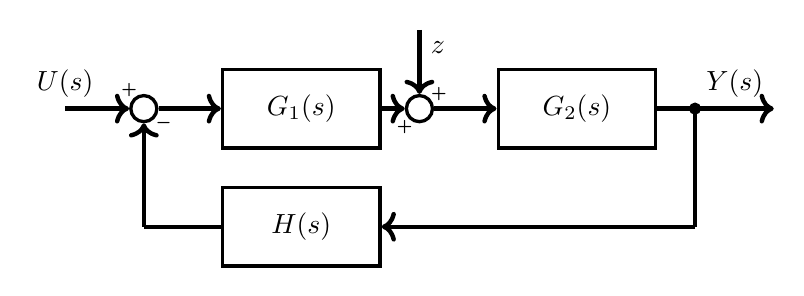
\begin{tikzpicture}[scale=2]
    \node[sum](sum)at(-1,0){};
    \node[sum](sum2)at(0.75,0){};
    \draw[->,ultra thick](-1.5,0)node[above]{$U(s)$}--(sum.180)node[above]{$\scriptscriptstyle\boldsymbol{+}$};


    \node[block, right of=sum, node distance=2cm](g){$G_1(s)$};
    \draw[->,ultra thick](sum.0)--(g.180);
    \draw[->,ultra thick](g.0)--(sum2.180)node[below]{$\scriptscriptstyle\boldsymbol{+}$};
    

    \filldraw[black](2.5,0)circle(1pt);


    \draw[->,ultra thick](0.75,0.5)node[below right]{$z$}--(sum2.90)node[right]{$\scriptscriptstyle\boldsymbol{+}$};

    \node[block]at(1.75,0)(k){$G_2(s)$};
    \draw[->,ultra thick](sum2.0)--(k.180);
    \draw[-,ultra thick](k.0)--(2.5,0);

    \draw[->,ultra thick](2.5,0)node[above right]{$Y(s)$}--(3,0);
    \draw[-,ultra thick](2.5,-0.75)--(2.5,0);

    %\node[sum](sum3)at(1.75,-0.75){};
    %\draw[->,ultra thick](2.5,-0.75)--(sum3.0)node[above]{$\scriptscriptstyle\boldsymbol{+}$};
    %\draw[->,ultra thick](1.75,-1.25)node[right]{$h$}--(sum3.270)node[left]{$\scriptscriptstyle\boldsymbol{+}$};


    \node[block, below of=g, node distance=1.5cm](h){$H(s)$};
    %\draw[->,ultra thick](sum3.180)--(h.0);
    \draw[->,ultra thick](2.5,-0.75)--(h.0);
    \draw[-,ultra thick](h.180)--(-1,-0.75);

    \draw[->,ultra thick](-1,-0.75)--(sum.270)node[right]{$\scriptscriptstyle\boldsymbol{-}$};
\end{tikzpicture}\end{center}

A ciclo aperto il rumore ha un effetto sull'uscita $y_{z,F}=G_2z$, a ciclo chiuso ha un effetto $y_{z,W}=\displaystyle\frac{G_2z}{1+F}$. Il rumore ha un fattore di riduzione 
$1+F$, per determinare l'effetto del rumore sul ciclo chiuso si considera $\displaystyle\frac{y_{z,W}}{y_{z,F}}$. Si considera l'errore massimo causato dal rumore in quell'
intervallo di frequenze $K$, per poter filtrare il rumore in quell'intervallo di frequenze bisogna che il suo effetto sul ciclo chiuso sia minore di questo errore:
$\left|\displaystyle\frac{y_{z,W}}{y_{z,F}}\right|=\frac{1}{|1+F|}<\frac{1}{K}\Rightarrow|1+F|>K$. Per poter rigettare l'errore la funzione a ciclo aperto deve avere 
modulo maggiore di $K$ nell'intervallo di frequenze su cui agisce l'errore. In caso sia presente un errore di aliasing, allora bisongerà avere un modulo minore di un 
certo valore, in un intervallo di frequenze. \\

Questi tipi di errori vengon rappresentati nel diagramma di Bode del modulo come una finestra o rettangolo di base l'intervallo di frequenza nel cui sono presenti, e di 
altezza il modulo che la funzione deve supereare per evitare l'errore. Quando si usano reti correttrici per traslare la pulsazione di taglio bisogna considerare se la 
funzione intersechi completamente o in parte questa finestra, in caso bisona diminuire le aspettative del sistema e scegliere speciche che permettano la stabilità in quella 
situazione. 

\subsection{Teoria di Lyapunov}

Lyapunov alle fine dell'$800$ descrisse i sistemi non lineari ed un criterio sulla loro stabilità. \\

Per un sistema lineare autonomo $\dot x=f(x)$, si può considerare come un 
sistema a controreazione con un controllore che ne calcola l'entrata per cui non ha bisogno di un entrata esterna. Il sistema è in uno stato di equilibrio per 
$\dot x=0\Rightarrow f(x)=0$, può presentare un numero infinito di punti di equilibrio. Se per un valore di $\varepsilon$ arbitrariamente piccolo, raggio di un intorno 
circolare di un punto di equilirbio del sistema, esiste un intorno circolare di raggio $\delta_{\varepsilon}$ che contiene l'effetto del sistema, il sistema ha un'evoluzione 
limitata. Un sistema si dice quindi semplicemente stabile se:

\begin{equation}
    \exists\varepsilon>0\mbox{ t.c. }||x-x_{eq}||<\varepsilon\Rightarrow||x(t)-x_{eq}||<\delta_{\varepsilon}
\end{equation}

Per ogni intorno $\delta_{\varepsilon}$ del punto di equilibrio deve esistere un punto tale che la sua evoluzione rimanga contenuta in quel intorno circolare. 
Se $\lim_{t\to+\infty}x(t)=x_{eq}$ il sistema si dice asintoticamente stabile. \\

Poiché i sistemi linearei convergono esponenzialmente, se un sistema non lineare converge più velocemente di un qualsiasi esponenziale, si dice stabile esponenzialmente. 
Un sistema non lineare è stabile se esiste un intorno di stabilità, dove ogni evoluzione del sistema è almeno semplicemente stabile. Se esiste un unico punto di equilibrio del 
sistema è possibile che l'intorno sia infinto. \\

Sia $V(x)$ la funzione di stato del sistema, positiva per ogni valore di $x$, questa funzione avrà un valore vicino allo zero solo 
nell'intorno del punto di equilibrio, minimo della funzione. Si rappresenta con delle curve di livello, curve dove il valore di $V(x)$ è costante fino al valore 
$V(x_{eq})$, se il sistema è stabile nel punto $X_{eq}$ allora le curve di livello tenderanno a restringersi intorno a quel punto. \\

Se la derivata della funzione di stato, in ogni punto del sistema, è defintia e negativa, allora il sistema è asintoticamente stabile, per ogni stato del sistema $V$ la sua 
evoluzione non potrà che diminuire.

\begin{equation}
    \dot V(x)=\displaystyle\frac{dV}{dx}\frac{dx}{dt}=\frac{dV}{dx}f(x)<0,\:\forall x
\end{equation}

Questa funzione di stato viene chiamata funzione di Lyapunov, dopo aver determinato la funzione di Lyapunov di un sistema non lineare si può controllare la sua stabilità. 
Il teorema di LaSalle afferma che lo stato di un sistema non lineare tende asintoticamente al valore del suo invariante massimo, dove l'invariante massimo $M$ è un sottoinsieme 
dell'insieme $E$ dei punti per cui la derivata della funzione di Lyapunov si annulla: $M\subset E:=\{x\in I_{\delta_{\varepsilon}}(x_{eq})\big|\dot V(x)=0\}$. \\

Un sistema non lineare si può linearizzare intorno ad un suo punto di equilibrio, con $\Delta x=x-x_{eq}$, considerando l'espansione di Taylor della funzione $f(x)$ che 
definisce il sistema:

\begin{gather}
    f(x)=\cancelto{0}{f(x_{eq})}+\displaystyle\frac{f'(x_{eq})}{1!}{(x-x_e)}+...\\
    f(x)\approx f'(x_{eq})\Delta x\\
    \begin{cases}
        \dot x=f(x)\\
        f(x_{eq})=0
    \end{cases}\\
    \begin{cases}
        \Delta\dot x=f(x)\\
        f(x_{eq})=f'(x_{eq})\Delta x
    \end{cases}\\
    \Delta\dot x=f'(x_{eq})\Delta x
\end{gather}

Considerando un sistema non lineare con un entrata $u(t)$, definito da $\dot x=f(x,u)$, si può linearizzare considerando: 

\begin{equation}
    \Delta\dot x=\displaystyle\frac{\partial f}{\partial x}\bigg|_{x_{eq}}\Delta x+\frac{\partial f}{\partial u}\bigg|_{u_{eq}}\Delta u=\left(\mathbf{J}f\bigg|_{(x_{eq},u_{eq})}\cdot
    \begin{bmatrix}
        \Delta x\\
        \Delta u
    \end{bmatrix}
    \right)
\end{equation}

Dove $\mathbf{J}f$ è il Jacobiano della funzione $f$. \\

Se il sistema $\sum_L$ linearizzato è asintoticamente stabile allora anche il sistema non lineare $\sum_{NL}$ è asintoticamente stabile, se $\sum_L$ è instabile lo è 
anche $\sum_{NL}$, se $\sum_L$ è al limite di stabiltià, non si può stabilire il comportamento di $\sum_{NL}$. Per cui il sistema $\sum_{NL}$ si può stabilizzare 
localmente, agendo sul sistema linearizzato $\sum_L$. Per controllare l'intorno di stabilità, si simula l'evoluzione del sistema. 

\begin{center}\begin{tikzpicture}[scale=2]
    \coordinate(sum)at(-1,0){};
    \draw[->,ultra thick](-1,0)node[above right]{$u$}--(c.180);
    \node[block, right of=sum, node distance=2cm](c){$f(x,u)$};

    %\draw[->,ultra thick](sum.0)--(c.180);
    \filldraw[black](2.5,0)circle(1pt);

    \draw[->,ultra thick](2.5,0)node[above right]{$x$}--(3,0);
    \draw[-,ultra thick](2.5,-0.75)--(2.5,0);

    %\node[block]at(0.75,-0.75)(h){$H(s)$};
    \node[block]at(1.75,0)(p){$\displaystyle\frac{1}{s}$};

    \draw[-,ultra thick](p.0)--(2.5,0);
    \draw[->,ultra thick](c.0)node[above right]{$\dot x$}--(p.180);

    %\draw[->,ultra thick](2.5,-0.75)--(h.0);
    %\draw[-,ultra thick](h.180)--(-1,-0.75);
    \draw[-,ultra thick](2.5,-0.75)--(0,-0.75);
    \draw[->,ultra thick](0,-0.75)--(c.270);
\end{tikzpicture}\end{center}

\clearpage

\section{Sistemi a Segnali Campionati}

All'inizio del $900$ vennero usati sistemi di controllo anaogici, nel tempo questi componenti analogici sono stati sostituiti da componenti digitali. Per cui sistemi elettronici 
come gli amplificatori sono stati sostituiti da oggetti informatici, ovvero microprocessori insieme ad altri elementi. Usando componenti digitali è possibile programmare 
controllori schedulati, in grado di avere più di un algoritmo di controllo adatti per diversi stati del processo.    

\subsection{Microcontrollore}

Un microcontrollore è un oggetto fisico input-output capace di dialogare con l'ambiente esterno, all'interno di un chip, anche molto economico. Sono oggetti che presentano 
all'interno un microprocessore, quindi sono in grado di risolvere piccoli problemi di automazione. Dei PLC sono invece dei controllori più sofisticati che permettono di 
avere frequenze di aggiornamento molto elevate e trasmissione di dati costante. 
\\
Un microcontrollore è composto da un microprocessore $\mu P$, convertitori da digitale ad analogico $DAC$, per poter dialogare con un certo processo $P$ da controllare, 
convertendo i dati del processo in livelli di tensione. Poiché il microprocessore digatale lavora in bit, mentre il processo analogico da controllare è continuo, sarà 
necessario convertire questi dati. La tensione in uscita dal $DAC$ è di bassa potenza, per cui è presenta a cascata un amplificatore $A$ alimentato da un 
generatore di tensione esterno $V_{cc}$, per avere in uscita livelli di tensione adeguati. 
\\
Per pulire i segnali misurati si usa in catena di misura un filtro-antialiasing, il segnale viene poi passato ad un convertitore $ADC$ che lo trasforma in discreto. 
Il microprocessore informa il convertitore 
$ADC$ con un segnale $SOC$ per iniziare la conversione, il quale invia un segnale $EOC$ al microprocessore per segnalare la fine della conversione del dato. A quel punto 
il microprocessore leggerà sul bus il dato convertito. Si può inserire un circuito di adattamento $a$ tra il filtro antialiasing ed il convertitore $ADC$, per adattare 
l'uscita in tensione del processo all'ingresso in tensione dei convertitori. Poiché i convertitori hanno un certo intervallo di ingresso accettabile in Volt, il dato 
ottenuto operando su quello grezzo del sensore viene chiamato dato ingegnerizzato. 
\\
Il valore di riferimento $r$ del microcontrollore può essere computato o inserito da un segnale esterno. Il microcontrollore $\mu C$ comprende il microprocessore, ed i convertitori 
$DAC$ e $ADC$, anche su un singolo chip. I collegamenti tra i convertitori ed il microprocessore sono dei $BUS$ a $n$ bit, mentre il resto dei collegamenti sono 
segnali continui. 

\begin{center}
    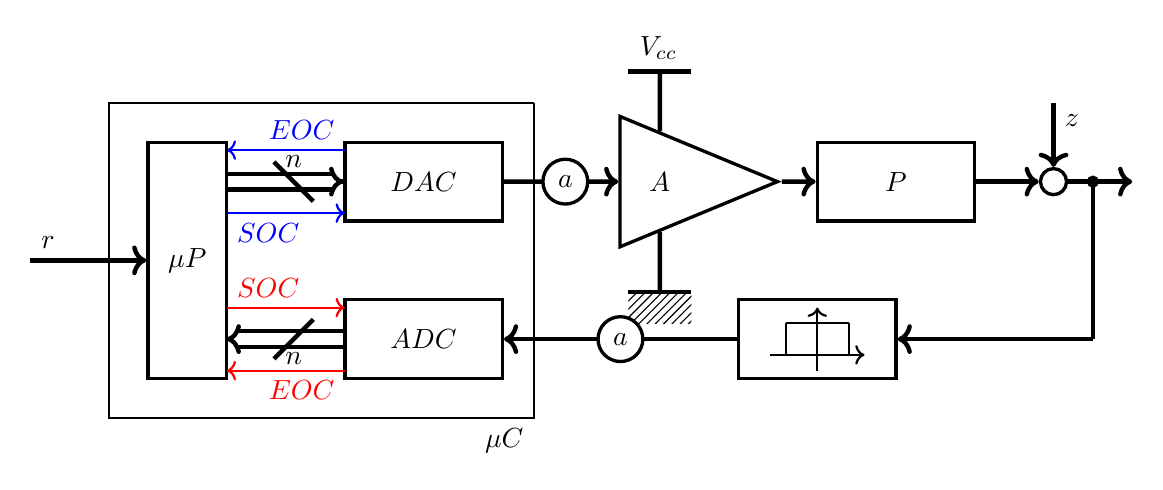
\begin{tikzpicture}[scale=2]
        \node[lblock](mp)at(-0.5,0){$\mu P$};
        \node[block](dac)at(1,0.5){$DAC$};
        \node[block](ad)at(1,-0.5){$ADC$};

        \draw[-,ultra thick](-0.25,0.45)--(0.42,0.45);
        \draw[-,ultra thick](-0.25,0.55)--(0.42,0.55);
        \draw[<-,ultra thick](0.49,0.5)--(dac.180);
        \draw[-, ultra thick](0.05,0.625)node[right]{$n$}--(0.3,0.375);
        %       (0.175,0.5)
        \draw[-,ultra thick](-0.17,-0.45)--(0.5,-0.45);
        \draw[-,ultra thick](-0.17,-0.55)--(0.5,-0.55);
        \draw[->,ultra thick](-0.24,-0.5)--(-0.25,-0.5);
        \draw[-, ultra thick](0.05,-0.625)node[right]{$n$}--(0.3,-0.375);

        \draw[<-,thick, blue](-0.25,0.7)--(0.5,0.7)node[above left]{$EOC$};
        \draw[->,thick, blue](-0.25,0.3)node[below right]{$SOC$}--(0.5,0.3);        
        \draw[->,thick, red](-0.25,-0.3)node[above right]{$SOC$}--(0.5,-0.3);        
        \draw[<-,thick, red](-0.25,-0.7)--(0.5,-0.7)node[below left]{$EOC$};


        \node[triangle](t)at(2.5,0.5){$A$};
        \draw[->,ultra thick](dac.0)--(t.180);
        \draw[-, ultra thick](2.5,1.2)--(t.90);
        \draw[-, ultra thick](2.3,1.2)node[above right]{$V_{cc}$}--(2.7,1.2);
        \draw[-, ultra thick](t.270)--(2.5,-0.2);
        \draw[-, ultra thick](2.3,-0.2)--(2.7,-0.2);
        \fill[pattern = north east lines]($ (2.3,-0.4) $)rectangle($ (2.7,-0.2)$);

        \node[block](p)at(4,0.5){$P$};
        \draw[->,ultra thick](t.0)--(p.180);
        \node[sum](z)at(5,0.5){};
        \draw[->,ultra thick](p.0)--(z.180);
        \draw[->, ultra thick](z.0)--(5.5,0.5);
        \draw[->, ultra thick](5,1)node[below right]{$z$}--(z.90);
        \filldraw[black](5.25,0.5)circle(1pt);


        \node[nblock](aa)at(3.5,-0.5){};
        \draw[->, thick](3.2,-0.6)--(3.8,-0.6);
        \draw[->, thick](3.5,-0.7)--(3.5,-0.3);
        \draw[-,thick](3.3,-0.4)--(3.7,-0.4);
        \draw[-,thick](3.3,-0.4)--(3.3,-0.6);
        \draw[-,thick](3.7,-0.4)--(3.7,-0.6);

        \draw[-,ultra thick](5.25,-0.5)--(5.25,0.5);
        \draw[->,ultra thick](5.25,-0.5)--(aa.0);
        \draw[->,ultra thick](aa.180)--(ad.0);
        \node[sum](ca1)at(2.25,-0.5){$a$};
        \node[sum](ca2)at(1.9,0.5){$a$};


        \draw[->,ultra thick](-1.5,0)node[above right]{$r$}--(mp.180);

        \draw[-,thick](1.7,1)--(1.7,-1)node[below left]{$\mu C$}--(-1,-1)--(-1,1)--(1.7,1);
    \end{tikzpicture}
\end{center}

\subsubsection{Quantizzazione}

Un dato digitale viene rappresentato da un certo numero $n$ di bit, per cui può rappresentare valori nell'intervallo $[0,2^n-1]$. Un convertitore $DAC$ suddivide l'intervallo 
di tensione in entrata in $2^n$ intervalli uguali e ogni valore che un bit può rappresentare corriponsderà quindi ad un intervallo di tensione. Non è possibile determinare 
in questo modo la tensione esatta, questo effetto viene chiamato quantizzazione, ed è quantificabile dal passo di quantizzazione, ovvero la grandezza di un singolo intervallo 
di tensione, o gradino:

\begin{equation}
    q=\displaystyle\frac{\Delta V}{2^n}
\end{equation}

\begin{center}
    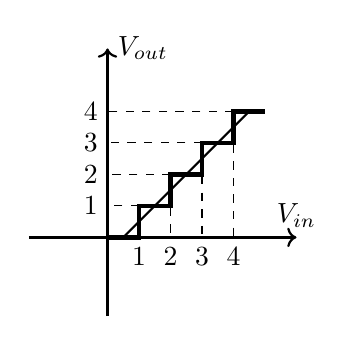
\begin{tikzpicture}[scale=2]
        \draw[->, thick](-0.5,0)--(1.2,0)node[above]{$V_{in}$};
        \draw[->, thick](0,-0.5)--(0,1.2)node[right]{$V_{out}$};

        \draw[thick](0.1,0)--(0.9,0.8);

        \draw[-, ultra thick](0,0)--(0.2,0)--(0.2,0.2)--(0.4,0.2)--(0.4,0.4)--(0.6,0.4)--(0.6,0.6)--(0.8,0.6)--(0.8,0.8)--(1,0.8);
        \draw[dashed](0.2,0.2)--(0.2,0)node[below]{$1$};
        \draw[dashed](0.4,0.4)--(0.4,0)node[below]{$2$};
        \draw[dashed](0.2,0.2)--(0,0.2)node[left]{$1$};
        \draw[dashed](0.4,0.4)--(0,0.4)node[left]{$2$};
        \draw[dashed](0.6,0.6)--(0,0.6)node[left]{$3$};
        \draw[dashed](0.6,0.6)--(0.6,0)node[below]{$3$};
        \draw[dashed](0.8,0.8)--(0,0.8)node[left]{$4$};
        \draw[dashed](0.8,0.8)--(0.8,0)node[below]{$4$};
    \end{tikzpicture}
\end{center}
Per cui è impossibile determinare a meno del passo di quantizzazione una certa uscita, e quindi il controllore avrà un errore minimo uguale al passo di quantizzazione, 
poiché non può agire su ciò che non può misurare. \`{E} necessario decidere a priori il passo di quantizzazione necessario per l'applicazione del controllore. 
Poiché la quantizzazione è un processo non lineare, si considerererà sempre nelle successive analisi come se si fosse scelto il numero di bit sufficiente per le applicazioni 
considerate. Verrà considerato alla fine un rumore di quantizzazione dovuto alla differenza tra la suddivisione in gradini e l'andamento lineare. 

Per scegliere il numero di bit adatto, si analizza l'oscillazione del segnale e si misura la varianza rispetto al valor medio e si calcola il valore di rumore in percentuale 
$z[\%]$, e si sceglie un numero di bit abbastanza piccolo da non campionare il rumore $n\mbox{ t.c. }\displaystyle\frac{1}{n}>\frac{z}{100}$, poiché essendo casuale il 
controllore non potrà agire su di esso. 

Se si scelgono troppi pochi bit, il segnale potrebbe variare senza una variazione nella sua rappresentazione. 

In genere i convertitori $ADC$ possono convertire valori di tensioni di queste tipologie: $[0,5]$, $[0,10]$, $[-5,+5]$, $[-10,+10]$, $[0,20]$. Alcuni convertitori, convertoto 
correnti invece di tensioni. Per adeguare le tensioni delle varie componenti del sistema, vengono usati circuiti di adattamento tra i convertitori in entrata ed in uscita del 
microcontrollore che applicano le opportune traslazioni e amplificazioni del segnale. 

Poiché un processore non può convertire costantemente il segnale, sono necessari dei segnali di controllo per iniziare e terminare la conversione. Questi segnali sono $SOC$ e 
$EOC$, $Start\:Of\:Conversion$ e $End\:Of\:Conversion$, sia per $ADC$ che per il $DAC$. Quindi solo grazie a questi segnali è possibile portare il dato dentro e fuori il 
microcontrollore in sicurezza, realizzati tramite degli $interrupt$.  

\subsubsection{Tempo di Campionamento}

Il microprocessore invia il segnale $SOC$ al convertitore $ADC$. Il convertitore effettua un $hold$ del segnale in entrata e comincia a campionarlo, alla fine del campionamento  
invia i dati nel $BUS$ ed invia il segnale $EOC$ al microprocessore. A questo punto il processore legge i dati dal $BUS$ e li elabora, $signal\:\:processing$ in un tempo 
relativamente più o meno lungo, al termine il calcolato su un registro interno del processore viene inviato al convertitore $DAC$ con un segnale $SOC$. Il $DAC$ converte il 
segnale in continuo ed al termine della conversione invia un segnale $EOC$ al microprocessore. 

\begin{center}
    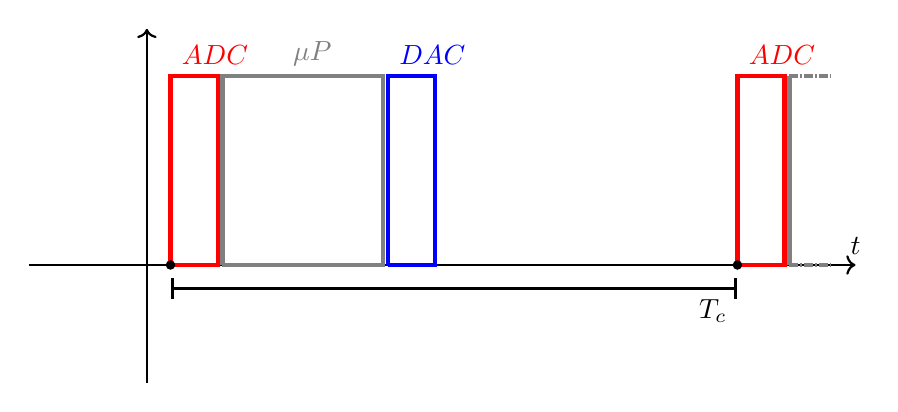
\begin{tikzpicture}[scale=3]
        \draw[->, thick](-0.5,0)--(3,0)node[above]{$t$};
        \draw[->, thick](0,-0.5)--(0,1);

        \draw[-,ultra thick, red](0.1,0)--(0.1,0.8)node[above right]{$ADC$}--(0.3,0.8)--(0.3,0)--(0.1,0);
        \draw[-,ultra thick, gray](0.32,0)--(0.32,0.8)--(1,0.8)--(1,0)--(0.32,0);
        \node[gray, above]at(0.7,0.8){$\mu P$};
        \draw[-,ultra thick, blue](1.02,0)--(1.02,0.8)node[above right]{$DAC$}--(1.22,0.8)--(1.22,0)--(1.02,0);

        \filldraw[black](0.1,0)circle(0.5pt);
        \draw[-,ultra thick, red](2.5,0)--(2.5,0.8)node[above right]{$ADC$}--(2.7,0.8)--(2.7,0)--(2.5,0);
        \draw[-,ultra thick, gray](2.72,0)--(2.72,0.8);
        \draw[densely dashdotted,ultra thick, gray](2.72,0)--(2.9,0);
        \draw[densely dashdotted,ultra thick, gray](2.72,0.8)--(2.9,0.8);       
        \filldraw[black](2.5,0)circle(0.5pt);

        \draw[|-|,very thick](0.1,-0.1)--(2.5,-0.1)node[below left]{$T_c$};
    \end{tikzpicture}
\end{center}

Il microprocessore dopo questo tempo potrebbe fare housekeeping, operazioni interne non relative alla conversione, e ricomincia a convertire i dati dopo un intervallo di tempo. 
Questo intervallo di tempo viene chiamato tempo di campionamento $T_c$, comprende il tempo necessario per il microcontrollore di convertire ed elaborare i dati, ed il tempo 
delle operazioni di housekeeping. Questo tempo di campionamento è intrinseco al microcontrollore e non è variabile, per cui alcuni microcontrollori sono poco utili per 
un tempo di campionamento troppo grande. Può essere presente jitter che cambia l'andmaento del processo collegato al controllore. La scelta di un microcontrollore dipenderà 
quindi dal tempo di campionamento necessario per controllare un dato processo. 

Per comunicare al microprocessore l'inizio e la fine della conversione vengono usati degli $interrupt$, segnali che avvertono il processore che è successo qualcosa. Ogni 
volta che è necessario compiere delle azioni periodiche, bisogna associare dei segnali di $interrupt$ a segnali esterni, dei $clock$, oppure da un programma interno. Il 
programma di controllo definito viene gestito dal sistema operativo. Esistono vari tipi di interrupt mascherabili e non, alcuni si possono disabilitare. In caso un programma 
sia in idle da molto tempo viene spostato dalla $RAM$ per liberare spazio agli interrupt che arrivano al microprocessore in quel tempo. Il sistema operativo standard ha un 
tempo di campionamento di $1\:s$ ed un jitter di circa $1:ms$, per cui è difficile avere un tempo di campionamento minore di un $ms$ suu un SO genral purpose. Per questo 
delle task time critical necessitano di sistemi operativi dedicati ai controllori, dato che alcuni sistemi operativi pre-emptive hanno delle ruotine programmate per essere 
interrote da alcune operazini del kernel. Di conseguenza alcune operazioni che sembrano real-time avvengono in intervalli precisi per farle sembrare real-time. 
Si definisce allora una ruotine soft real time, per processi che si aggiornano solo ogni $n\:\:ms$ con un margine di errore elevato, mentre si definisce una ruotine hard real 
time se il mancato rispetto di una task diviene risulta in danni gravi per l'infrastruttura su cui opera. 

Per analizzare questo processo bisogna definire un sistema per descrivere oggetti continui nel discreto, tempi multipli del tempo di campionamento, tramite il teorema del 
campionamento. Viene inoltre definita la trasformata $z$ per studiare elementi totalmente discreti, trasformata omologa a quella di Laplace. 

\subsection{Rappresentazione Segnali Campionati}

Dato lo stato nel tempo di un sistema $x(t)$, se si implementa un controllore digitale, si avrà accesso solo ad una sequenza di stati $\{x_k\}$ dove ogni stato è dato dallo 
stato del sistema in un tempo multiplo del tempo di campionamento $x_k=x(kT_c)$. In questo modo si ha una sequenza di valori, campionati dal convertitore $ADC$ ogni $T_c$. Se 
consideriamo una serie di impulsi ogni tempo di campionamento di ampiezza il valore campionato in quel'istante, si può approssimare la funzione continua sulla base dei 
valori discreti. Per ottenere la funzione originaria servirebbe un tempo di campionamento tendende a zero. Il segnale campionato sarà dato 
dalla sommatoria di impulsi traslati di un multiplo del tempo di campionamento:

\begin{equation}
    x_c(t)=\sum_{k=0}^{\infty}x_k\delta_0(t-kT_c)
\end{equation}

\begin{center}
    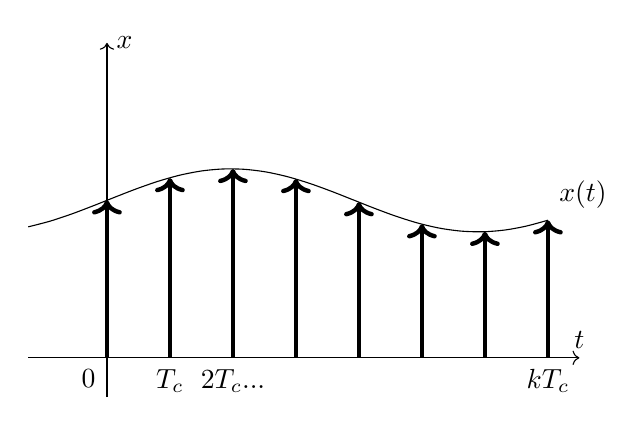
\begin{tikzpicture}[scale=2]
        \draw[->](0,-0.25)--(0,2)node[right]{$x$};
        \draw[->](-0.5,0)--(3,0)node[above]{$t$};

        \draw[]plot[smooth, domain=-0.5:2.8](\x,{1+0.2*sin(2*\x r)});
        \draw[->,ultra thick](0,0)node[below left]{$0$}--(0,1);
        \draw[->,ultra thick](0.4,0)node[below]{$T_c$}--(0.4,1.141);
        \draw[->,ultra thick](0.8,0)node[below]{$2T_c...$}--(0.8,1.199);
        \draw[->,ultra thick](1.2,0)--(1.2,1.135);
        \draw[->,ultra thick](1.6,0)--(1.6,0.988);
        \draw[->,ultra thick](2,0)--(2,0.848);
        \draw[->,ultra thick](2.4,0)--(2.4,0.8);
        \draw[->,ultra thick](2.8,0)node[below]{$kT_c$}--(2.8,0.873)node[above right]{$x(t)$};
    \end{tikzpicture}
\end{center}

La sequenza di impulsi ha esattamente il contenuto informativo della sequenza di valori misurati $\{x_k\}$, poiché l'impulso ha un'area infinitesima. Per cui è possibile 
usarlo per lavorare sul tempo discreto. Da un qualsiasi segnale campionato è quidni possibile ottenere la sua trasformata di Laplace:

\begin{equation}
    x_c(s)=\sum_{k=0}^{\infty}\displaystyle{x_k}e^{-skT_c}
\end{equation}

Per cui ha una sua risposta in frequenza, e probabilmente un suo diagramma di Bode. Considerando $s=\sigma +j\omega$, si può riscrivere come: 

\begin{equation}
    x_c(s)=\sum_{k=0}^{\infty}x_ke^{-\sigma kT_c}e^{-j\omega kT_c}
\end{equation}

Data una pulsazione di campionamento $\omega_c=2\pi\nu_c=\displaystyle\frac{2\pi}{T_c}$, si potrà riscrivere la parte complessa dell'esponenziale come:

\begin{equation}
    e^{-j\omega kT_c}=e^{-2j\pi k\frac{\omega}{\omega_c}}
\end{equation}

Questo oggetto sarà periodico nell'intervallo $\left[\displaystyle-j\frac{\omega_c}{2},j\frac{\omega_c}{2}\right]$, poiché per $\omega'=\omega_c+\omega$ si ha 
$-2j\pi k\displaystyle\frac{\omega'}{\omega_c}=-2j\pi k\left(1+\frac{\omega}{\omega_c}\right)=-2j\pi k-2j\pi k\frac{\omega}{\omega_c}$, quindi l'esponenziale sarà: 
$e^{-2j\pi k\frac{\omega'}{\omega_c}}=\cancelto{1}{e^{-2j\pi k}}\cdot e^{-2j\pi k\frac{\omega}{\omega_c}}$. Dipendendo dalla sola componente immaginaria, sarà 
periodico per ogni valore complesso avente parte immaginaria compresa in quell'intervallo. Il piano di Gauss sarà quindi diviso in strisce uguali di ampiezza $\omega_c$. 
Per cui la trasformata di Laplace di un segnale reale periodico sarà anch'essa periodica, si studierà quindi un'unica di queste strisce. 

\begin{center}
    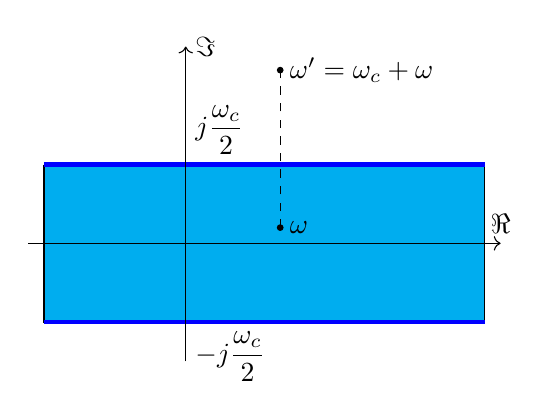
\begin{tikzpicture}[scale=2]
        \draw[fill=cyan](-0.9,0.5)--(1.9,0.5)--(1.9,-0.5)--(-0.9,-0.5)--(-0.9,0.5);
        \draw[-, blue,ultra thick](-0.9,0.5)--(1.9,0.5);       
        \draw[-, blue,ultra thick](-0.9,-0.5)--(1.9,-0.5);

        \draw[->](-1,0)--(2,0)node[above]{$\Re$};
        \draw[->](0,-0.75)--(0,1.25)node[right]{$\Im$};

        \node[above right]at(0,0.5){$\displaystyle j\frac{\omega_c}{2}$};
        \node[below right]at(0,-0.5){$\displaystyle -j\frac{\omega_c}{2}$};

        \filldraw[black](0.6,0.1)node[right]{$\omega$}circle(0.5pt);
        \filldraw[black](0.6,1.1)node[right]{$\omega'=\omega_c+\omega$}circle(0.5pt);
        \draw[dashed](0.6,0.1)--(0.6,1.1);
    \end{tikzpicture}
\end{center}

\subsubsection{Teorema del Campionamento}

Si definisce un nuovo segnale $\delta_R(t)$, formato da una rastregliera di impulsi unitari ogni $T_c$:
\begin{equation}
    \delta_R(t)=\sum_{k=0}^{\infty}\delta_0(t-kT_c)
\end{equation} 
\begin{center}
    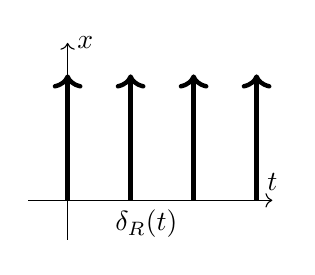
\begin{tikzpicture}[scale=2]
        \draw[->](-0.25,0)--(1.3,0)node[above]{$t$};
        \draw[->](0,-0.25)--(0,1)node[right]{$x$};
        \draw[->,ultra thick](0,0)--(0,0.8);
        \draw[->,ultra thick](0.4,0)--(0.4,0.8);
        \draw[->,ultra thick](0.8,0)--(0.8,0.8);
        \draw[->,ultra thick](1.2,0)--(1.2,0.8);
        
        \node[below]at(0.5,0){$\delta_R(t)$};
    \end{tikzpicture}
\end{center}
Moltiplicando la rastregliera con il segnale da campionare $x(t)$, si ottiene il segnale campionato. Da tenere conto del fatto che una rastregliera non è una funzione, 
essendo discreta, mentre il segnale da campionare essendo nel continuo è una funzione. 
\begin{equation}
    x_c(t)=x(t)\cdot\delta_R(t)
\end{equation}
\begin{center}
    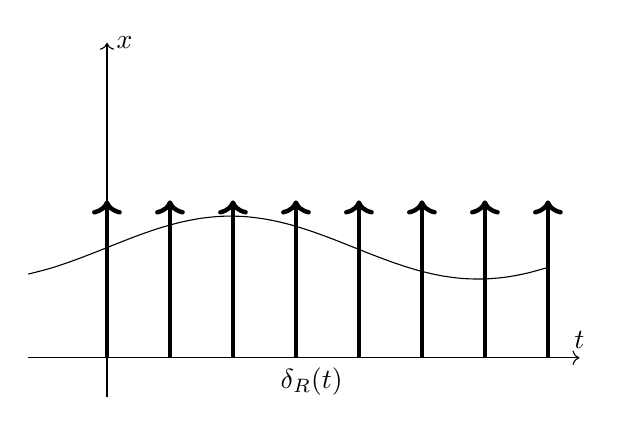
\begin{tikzpicture}[scale=2]
        \draw[->](0,-0.25)--(0,2)node[right]{$x$};
        \draw[->](-0.5,0)--(3,0)node[above]{$t$};

        \draw[]plot[smooth, domain=-0.5:2.8](\x,{0.7+0.2*sin(2*\x r)});

        \draw[->,ultra thick](0,0)--(0,1);
        \draw[->,ultra thick](0.4,0)--(0.4,1);
        \draw[->,ultra thick](0.8,0)--(0.8,1);
        \draw[->,ultra thick](1.2,0)--(1.2,1);
        \draw[->,ultra thick](1.6,0)--(1.6,1);
        \draw[->,ultra thick](2,0)--(2,1);
        \draw[->,ultra thick](2.4,0)--(2.4,1);
        \draw[->,ultra thick](2.8,0)--(2.8,1);

        \node[below]at(1.3,0){$\delta_R(t)$};

    \end{tikzpicture}
\end{center}
Nei punti di intersezione tra gli impulsi della rastregliera ed il segnale $x(t)$ verrà campionata l'ampiezza. 

La funzione rastregliera è periodica, dall'analisi di Fuorier, ogni funzione periodica può essere scritta come una sommatoria di funzioni sinusoidali e consenusoidali, per 
cui si considera la funzione rastregliera come:
\begin{equation}
    \delta_R(t)=c_0+\sum_{k=0}^{\infty}\left(a_ksin(k\omega_ct)+b_kcos(k\omega_ct)\right)
\end{equation}
Può essere espressa tramite la rappresetnazione di Eulero in forma esponenziale:
\begin{equation}
    \delta_R(t)=\sum_{k=-\infty}^{\infty}c_ke^{jk\omega_ct}
\end{equation}
Dati un seno ed un coseno aventi coefficienti $a_k$ e $b_k$, la loro somma sarà data da un seno ed un coseno moltiplicati da uno stesso coefficiente ed un certo sfasamento. 
Per ottenere questo coefficiente bisogna ottenere le compomnenti della serie di Fuorier rispetto ad un sistema di coordinate ortogonali. La trasformata di Fuorier è un elemento basilare per analizzare 
i segnali, trasportandoli dal dominio del tempo nel dominio dellla frequenza. Per ottenere la 
proiezione di un vettore $\vec{v}=v_k\hat{k}+v_j\hat{j}$ rispetto ad una coordinata $k$, si considera il prodotto scalare tra il vettore ed il versore della coordinata, 
per cui si avrà $v_k=\vec{v}\cdot\hat{k}$. 

Analogamente ad un prodotto scalare in uno spazio vettoriale, l'integrale di Fuorier agisce come un'operazione di proiezione. Per cui per trovare le componenti della rastregliera 
rispetto alla funzione $e^{jk\omega_ct}$ si considera l'integrale di Fuorier, a meno di un fattore di amplificazione: 
\begin{equation}
    c_k=\displaystyle\frac{1}{T_c}\int_{-\frac{T_c}{2}}^{\frac{T_c}{2}}\delta_R(t)e^{-jk\omega_ct}dt
\end{equation}

%L'integrale soddisfa i requisiti per essere un prodotto interno. Questo applicazione funziona fino a quando le funzioni sono indipendenti tra di loro, per determinare 
%se sono ortogonali tra di loro, si controlla che il prodotto interno tra due funzioni di base $f(t)=e^{jk\omega_ct}$ e $\varphi(t)=e^{jl\omega_ct}$ per $l\neq k$ sia zero:
%\begin{gather}
%    \displaystyle\frac{1}{T_c}\int_{-\frac{T_c}{2}}^{\frac{T_c}{2}}e^{jl\omega_ct}e^{-jk\omega_ct}dt=
%    \frac{1}{T_c}\left[\frac{e^{j(l-k)\omega_ct}}{j(l-k)\omega_c}\right]^{\frac{T_c}{2}=\frac{\pi}{\omega_c}}_{-\frac{T_c}{2}=-\frac{\pi}{\omega_c}}\\
%    \displaystyle\frac{1}{T_c}\frac{e^{j(l-k)\pi t}-e^{-j(l-k)\pi t}}{j(l-k)\omega_c}=\frac{2}{T_c(l-k)\omega_c}sin((l-k)\pi t)=0
%\end{gather} 
%Si è verificato che il prodotto interno definito precedentemente tra due funzioni di base è zero per $l\neq k$.

L'unico impulso della rastregliera che cade in quell'intervallo è nell'istante $t=0$. L'integrale di un prodotto tra una funzione e l'impulso, equivale a calocolare il valore 
della funzione in quel punto, per cui si ha:
\begin{equation}
    c_k=\displaystyle\frac{1}{T_c}e^{-jk\omega_c \cdot0}=\frac{1}{T_c}
\end{equation}

Per cui si può scrivere la rastregliera come:
\begin{equation}
    \delta_R(t)=\displaystyle\frac{1}{T_c}\sum_{k=-\infty}^{\infty}e^{jk\omega_ct}
\end{equation}
Il segnale campionato sarà allora:
\begin{gather}
    x_c(t)=x(t)\delta_R(t)=\displaystyle\frac{1}{T_c}\sum_{k=-\infty}^{\infty}x(t)e^{jk\omega_ct}\\
    X_c(s)=\mathscr{L}_-\{x_c(t)\}=\displaystyle\frac{1}{T_c}\sum_{k=-\infty}^{\infty}\mathscr{L}_-\left\{x(t)e^{jk\omega_ct}\right\}=\frac{1}{T_c}\sum_{k=-\infty}^{\infty}X(s-jk\omega_c)
\end{gather}
Per cui il segnale campionato in frequenza non è altro che una sommatoria del segnale originario traslato di una certa quantità, ovvero il teorema di Shannon scritto in 
Laplace. 

\subsubsection{Ricostruzione}

Per ritornare al teorema di Shannon, si considera solamente la sua rispsosta armonica, $s=j\omega$:
\begin{equation}
    X_c(j\omega)=\displaystyle\frac{1}{T_c}\sum_{k=-\infty}^{\infty}X(j(\omega-k\omega_c))
\end{equation}

Per cui l'oggetto che si ripete in frequenza si è scoperto essere la trasformata di Laplace del 
segnale originario. Rappresentando le frequenze su un asse delle ascisse e il modulo della risposta armonica sulle ordinate, si può rappresentare la trasformata di Fuorier 
come un diagramma di Bode. Rappresentando il diagramma di Bode del segnale originario in frequenza, ci sarà una singola curva, chiamata lobo, simmetrica rispetto all'asse 
delle ordinate, strettamente decrescente, se si considerando solo frequenze positive o negative. 
\begin{center}
    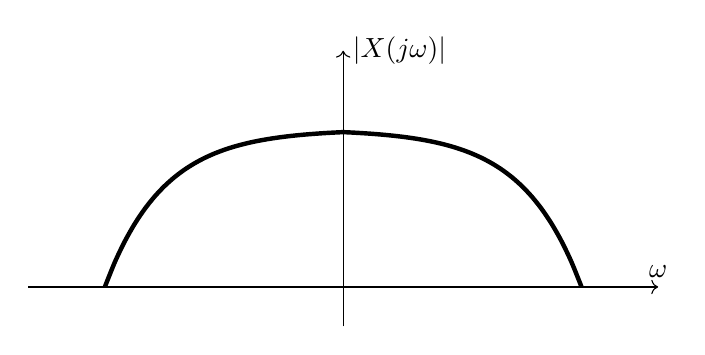
\begin{tikzpicture}[scale=2]
        \draw[->](-2,0)--(2,0)node[above]{$\omega$};
        \draw[->](0,-0.25)--(0,1.5)node[right]{$|X(j\omega)|$};

        \draw[ultra thick]plot[smooth, domain=0:1.513](\x,{1-0.25*e^(2.7*(\x-1))});
        \draw[ultra thick]plot[smooth, domain=-1.513:0](\x,{1-0.25*e^(-2.7*(\x+1))});

    \end{tikzpicture}
\end{center}

Poiché il segnale campionato in frequenza è una sommatoria delle trasformate di Laplace del segnale originale, traslate di $k\omega_c$, e ridotte di un fattore 
$\displaystyle\frac{1}{T_c}$, il suo diagramma di Bode sarà formato da una serie di lobi uguali ripetuti. 
\begin{center}
    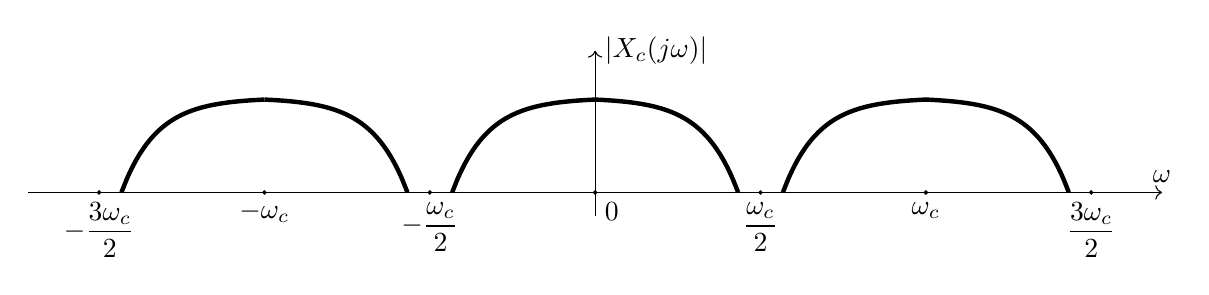
\begin{tikzpicture}[scale=1.2]
        \draw[->](-6,0)--(6,0)node[above]{$\omega$};
        \draw[->](0,-0.25)--(0,1.5)node[right]{$|X_c(j\omega)|$};

        \draw[ultra thick]plot[smooth, domain=0:1.513](\x,{1-0.25*e^(2.7*(\x-1))});
        \draw[ultra thick]plot[smooth, domain=-1.513:0](\x,{1-0.25*e^(-2.7*(\x+1))});

        \draw[ultra thick]plot[smooth, domain=-3.5:-1.987](\x,{1-0.25*e^(2.7*(\x+2.5))});
        \draw[ultra thick]plot[smooth, domain=-5.013:-3.5](\x,{1-0.25*e^(-2.7*(\x+4.5))});

        \draw[ultra thick]plot[smooth, domain=3.5:5.013](\x,{1-0.25*e^(2.7*(\x-4.5))});
        \draw[ultra thick]plot[smooth, domain=1.987:3.5](\x,{1-0.25*e^(-2.7*(\x-2.5))});

        \filldraw[black](1.75,0)node[below]{$\displaystyle\frac{\omega_c}{2}$}circle(0.5pt);
        \filldraw[black](-1.75,0)node[below]{$\displaystyle-\frac{\omega_c}{2}$}circle(0.5pt);
        \filldraw[black](3.5,0)node[below]{$\omega_c$}circle(0.5pt);
        \filldraw[black](-3.5,0)node[below]{$-\omega_c$}circle(0.5pt);
        \filldraw[black](5.25,0)node[below]{$\displaystyle\frac{3\omega_c}{2}$}circle(0.5pt);
        \filldraw[black](-5.25,0)node[below]{$\displaystyle-\frac{3\omega_c}{2}$}circle(0.5pt);
        \filldraw[black](0,0)node[below right]{$0$}circle(0.5pt);
  
    \end{tikzpicture}
\end{center}
In caso la metà della pulsazione di campionamento è maggiore della frequenza massima del segnale, allora i lobi 
saranno separati. Il segnale sarà multiplato in frequenza, uguale al segnale non campionato. Per cui si può usare un filtro passa basso fino a 
$\displaystyle\frac{\omega_c}{2}$, per isolare solamente il lobo centrale e amplificarlo di $T_c$ ottenendo il segnale originario. 
Questo segnale viene chiamato segnale ricostruito, è possibile in alcuni casi quindi ricostruire esattamente il segnale originario dati dei punti campionati. 

\begin{center}
    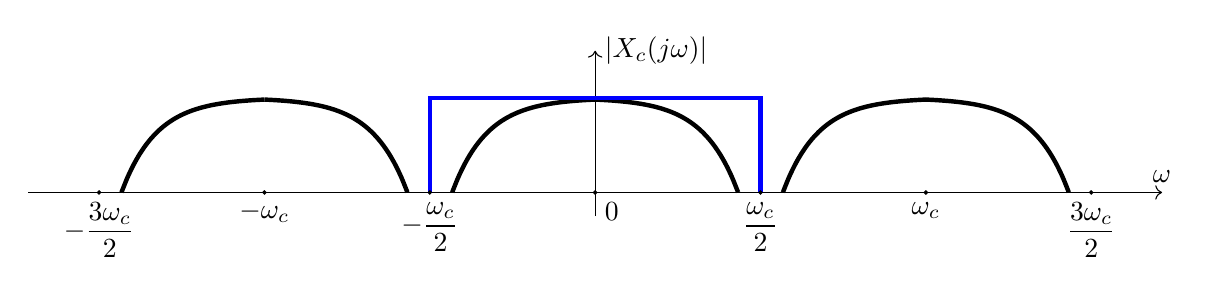
\begin{tikzpicture}[scale=1.2]
        \draw[->](-6,0)--(6,0)node[above]{$\omega$};
        \draw[->](0,-0.25)--(0,1.5)node[right]{$|X_c(j\omega)|$};

        \draw[ultra thick]plot[smooth, domain=0:1.513](\x,{1-0.25*e^(2.7*(\x-1))});
        \draw[ultra thick]plot[smooth, domain=-1.513:0](\x,{1-0.25*e^(-2.7*(\x+1))});

        \draw[ultra thick]plot[smooth, domain=-3.5:-1.987](\x,{1-0.25*e^(2.7*(\x+2.5))});
        \draw[ultra thick]plot[smooth, domain=-5.013:-3.5](\x,{1-0.25*e^(-2.7*(\x+4.5))});

        \draw[ultra thick]plot[smooth, domain=3.5:5.013](\x,{1-0.25*e^(2.7*(\x-4.5))});
        \draw[ultra thick]plot[smooth, domain=1.987:3.5](\x,{1-0.25*e^(-2.7*(\x-2.5))});

        \draw[-,ultra thick, blue](1.75,0)--(1.75,1)--(-1.75,1)--(-1.75,0);

        \filldraw[black](1.75,0)node[below]{$\displaystyle\frac{\omega_c}{2}$}circle(0.5pt);
        \filldraw[black](-1.75,0)node[below]{$\displaystyle-\frac{\omega_c}{2}$}circle(0.5pt);
        \filldraw[black](3.5,0)node[below]{$\omega_c$}circle(0.5pt);
        \filldraw[black](-3.5,0)node[below]{$-\omega_c$}circle(0.5pt);
        \filldraw[black](5.25,0)node[below]{$\displaystyle\frac{3\omega_c}{2}$}circle(0.5pt);
        \filldraw[black](-5.25,0)node[below]{$\displaystyle-\frac{3\omega_c}{2}$}circle(0.5pt);
        \filldraw[black](0,0)node[below right]{$0$}circle(0.5pt);
  

    \end{tikzpicture}
\end{center}

Shannon affermò che facendo passare un segnale per il filtro passa-basso mostrato in precedenza si può ricostruire esattamente il segnale originario dal suo omologo campionato. 
Nel dominio del tempo il passaggio di un segnale per un filtro viene rappresentato da una convoluzione. Per cui il segnale ricostruito $x^*(t)$ è dato dalla convoluzione: 
\begin{equation}
    x^*(t)=\displaystyle\int_0^{+\infty}h(t-\tau)x_c(\tau)\:d\tau
\end{equation}
\begin{center}
    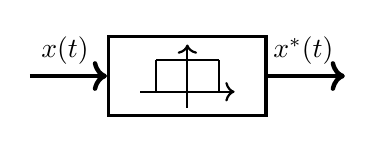
\begin{tikzpicture}[scale=2]

        \node[nblock](aa)at(3.5,-0.5){};
        \draw[->, thick](3.2,-0.6)--(3.8,-0.6);
        \draw[->, thick](3.5,-0.7)--(3.5,-0.3);
        \draw[-,thick](3.3,-0.4)--(3.7,-0.4);
        \draw[-,thick](3.3,-0.4)--(3.3,-0.6);
        \draw[-,thick](3.7,-0.4)--(3.7,-0.6);
        \draw[->,ultra thick](2.5,-0.5)node[above right]{$x(t)$}--(aa.180);
        \draw[->,ultra thick](aa.0)--(4.5,-0.5)node[above left]{$x^*(t)$};

    \end{tikzpicture}
\end{center}

Si può osservare che il filtro in frequenza è $rect\left(\displaystyle\frac{2\omega}{\omega_c}\right)$, per cui riportandolo nel dominio del tempo con un'anti-trasformata di Fuorier si ottiene una $sinc$ nel tempo: 
\begin{equation}
    h(t)=\displaystyle\frac{sin\left(\displaystyle\frac{\omega_c}{2}t\right)}{\displaystyle\frac{\omega_c}{2}t}
\end{equation}
\begin{center}
    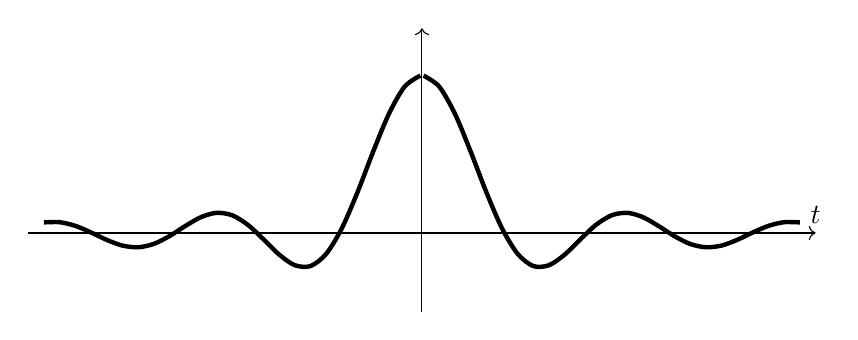
\begin{tikzpicture}[scale=2]
        \draw[->](-2.5,0)--(2.5,0)node[above]{$t$};
        \draw[->](0,-0.5)--(0,1.3);
        \draw[-,ultra thick]plot[smooth,domain=-2.4:-0.01](\x,{sin(6*\x r)/(6*\x)});
        \draw[-,ultra thick]plot[smooth,domain=0.01:2.4](\x,{sin(6*\x r)/(6*\x)});

    \end{tikzpicture}
\end{center}

Ma questa risposta impulsiva è diversa da zero anche per tempi negativi, per cui comincia ad oscillare prima di un entrata, di conseguenza è anticausale. Inoltre 
se viene computata una convoluzione si osserveranno segnali futuri. Per cui non si può lavorare con questo filtro ideale, usato da Shannon nella sua teoria. 

Ma se sono già 
noti tutti i campioni è possibile ricostruire il segnale, poiché si conoscone tutte le entrate future. L'uscita sarà una sommatoria di risposte impulsive, moltiplicate per 
la rispsosta impulsiva del filtro passa-basso, sommando punto per punto si ottiene in uscita il segnale continuo di partenza. Per eseguire questa operazione su un 
processore, si considera una frequenza di campionamento maggiore, quindi si inseiscono altri impulsi tra i campioni noti, ricavati dalle $sinc$. Alternativamente, poiché 
l'effetto della $sinc$ diminuisce nella distanza dal campione, per cui il processore calcola un certo numero di $sinc$ in avanti e le somma a quelle passate per ottenere 
il valore in quel punto. Il numero di $sinc$ che precalcola il processore dipende interamente dalla sua velocità nel calcolarle, poiché deve elaborare il segnale in uscita 
in un tempo minore del tempo di campionamento, altrimenti non sarà possibile riprodurre il segnale. Più $sinc$ in avanti si calcola il 
processore, più aumenta la qualità dell'audio corregendo il valore del campione in quel punto. 

Nel caso di controllori automatici, invece non sono noti campioni futuri, per cui anche un piccolo ritardo può generare un'elevata perdita di fase per il controllore, 
non permettendo il controllo adeguato del sistema. 

Il teorema di Shannon prevede un ricostruttore ideale ovvero è applicabile se e solo se i lobi non si intersecano, in caso contrario si campiona una parte minore del 
lobo centrale e la parte rimanente crea delle distorsioni nel campione di partenza. Questi disturbi sono delle frequenze che non esistevano, sono degli alias creati a causa 
della frequenza di campionamento troppo piccola, per cui questo fenomeno viene chiamato aliasing. Ad alte frequenze vengono misurati valori corrispondenti a basse 
frequenze del polo successivo, ed a basse frequenze vengono misurati contributi del polo precedente ad alte frequenze. 

\begin{center}
    \begin{tikzpicture}[scale=1.2]
        \draw[->](-5,0)--(5,0)node[above]{$\omega$};
        \draw[->](0,-0.25)--(0,1.5)node[right]{$|X_c(j\omega)|$};

        \draw[ultra thick]plot[smooth, domain=0:1.513](\x,{1-0.25*e^(2.7*(\x-1))});
        \draw[ultra thick]plot[smooth, domain=-1.513:0](\x,{1-0.25*e^(-2.7*(\x+1))});

        \draw[ultra thick]plot[smooth, domain=-2.5:-0.987](\x,{1-0.25*e^(2.7*(\x+1.5))});
        \draw[ultra thick]plot[smooth, domain=-4.013:-2.5](\x,{1-0.25*e^(-2.7*(\x+3.5))});

        \draw[ultra thick]plot[smooth, domain=2.5:4.013](\x,{1-0.25*e^(2.7*(\x-3.5))});
        \draw[ultra thick]plot[smooth, domain=0.987:2.5](\x,{1-0.25*e^(-2.7*(\x-1.5))});

        \draw[-,ultra thick, blue](1.25,0)--(1.25,1)--(-1.25,1)--(-1.25,0);

        \filldraw[black](1.25,0)node[below]{$\displaystyle\frac{\omega_c}{2}$}circle(0.5pt);
        \filldraw[black](-1.25,0)node[below]{$\displaystyle-\frac{\omega_c}{2}$}circle(0.5pt);
        \filldraw[black](2.5,0)node[below]{$\omega_c$}circle(0.5pt);
        \filldraw[black](-2.5,0)node[below]{$-\omega_c$}circle(0.5pt);
        \filldraw[black](3.75,0)node[below]{$\displaystyle\frac{3\omega_c}{2}$}circle(0.5pt);
        \filldraw[black](-3.75,0)node[below]{$\displaystyle-\frac{3\omega_c}{2}$}circle(0.5pt);
        \filldraw[black](0,0)node[below right]{$0$}circle(0.5pt);
  
    \end{tikzpicture}
\end{center}

Il fenomeno dell'aliasing può verificarsi anche per la riproduzione delle immagini, è quindi un problema informatico e dipende dal fatto che le informazioni digitali sono 
discrete, ed ogni volta che dovranno rappresentare qualcosa di continuo sarà presente un fenomeno di aliasing. 

Per evitare l'aliasing si ignorano queste frequenze usando un filtro anti-aliasing a monte del campionatore. Questo filtro, proprio perché l'aliasing è un fenomeno comune 
ad ogni fenomeno digitale, è sempre presente. Alle volte viene realizzato digitalmente, può essere implementato un sistema che campiona ad una frequenza maggiore per pulire 
il segnale e poi lo passa al campionatore. 

Un algoritmo di controllo per aumentare la frequenza costa molto, mentre è più economico aumentare la frequenza del campionatore. Altrimenti si può inseire un circuito formato 
da condensatori e resistenze, per realizzare un filtro anti-aliasing elettronico. 

\subsection{Organo di Tenuta}

Data una sequenza di campioni da ricostruire nella $DAC$ non si possono sommare tutte le $sinc$, poiché comprendono una parte anti-causale, e richiederebbe troppo tempo. 
Poiché non è possibile usare il ricostruttore ideale di Shannon in questa situazione, si considerano ricostruttori semplificati, più veloci e meno precisi. 

Se si usa un ricostruttore semplificato, diverso da quello di Shannon, diminuirà il tempo necessario per elaborare 
i dati, ma diminuirà la precisione del segnale in uscita. Il più semplice ricostruttore possibile è composto 
da una gradinata che assume tensione costante per ogni intervallo di campionamento, definito ricostruttore di ordine zero o tenuta di ordine zero. 

\begin{center}
    \begin{tikzpicture}[scale=3]
        \draw[->](-0.25,0)--(1.5,0)node[above]{$t$};
        \draw[->](0,-0.25)--(0,1)node[right]{$x(t)$};

        \filldraw[black](0,0.6)circle(0.5pt);
        \filldraw[black](0.2,0.7)circle(0.5pt);
        \filldraw[black](0.4,0.8)circle(0.5pt);
        \filldraw[black](0.6,0.7)circle(0.5pt);
        \filldraw[black](0.8,0.6)circle(0.5pt);
        \filldraw[black](1,0.5)circle(0.5pt);
        \filldraw[black](1.2,0.6)circle(0.5pt);

        \draw[-,very thick](0,0.6)--(0.2,0.6);
        \draw[-,very thick](0.2,0.7)--(0.4,0.7);
        \draw[-,very thick](0.4,0.8)--(0.6,0.8);
        \draw[-,very thick](0.6,0.7)--(0.8,0.7);
        \draw[-,very thick](0.8,0.6)--(1,0.6);
        \draw[-,very thick](1,0.5)--(1.2,0.5);
        \draw[-,very thick](1.2,0.6)--(1.4,0.6);

        \draw[dashed](0.2,0.7)--(0.2,0)node[below]{$T_c$};
    \end{tikzpicture}
\end{center}

Una tenuta di orine uno invece è composta da rampe ogni tempo di campionamento che congiungono due campioni diversi. In queste analisi non si considereranno tenute di 
ordine superiore, per cui si utilizzza un $ZOH$, $Zero\:\:Order\:\:Holder$.

Per calcolare l'errore dovuto ad una tenuta di ordine $0$ si analizza la sua funzione di trasferimento. Il segnale ricostruito con questo ricostruttore sarà:
\begin{equation}
    x^*(t)=\sum_{k=0}^{+\infty}x_k(\delta_{-1}(t-kT_c)-\delta_{-1}(t-(k+1)T_c))
\end{equation}
\begin{center}
    \begin{tikzpicture}[scale=3]
        \draw[->](-0.25,0)--(1.5,0)node[above]{$t$};
        \draw[->](0,-0.25)--(0,1)node[right]{$x(t)$};

        \filldraw[black](0,0.6)circle(0.5pt);
        \filldraw[black](0.2,0.7)circle(0.5pt);
        \filldraw[black](0.4,0.8)circle(0.5pt);
        \filldraw[black](0.6,0.7)circle(0.5pt);
        \filldraw[black](0.8,0.6)circle(0.5pt);
        \filldraw[black](1,0.5)circle(0.5pt);
        \filldraw[black](1.2,0.6)circle(0.5pt);

        \draw[-,very thick](0,0.6)--(0.2,0.6);
        \draw[-,very thick](0.2,0.7)--(0.4,0.7);
        \draw[-,very thick](0.4,0.8)--(0.6,0.8);
        \draw[-,very thick](0.6,0.7)--(0.8,0.7);
        \draw[-,very thick](0.8,0.6)--(1,0.6);
        \draw[-,very thick](1,0.5)--(1.2,0.5);
        \draw[-,very thick](1.2,0.6)--(1.4,0.6);

        \draw[-, thick](0.4,0.8)--(0.4,0)node[below left]{$kT_c$};        
        \draw[-, thick](0.6,0.8)--(0.6,0)node[below]{$(k+1)T_c$};
        \draw[dashed](0.4,0.8)--(0,0.8)node[left]{$x_k$};

    \end{tikzpicture}
\end{center}

Avrà una funzione di trasferimento: 
\begin{equation}
    X^*(s)=\sum_{k=0}^{+\infty}x_k\left(\displaystyle\frac{1}{s}e^{-kT_cs}-\frac{1}{s}e^{-(k+1)T_cs}\right)=\sum_{k=0}^{+\infty}x_ke^{-kT_cs}\left(\frac{1-e^{-T_cs}}{s}\right)
\end{equation}

Il primo termine corrisponde alla funzione di trasferimento del segnale campionato:
\begin{gather}
    X_c(s)=\sum_{k=0}^{+\infty}x_ke^{-kT_cs}\\
    X^*(s)=X_c(s)\left(\displaystyle\frac{1-e^{-T_cs}}{s}\right)
\end{gather}
L'organo di tenuta di ordine zero avrà funzione di trasferimento: 
\begin{equation}
    T(s)=\displaystyle\frac{1-e^{-T_cs}}{s}
\end{equation}
Questo organo di tenuta può essere rappresentato come un blocco funzionale in cui entra il segnale campionato come sequenza di impulsi ed esce il segnale ricostruito a gradino. 
Questa funzione sembra avere un integratore, ma non è un rapportro tra polinomi. Per controllore quale dinamica prevale si considera un'approssimazione dell'esponenziale, per 
$s$ a basse frequenze: 
\begin{gather}
    e^{-T_cs}=\displaystyle\frac{1}{e^{T_cs}}\approx\frac{1}{1+T_cs}\\
    T(s)\approx\displaystyle\frac{1-\displaystyle\frac{1}{1+T_cs}}{s}=\frac{1}{s}\frac{1+T_cs-1}{1+T_cs}=\frac{T_c}{1+T_c}s
\end{gather}
Per cui ha un guadagno $T_c$, ed è una funzione di trasferimento del primo ordine ad avrà il seguente andamento:
\begin{center}
    \begin{tikzpicture}[scale=2]
        \draw[->](-0.25,0)--(2,0)node[above]{$\omega$};
        \draw[->](0,-0.25)--(0,1.5)node[right]{$|T(j\omega)|$};

        \node[left]at(0,1){$T_c$};
        \draw[-,very thick,blue](0,1)--(1.3,1)--(1.9,-0.3)node[right]{$ZOH$};
        \draw[dashed,blue](1.3,1)--(1.3,0)node[below]{$\displaystyle\frac{1}{T_c}$};
        \draw[-,very thick, green](0,1.02)--(1.6,1.02)--(1.6,0)node[below]{$\displaystyle\frac{\pi}{T_c}$};

        \filldraw[black](0.8,0)node[below]{$\omega_m$}circle(0.5pt);
    \end{tikzpicture}
\end{center}
La banda passante di questo sistema con un unico polo a $\displaystyle\frac{1}{T_c}$ coincide con questo polo. Per il ricostruttore di Shannon, la banda passante è esattamente 
$\displaystyle\frac{\omega_c}{2}=\frac{\pi}{T_c}$. Nel caso reale il modulo scende di $20\:dB$ ogni decade, per quello ideale di Shannon il modulo scende in maniera secca. 
Per cui la frequenza massima da campionare $\omega_m$ deve essere necessariamente minore di $\displaystyle\frac{1}{T_c}$. Per un ricostruttore ideale ipotizzato da Shannon 
è sufficiente che la pulsazione di campionamento sia il doppio della pulsazione massima da campionare. Con un ricostruttore ideale la pulsazione di campionamento deve essere 
minimo $10$ o $20$ volte la pulsazione massima da campionare, ancora meglio se la pulsazione di campionamento è $100$ volta della pulsazione massima, anche se può essere 
troppo. Per cui una pulsazione di campionamento doppia rispetto a $\omega_m$ ricade solo nel domino ideale. 

Per cui il tempo di campionameto va scelto in base alle tipologie di frequenza che si vogliono campionare. Per alcuni sistemi il tempo di campionamento deve essere variabile, 
mentre per altri deve rimanere costante. 


Il sistema potrebbe essere misurato da sensori analogi o digitali, in questo caso si avrà una misura discretizzata. Questi encoder possono essere realizzati da un disco 
forato in rotazione, dei fototransistor possono percepire la luce che passa attravaraso i fori del disco in un intervallo di tempo generando un'onda quadra in uscita con 
frequenza proporzionale alla velocità di rotazione del disco. La luce fornisce una piccola differenza di potenziale per attivare il transistor, composto da una coppia 
foto diodo, generando l'onda. Con il fronte di salita si può incrementare un clock oppure si può creare un segnale periodico per controllare il processo. 
Può presentare un'altra corona più interna con un'altra coppia fotodiodo e fototransistor per ottenere il doppio degli impulsi da usare, possono essere usati in un semplice 
circuito per determinare il verso di rotazione del disco, agendo come uno XOR. 
Ponendo i fototransistor uno prima dell'altro, se il circuito ruota un senso il fronte di salita di uno dei due verrà prima del secondo e viceversa, in questo modo 
sapendo la posizione dei fototransistor è possibile determinare il verso di rotazione. 
Questi encoder sono utilizzati quando si accende un sistema, senza sapere la posizione in cui si trova. Può anche essere presente un foro centrale in grado di 
resettare la misura. 
%\begin{center}
%    \includemovie{Fototransistor.gif}
%\end{center}

\subsection{Equazione alle Differenze}

Un'equazion differenziale che implementa un controllore $C(s)$ non può essere rappresentata in un dominio discreto, poiché il controllore lavora con una sequenza di valori 
$\{u_k\}$ in entrata, legati ognugno ad un tempo $kT_c$. Esiste un altro modello di equazione che descrivono come le equazioni differenziali sistemi con memoria, sono chiamate 
equazioni alle differenze. In un equazione alle differenze un uscita $y_{k+1}$ dipende da tutti i valori precedenti di entrata e uscita, per cui rappresenta un sistema con 
memoria: 
\begin{equation}
    y_{k+1}=g\left(\{y_k\},\{u_k\}\right)
\end{equation}
Per cui è possibile rappresentare un sistema dinamico con un'equazione alle differenze. Il grado $n$ di un'equazione alle differenze è determinato dalla distanza dall'elemento 
calcolato dalla sequenza fornita, ovvero è determinato dal massimo numero sommato al pedice $y_{k+n}$. 

I valori iniziali di un'equazione alle differenze sono corrispondenti alle condizioni iniziali di un'equazione differenziale. In questo caso si considera un'equazione di grado 
$1$ poiché si sintetizza lo stato del sistema da $k=0$, data la sequenza di campioni $\{u_K\}$ è necessario inizializzare il sistema fornendo il valore $y_0$. 
Si ha:
\begin{gather}
    y_1=g(y_0,\{u_k\})\\
    y_2=g(y_1,y_0,\{u_K\})\\
    \vdots\\
    y_{k+1}=g(\{y_k\},\{u_k\})
\end{gather}

Tramite 
quesra equazione si ossevano valori in entata ed in uscita solo in istanti discreti. Per cui questo oggetto genera una sequenza $\{y_k\}$, da un entrata $\{u_k\}$, prodotta 
da un'equazione con menoria, ovvero dipende dalla storia del sistema, descriverà un sistema dinamico. 

\begin{center}\begin{tikzpicture}[scale=2]
    \node[rectangle, draw, very thick, minimum width=2cm, minimum height=1cm](r)at(0,0){$g(\{y_k\},\{u_k\})$};

    \draw[->,ultra thick](-1,0)--(r.west);
    \node[below]at(-0.8,0){$\{u_k\}$};

    \draw[<-,ultra thick](1,0)--(r.east);
    \node[below]at(0.8,0){$\{y_k\}$};

\end{tikzpicture}\end{center}

Questa equazione può essere implementata facilmente su un computer poiché è un'operazione ricorsiva.Un microprocessore può simulare un'equazione alle differenze in base ai 
dati in entrata e così calcolarsi il controllore per ogni tempo di campionamento, questo calcolo 
verrà inviato al 
convertitore $DAC$. Dopo aver inviato i dati in uscita, il microcontrollore aspetterà la fine del tempo di campionamento prima di eseguire nuovamente il calcolo 
del controllore. 

\subsection{Trasformata $Z$}

Supponiamo di avere una successione di valori $y[k]$, si definisce la trasformata $Z$ per questa sequenza di valori:
\begin{gather}
    Z\{y[k]\}=y[0]+y[1]z^{-1}+y[2]z^{-2}+\cdots+y[k]z^{-k},\mbox{ per }k\to+\infty\\
    Y(z)=\sum_{k=0}^{+\infty}y[k]z^{-k}
\end{gather}
Per determinarne la convergenze si manipola per farla assomigliare ad una serie geometrica. 

Si considera un segnale in entrata $e^{pt}$ con $p<0$, campionandolo si ottiene una sequenza di valori $\{e^{pkT_c}\}$, si applica quindi la trasformaza $Z$ ai campioni 
ottenuti dall'esponenziale:
\begin{equation}
    Z\{e^{pkT_c}\}=\sum_{k=0}^{+\infty}e^{pkT_c}z^{-k}=\sum_{k=0}^{+\infty}\left(e^{pT_c}z^{-1}\right)^k
\end{equation}
Una serie geometrica del tipo $\sum x^k$ converge a $\displaystyle\frac{1}{1-x}$ se $|x|<1$ ovvero considerando $x\in\mathbb{C}$ il valore $x$ deve rimanre all'interno 
di una circonferenza unitaria avente centro nell'origine del piano di Gauss. Per cui la trasformata $Z$ sarà: 
\begin{equation}
    |e^{pT_c}z^{-1}|<1\Rightarrow Z\{e^{pkT_c}\}=\displaystyle\frac{1}{1-e^{pT_c}z^{-1}}=\frac{z}{z-e^{pT_c}}
\end{equation}
Il componente $e^{pT_c}z^{-1}$ corrisponde all'integrale discreto di $e^{pT_c}$, equivalente ad una sommatoria. Considerando una circonferenza di centrata nell'origine 
del piano gi Gauss ri raggio $|e^{pT_c}|$, quando $|z|>|e^{pT_c}|$ si avrà $|e^{pT_c}z^{-1}|<1$, per cui convergerà per ogni all'esterno di questa frontiera. 
Analogamente alla trasformata di Laplace, che converge a destra di un'ascissa di Laplace $s=s_0$, coincidente il polo. 

Lo stesso elemento $e^{pt}$ in Laplace diventa $\displaystyle\frac{1}{s+p}$, mentre in $Z$ diventa $\displaystyle\frac{z}{z-e^{pT_c}}$, con $p<0$. Il polo in Laplace 
viene rappresentato come $p$, mentre in $Z$ come $e^{pT_c}$. Per $p=0$, si ha un gradino e la sua trasformata $Z$ sarà:
\begin{equation}
    Z\{\delta_{-1}[t]\}=\displaystyle\frac{z}{z-1}
\end{equation}


Dato un segnale $\{y_k\}$, la sua trasformata $Z$ sarà data da una somma di segnali ritardati. Moltiplicando per un fattore $z^{-1}$ l'intera sequenza è come se si analizzasse 
un segnale il cui primo elemento campionato sia nullo, per cui si ritarda il segnale. 
\begin{gather}
    Z\{y_k\}=y_0+y_1z^{-1}+y_2z^{-2}+\cdots\\
    0+y_0z^{-1}+y_1z^{-2}+y_2z^{-3}+\cdots=Z\{y_k\}\cdot z^{-1}=Z\{y'_k\}
\end{gather}
Questo tipo di ritardo viene chiamato ritardo elementare, non è un ritardo nel dominio del tempo, ma un ritardo nella sequenza di campioni. 


Data una trasformata $Z$ $Y(z)=\displaystyle\sum_{k=0}^{+\infty}(e^{pT_c}z^{-1})^k$, per ottenere il valore finale si considera:
\begin{equation}
    Y(\infty)=\lim_{z\to1}\displaystyle\frac{z-1}{z}Y(z)
\end{equation}
Per ottenere $1$ per $z^{-1}$ bisogna porre $p=0$, per cui si calcola il valore finale nel piano $Z$ per $z\to1$. Nel continuo il polo è in $0$, mentre nel discreto è in 
$e^{0\cdot T_c}=1$.  


Data un'equazione alle differenze: 
\begin{equation}
    y_{k+1}=ay_k+bu_k
\end{equation}
Si considerano le sequenze $\{y_k\}$ e $\{u_k\}$ come se fossero ritardate di un campione per cui $\{y_{k+1}\}=\{y_k\}$, tenendo conto del ritardo che si ha si riscrive come:
\begin{gather}
    \{y_k\}=a\{y_k\}'+b\{u_k\}'\\
    Y(z)=aY(z)z^{-1}+bU(z)z^{-1}\\
    Y(z)z=aY(z)+bU(z)\Rightarrow \displaystyle\frac{Y(z)}{U(z)}=W(z)=\displaystyle\frac{b}{z-a}
\end{gather}
Per cui questa funzione descriverà il sistema dinamico descritto da quella equazione alle differenze. 

Si potrebbe quindi implementare un controllore per un'equazione alle differenze se si riuscisse a traspostarlo dal dominio di Laplace al dominio $Z$. 

\subsection{Mapping dal Piano $s$ a $z$}

Dato un segnale $x(t)$ campionato $x_c(t)=\displaystyle\sum_{k=0}^{+\infty}x_k\delta_0(t-kT_c)$, può essere applicata sia una trasformata di Laplace che una trasformata $Z$, per 
cui si ha:
\begin{gather}
    X_c(s)=\sum_{k=0}^{+\infty}x_ke^{-skT_c}\\
    X_c(z)=\sum_{k=0}^{+\infty}x_kz^{-k}
\end{gather}
Si può sostituire $z\to e^{sT_c}$ per ottenere la trasformata di Laplace partendo dalla trasformata $Z$, ma non rappresenta una relazione di eguaglianza tra le due. 
Ma dovranno comunque essere collegati in qualche modo. Per cui si analizza al variare della pulsazione naturale di $s$, il l'effetto percepito nel piano $Z$. 

Si considera un'unica striscia nell'intervallo $\left[\displaystyle-j\frac{\omega_c}{2},j\frac{\omega_c}{2}\right]$, poiché la trasformata è periodica, nel solo semipiano 
negativo, poiché si vuole analizzare il comportamento di sistemi stabili. 

Considerando la risposta armonica in Laplace, si avrà $s=j\omega$, per cui si avrà una relazione: $z=e^{j\omega T_c}=e^{2\pi j\frac{\omega}{\omega_c}}$. 

Per la risposta armonica all'aumentare della pulsazione naturale, in positivo o in negativo, 
allora si compierà una rotazione nel dominio $z$ fino ad un valore $2\pi j\displaystyle\frac{\left(\frac{\pm\omega_c}{2}\right)}{\omega_c}=\pm j\pi$, per cui si avrà una rotazione di 
$180^{\circ}$ in senso orario per pulsazioni naturali negative, e in senso antiorario per pulsazioni naturali positive. Queste rotazioni formeranno una circonferenza 
unitaria. 

L'origine del piano di Laplace coincide con il punto $z=e^{j0T_c}=1$, per $s$ puramente reale, sarà puramente reale anche il corrispettivo in $z$, per cui il semiasse 
negativo dell'asse dei reali coincide con il segmento dal punto $1$ all'origine degli assi in $z$. 

Per $s=\sigma+j\omega$, dovrà avere necessariamente parte reale negativa per rappresentare un sistema stabile, per cui si avrà $\sigma\in(-\infty,0]$, quindi 
$z=e^{2\pi\frac{(\sigma+j\omega)}{\omega_c}}=e^{2\pi\sigma}e^{2\pi j\frac{\omega}{\omega_c}}$, poiché $\sigma$ è necessariamente negativo questo risulterà in 
delle rotazioni intorno all'origine dell'asse $z$, con raggio $e^{2\pi\sigma}<1$. Per cui corrisponderà a delle circonferenze concentriche di raggio decrescente al 
diminuire di $\sigma$. 

Si può definre una nuova condizione di stabilità per il dominio $z$ poiché tutti i poli avente parte reale negativa sono contenuti nella circonferenza 
unitaria centrata nell'origine degli assi. Tutti i poli contenuti in questa circonferenza daranno origine a delle dinamiche stabili, mentre i poli sulla circonferenza unitaria 
saranno al limite di stabilità, invece tutti i poli esterni saranno instabili. 

\begin{center}
    \begin{tikzpicture}[scale=2]
        \draw[->,very thick](-2,0)--(0.5,0)node[above]{$\Re(s)$};
        \draw[->,very thick](0,-1)--(0,1)node[right]{$\Im(s)$};

        \draw[->,very thick, red](0,0)--(0,0.5)node[right,black]{$\displaystyle j\frac{\omega_c}{2}$};       
        \draw[->,very thick, red](0,0)--(0,-0.5)node[right,black]{$\displaystyle-j\frac{\omega_c}{2}$};
        
        \draw[->,very thick,cyan](0,0.5)--(-1.9,0.5)node[above right,black]{$a$};
        \draw[->,very thick,cyan](0,-0.5)--(-1.9,-0.5)node[below right,black]{$b$};

        \draw[->,very thick, blue](0,0)--(-1.9,0);

        \filldraw[black](0,0)circle(1pt);

        \draw[->,ultra thick](0.7,0)node[above right]{$z=e^{sT_c}$}--(2,0);

    \end{tikzpicture}
    \begin{tikzpicture}[scale=2]
        \draw[->,very thick](-1,0)--(1,0)node[above]{$\Re(z)$};
        \draw[->,very thick](0,-1)--(0,1)node[right]{$\Im(z)$};

        \draw[<-,very thick, red]plot[smooth, domain=-0.5:0.5](\x,{(0.25-(\x)^2)^0.5});
        \draw[<-,very thick, red]plot[smooth, domain=-0.5:0.5](\x,{-(0.25-(\x)^2)^0.5});

        \draw[->,very thick, blue](0.5,0)--(0,0);

        \draw[<-,very thick, cyan](0,0)node[above left,black]{$a$}node[below left,black]{$b$}--(-0.5,0);

        \filldraw[black](0.5,0)node[above right]{$1$}circle(1pt);
    \end{tikzpicture}
\end{center}

Più il raggio della circonferenza dove si trovano i poli è piccolo, maggiore è lo smorzamento dei poli. Due poli complessi e coniugati vengono rappresentati simmetricamente 
anche nel piano $z$. Dato un polo su una circonferenza se la percorre in senso antiorario nel semipiano immaginario positivo, oppure in senso orario nel semipiano immaginario 
negativo, allora il suo smorzamento diminuisce ed aumenta la sua pulsazione naturale. Se un polo su una circonferenza si sposta radialemente su un'altra di raggio maggiore 
allora il suo smorzamento aumenta e la sua pulsazione naturale rimane invariata.  

Data una funzione di trasferimendo in $z$ avente un polo $p$ nel segmento $a/b$ su $z$:
\begin{equation}
    W(z)=\displaystyle\frac{1}{z+p}
\end{equation}
Questa funzione non può esistere nel dominio di Laplace poiché quel punto corrisponde a due punti complessi e coniugati in $s$, per cui nel mondo del discreto si possono 
descrivere oggetti che non possono esistere nel continuo. Si può rappresentare come un'equazione alle differenze $y_{k+1}=-|p|y_k+u_k$, per un'entrata $u_0=0$ e $y_0=1$, 
allora si avrà una conversione alternante che converge a zero alternando. Questa successione non deriva da nessun campionamento di un sistema lineare, quindi è un oggetto 
esclusivo al discreto. 

Poiché la trasformata $Z$ è una serie, bisogna determinare la sua convergenza. Data una serie $\displaystyle\sum_{k=0}^{+\infty}a_k$ questa converge in assoluto, se rispetta il 
criterio di convergenza assoluta:
\begin{quotation}
    Una serie $\displaystyle\sum_{k=0}^{+\infty}a_k$ converge in assoluto, ovvero converge la serie $\displaystyle\sum_{k=0}^{+\infty}|a_k|$, se il rapporto tra un termine della serie ed il precedente 
    è definitivamente di modulo strettamente minore di uno dopo un valore $k_0$: $\displaystyle\left|\frac{a_{k+1}}{a_k}\right|<1,\:k\geq k_0$.
\end{quotation}
Per cui se il modulo degli elementi della serie diminuiscono strettamente allora la serie non può che convergere. 

Data $X(z)=\sum_{k=0}^{+\infty}x_kz^{-k}$, è convergente in assoluto se:
\begin{gather}
    \left|\displaystyle\frac{x_{k+1}}{x_k}\right|<1\\
    x_{k+1}=\alpha x_k+u_k\\
    \left|\displaystyle\frac{x_{k+1}}{x_k}\right|=|\alpha|<1,\mbox{ per }u_k=0
\end{gather}
Per cui il sistema converge in assoluto se il polo è interno alla circonferenza unitaria, quindi la sua trasformata $Z$ può essere espressa come:
\begin{equation}
    W(z)=\displaystyle\frac{1}{z-\alpha}
\end{equation}

\subsection{Trasformazioni $s\to z$}

Poiché è possibile passare da uno stesso segnale nel tempo al dominio di Laplace ed al dominio $Z$ separatamente. Per cui si vuole trovare un modo per passare direttamente 
dal dominio di Laplace al dominio $Z$ senza ritornare al segnale originale nel tempo. Discretizzando un sistema bisogna scegliere il tempo di campionamento adeguato. Ritardare 
un segnale discreto di poco può causare una destabilizzazione del sistema a ciclo chiuso, per cui il tempo di campionamento è necessario che sia molto preciso 

Considerando un sistema a controreazione:
\begin{center}\begin{tikzpicture}[scale=2]
    \coordinate(sum)at(-1,0){};
    \node[block, right of=sum, node distance=2cm](c){$C(s)$};

    %\draw[->,ultra thick](sum.0)--(c.180);
    \filldraw[black](2.5,0)circle(1pt);

    \draw[->,ultra thick](2.5,0)node[above right]{}--(3,0);
    \draw[-,ultra thick](2.5,-0.75)--(2.5,0);

    %\node[block]at(0.75,-0.75)(h){$H(s)$};
    \node[block]at(1.75,0)(p){$P(s)$};

    \draw[-,ultra thick](p.0)--(2.5,0);
    \draw[->,ultra thick](c.0)node[above right]{}--(p.180);

    %\draw[->,ultra thick](2.5,-0.75)--(h.0);
    %\draw[-,ultra thick](h.180)--(-1,-0.75);
    \draw[-,ultra thick](2.5,-0.75)--(0,-0.75);
    \draw[->,ultra thick](0,-0.75)--(c.270);
\end{tikzpicture}\end{center} 
Il processo $P(s)$ può essere espresso nel discreto, ma il controllore $C(s)$ creato nel continuo bisogna trasportarlo nel discreto. 
Una volta ottenuta la funzione $C(z)$ si può implementare l'equazione alle differenze tramite cicli implementati per mezzo di $interrupt$ in modo che il sistema operativo 
non blocchi l'esecuzione del controllore senza che questo blocchi l'esecuzione del sistema operativo. 

\subsubsection{Trasformazione Esatta e Guadagno}

Passando per il domino del tempo è sempre possibile trasformare una funzione continua in una discreta. Scomponendo il controllore in poli e 
residui, trasportando ogni residuo nel discreto separatamente:
\begin{gather}
    C(s)=\displaystyle\sum_{i=0}^{n}\frac{R_i}{s+p_i}\\
    C(z)=\displaystyle\sum_{i=0}^{n}\frac{R_i}{z+e^{p_iT_c}}
\end{gather}
Questa trasformazione viene chiamata trasformazione esatta, ed il polo si sposta da $p_i$ a $e^{p_iT_c}$. Il guadagno in Laplace si ottiene ponendo $s=0$, quindi sarà: 
$\displaystyle\frac{R_i}{p_i}$, per la trasformata $Z$, si pone $z=0$ corrisponde ad un valore di $s=1$, sarà: $\displaystyle\frac{R_i}{e^{p_iT_c}}$. Sorge un problema 
poiché avranno la stessa risposta impulsiva, ma hanno una risposta al gradino diversa, su cui si calcola il gaudagno. Il guadagno così ottenuto dipenderà anche dal tempo 
di campionamento scelto, per cui non la trasformazione esatta non è usata. 

Per avere la stessa risposta al gradino si potrebbe 
moltiplicare la trasformata $Z$ di ogni residuo per un fattore $\displaystyle\frac{e^{p_iT_c}}{p_i}$, in modo da avere la stessa risposta al gradino. Questa trasformazione 
viene chiamata trasformazione al guadagno. Ma in questo modo 
avranno una risposta uguale solo ad un'entrata a gradino, per cui questo metodo non viene mai utilizzato. Non esiste una trasformazioine "giusta" esistono sono delle 
approssimazioni, ed alcune sono più soddisfacienti delle altre in determinate situazioni.  

\subsubsection{Trasformazione ZOH}

Si considera invece di discretizzare la funzione direttamente si moltiplica per l'organo di tenuta e in seguito si applica la trasformata $Z$, allora si avrà:
\begin{gather}
    Z\left[C(s)T(s)\right]=Z\left[C(s)\displaystyle\frac{1-e^{sT_c}}{s}\right]\\
    Z\left[\displaystyle\frac{C(s)}{s}\right]-Z\left[\displaystyle\frac{C(s)}{s}e^{-sT_c}\right]\\
    Z\left[\displaystyle\frac{C(s)}{s}\right](1-z^{-1})
\end{gather}
Per cui il segnale sarà ritardato di un campione poiché $e^{-sT_c}$ rappresenta un ritardo nel discreto di un campione. 

\subsubsection{Trasformazione di Tustin}

Per determinare la discretizzazione migliore per una data situazione bisogna analizzare il diagramma di Bode e controllare quale discretizzazione ha una risposta più simile 
al controllore continuo, oppure si controllare quale controllore ha una risposta al gradino più simile, oppure si usano metodi diversi in base ai risultati richiesti. 
La trasformazione di Tustin viene chiamata trasformazione approsimata. 

Data una curva, e noto il valore dell'integrale $y_k$ della curva fino ad un punto $kT_c$, si può approssimare il valore dell'integrale $y_{k+1}$ ad un punto successivo 
$(k+1)T_c$, come un'equazione alle differenze dato il campione nel punto $kT_c$ oppure nel punto successivo $(k+1)T_c$:
\begin{gather}
    i)\:y_{k+1}=y_k+T_cu_k\\
    ii)\:y_{k+1}=y_k+T_cu_{k+1}
\end{gather}
Dove il $u_k$ è il valore del campione nell'intervallo di campionamento $kT_c$, per cui si approssima la curva come una serie di rettangoli, in questo modo in base 
a quale campione si sceglie per approsismare il rettangolo si avrò un'approssimazione maggiore o minore del valore reale dell'integrale. Un'approssimazione di questo tipo 
però non è molto precisa, per cui invece di un rettangolo si considera un trapezio di basi $u_k$ e $u_{k+1}$ e altezza $T_c$ di area $(u_k+u_{k+1})\displaystyle\frac{T_c}{2}$. 
Questa approssimazione viene chiamata approssimazione di Tustin, ed avrà un'equazione alle differenze:
\begin{equation}
    iii)\:y_{k+1}=y_k+(u_k+u_{k+1})\displaystyle\frac{T_c}{2}
\end{equation}

\begin{center}
    \begin{tikzpicture}[scale=2.9]
        \draw[fill=cyan](0.4,1.141)--(0.8,1.141)--(0.8,0.6)--(0.4,0.6)--(0.4,1.141);

        \draw[->](0,0.5)--(0,1.5)node[right]{$x(t)$};
        \draw[->](-0.25,0.6)--(1,0.6)node[above]{$t$};

        \draw[]plot[smooth, domain=-0.2:1](\x,{1+0.2*sin(2*\x r)});
        %\draw[->,ultra thick](0,0)node[below left]{$0$}--(0,1);
        \draw[-,ultra thick](0.4,0.6)node[above left]{$kT_c$}--(0.4,1.141);
        \draw[-,ultra thick](0.8,0.6)node[below]{$(k+1)T_c$}--(0.8,1.141);
        \draw[-,ultra thick](0.4,1.141)--(0.8,1.141);
        \draw[-,ultra thick](0.4,0.6)--(0.8,0.6);
        \draw[dashed](0.8,1.199)--(0.8,1.141);


        \draw[dashed](0.4,1.141)--(0,1.141)node[below left]{$u_k$};
        \draw[dashed](0.8,1.199)--(0,1.199)node[left]{$u_{k+1}$};
    \end{tikzpicture}
    \begin{tikzpicture}[scale=2.9]
        \draw[fill=blue](0.4,1.199)--(0.8,1.199)--(0.8,0.6)--(0.4,0.6)--(0.4,1.199);

        \draw[->](0,0.5)--(0,1.5)node[right]{$x(t)$};
        \draw[->](-0.25,0.6)--(1,0.6)node[above]{$t$};

        \draw[]plot[smooth, domain=-0.2:1](\x,{1+0.2*sin(2*\x r)});
        %\draw[->,ultra thick](0,0)node[below left]{$0$}--(0,1);
        \draw[-,ultra thick](0.4,0.6)node[above left]{$kT_c$}--(0.4,1.199);
        \draw[-,ultra thick](0.8,0.6)node[below]{$(k+1)T_c$}--(0.8,1.199);
        \draw[-,ultra thick](0.4,1.199)--(0.8,1.199);
        \draw[-,ultra thick](0.4,0.6)--(0.8,0.6);

        \draw[dashed](0.4,1.141)--(0,1.141)node[below left]{$u_k$};
        \draw[dashed](0.8,1.199)--(0,1.199)node[left]{$u_{k+1}$};
    \end{tikzpicture}
    \begin{tikzpicture}[scale=2.9]
        \draw[fill=red](0.4,1.141)--(0.8,1.199)--(0.8,0.6)--(0.4,0.6)--(0.4,1.141);

        \draw[->](0,0.5)--(0,1.5)node[right]{$x(t)$};
        \draw[->](-0.25,0.6)--(1,0.6)node[above]{$t$};

        \draw[]plot[smooth, domain=-0.2:1](\x,{1+0.2*sin(2*\x r)});
        %\draw[->,ultra thick](0,0)node[below left]{$0$}--(0,1);
        \draw[-,ultra thick](0.4,0.6)node[above left]{$kT_c$}--(0.4,1.141);
        \draw[-,ultra thick](0.8,0.6)node[below]{$(k+1)T_c$}--(0.8,1.199);
        \draw[-,ultra thick](0.4,1.141)--(0.8,1.199);
        \draw[-,ultra thick](0.4,0.6)--(0.8,0.6);


        \draw[dashed](0.4,1.141)--(0,1.141)node[below left]{$u_k$};
        \draw[dashed](0.8,1.199)--(0,1.199)node[left]{$u_{k+1}$};
    \end{tikzpicture}
\end{center}

Si può ottenere l'approssimazione di un integratore $\displaystyle\frac{1}{s}$ tramite la funzione di trasferimento discreta delle equazioni alle differenze:
\begin{gather}
    i)\:y_{k+1}=y_k+T_cu_k\\
    Y(z)=Y(z)z^{-1}+T_cU(z)z^{-1}\\
    W(z)=\displaystyle\frac{T_cz_{-1}}{1-z^{-1}}\approx\frac{1}{s}\\
    s\approx\displaystyle\frac{1}{T_c}\frac{1-z^{-1}}{z^{-1}}\\
    ii)\:y_{k+1}=y_k+T_cu_{k+1}\\
    Y(z)=Y(z)z^{-1}+T_cU(z)\\
    W(z)=\displaystyle\frac{T_c}{1-z^{-1}}\approx\frac{1}{s}\\
    s\approx\displaystyle\frac{1-z^{-1}}{T_c}\\
    iii)\:y_{k+1}=y_k+(u_k+u_{k+1})\displaystyle\frac{T_c}{2}\\
    Y(z)=Y(z)z^{-1}+\displaystyle\frac{T_c}{2}U(z)(1+z^{-1})\\
    W(z)=\displaystyle\frac{T_c}{2}\frac{1+z^{-1}}{1-z^{-1}}\approx\frac{1}{s}\\
    s\approx\displaystyle\frac{2}{T_c}\frac{1-z^{-1}}{1+z^{-1}}
\end{gather}
Quest'ulima approssimazione viene anche chiamata approsimazione bilineare. Poiché $s$ corrisponde ad un derivatore, in questo modo si approssima il derivatore in $z$, ma 
l'accuratezza di questo derivatore cambia radicalmente in base a quale approssimazione si usa. 
Non si può usare la relazione $z=e^{sT_c}$, poiché l'esponenziale non è una realzione lineare, non si potrà mai usare questa trasformazione esatta. 
Considerando l'approssimazione più semplice, ovvero la $ii)$, si controlla in che modo mappa il piano $s$ su $z$:
\begin{center}
    \begin{tikzpicture}[scale=4]
        \draw[->,thick](-0.75,0)--(0.75,0)node[above]{$\Re(z)$};
        \draw[->,thick](0,-0.75)--(0,0.75)node[right]{$\Im(z)$};

        \draw[-,ultra thick](0,0.5)arc(90:-90:0.5);
        \draw[-, thick]plot[smooth,domain=-0.5:0](\x,{(0.25-(\x)^2)^0.5});        
        \draw[-, thick]plot[smooth,domain=-0.5:0](\x,{-(0.25-(\x)^2)^0.5});
        \draw[-,ultra thick](0,0.5)arc(37.3:-37.3:0.412);
        \draw[-,ultra thick](0,0)arc(37.3:-37.3:0.412);
    \end{tikzpicture}
\end{center}
Per cui rispetto ad una trasformata esatta, il piano viene deformato, la zona meno compressa corrisponde all'intorno del punto $1$. Al diminuire del tempo di campionamento 
si deformerà di meno, poiché aumentando la risoluzione del campionamento e una trasformazione più rapida poterbbe essere semplice da implementare. Per cui se si ha una 
funzione di trasferimento con dei poli nell'intorno di $1$ in $z$ allora potrà essere usata, me per altri poli quest'approssimazione non sarà precisa. L'intorno di $1$ è 
una zona fissa della trasformazione che non viene deformata. 

Invece per l'approsimmazione di Tustin si ha una mappatura molto più accurata rispetto alla mappatura esatta:
\begin{center}
    \begin{tikzpicture}[scale=4]
        \draw[->,thick](-0.75,0)--(0.75,0)node[above]{$\Re(z)$};
        \draw[->,thick](0,-0.75)--(0,0.75)node[right]{$\Im(z)$};

        \draw[-,ultra thick](-0.433,0.25)arc(150:-150:0.5);
        %\draw[-ultra thick](-0.433,0.25)arc();
        %(x+0.68285)^2+(y-0.183)^2=0.066989
        \draw[-, thick]plot[smooth,domain=-0.5:-0.433](\x,{(0.25-(\x)^2)^0.5});        
        \draw[-, thick]plot[smooth,domain=-0.5:-0.433](\x,{-(0.25-(\x)^2)^0.5});
    \end{tikzpicture}
\end{center}




\end{document}